  %%%%%%%%%%%%%%%%%%%%%%%%%%%%%%%%%%%%%% -*- coding: utf-8; mode: latex -*- %%
  %
%%%%%    ESTE FICHEIRO ESTÁ FORMATADO PARA LaTeX2e, NÃO PODENDO, POR ISSO,
 %%%                SER PROCESSADO UTILIZANDO LaTeX 2.09.
  %

% $Id: tese.tex,v 1.1 2007/11/23 09:53:19 david Exp $
% $Log: tese.tex,v $
% Revision 1.1  2007/11/23 09:53:19  david
% *** empty log message ***
%
%

  %%%%%%%%%%%%%%%%%%%%%%%%%%%%%%%%%%%%%%%%%%%%%%%%%%%%%%%%%%%%%%%%%%%%%%%%%%%%%
  %
%%%%%
 %%%
  %

\NeedsTeXFormat{LaTeX2e}

\documentclass[a4paper,11pt,twoside,onecolumn,final,openright]{book}
\usepackage[doublespace,final]{thesis}
%\usepackage[singlespace,final]{thesis}
%\usepackage[singlespace,draft]{thesis}

%\textheight=18.5cm
%\textwidth=11.5cm

\usepackage{subfigure}
\usepackage{enumitem}
% japanese
%\usepackage[encapsulated]{CJK}
%\usepackage[overlap, CJK]{ruby}

  %%%%%%%%%%%%%%%%%%%%%%%%%%%%%%%%%%%%%%%%%%%%%%%%%%%%%%%%%%%%%%%%%%%%%%%%%%%%%
  %
%%%%%              M A T E R I A L     I N T R O D U T Ó R I O
 %%%
  %

\begin{document}
%\initfloatingfigs

%%%%%%%%%%%%%%%%%%%%%%%%%%%%%%%%%%%%%%%%% -*- coding: utf-8; mode: latex -*- %%
%
%    NOTA IMPORTANTE: este ficheiro destina-se a ser formatado para
%    visualização interactiva, utilizando um programa do tipo ``netscape''
%    e foi concebido tendo em vista a seu processamento para obtenção de
%    uma especificação HTML.
%
%    ESTE ERA O COMENTÁRIO ANTES DE REUTILIZAÇÃO DO FORMATO EM LaTeX2e...
%
%%%%%%%%%%%%%%%%%%%%%%%%%%%%%%%%%%%%%%%%%%%%%%%%%%%%%%%%%%%%%%%%%%%%%%%%%%%%%%%

% $Id: 0000-preliminar.tex,v 1.2 2009/06/14 20:11:06 david Exp $
% $Log: 0000-preliminar.tex,v $
% Revision 1.2  2009/06/14 20:11:06  david
% PDF version. Color index.
%
% Revision 1.1  2007/11/23 09:52:39  david
% *** empty log message ***
%
%

  %%%%%%%%%%%%%%%%%%%%%%%%%%%%%%%%%%%%%%%%%%%%%%%%%%%%%%%%%%%%%%%%%%%%%%%%%%%%%
  %
%%%%%                  TÍTULO E DATA OFICIAL DA TESE
 %%%
  %

\def\date{September 2014}
\def\titulo{Optimistic Concurrency Control in a Distributed NameNode Architecture for Hadoop Distributed File System}

% hypernavigation in PDF docs
\hypersetup{colorlinks,
   debug=false,
   linkcolor=blue,  %%% cor do tableofcontents, \ref, \footnote, etc
   citecolor=red,  %%% cor do \cite
   urlcolor=blue,   %%% cor do \url e \href
   bookmarksopen=true,
   pdftitle={\titulo},
   pdfauthor={Qi Qi},
   pdfsubject={European Master in Distributed Computing},
   pdfkeywords={Distributed File System, Concurrency Control, Hadoop}
}

  %%%%%%%%%%%%%%%%%%%%%%%%%%%%%%%%%%%%%%%%%%%%%%%%%%%%%%%%%%%%%%%%%%%%%%%%%%%%%
  %
%%%%%                          CAPA DA TESE
 %%%
  %

\thispagestyle{empty}

\begin{singlespace}
\vbox to\textheight{%
%--------------------------------------------------
\vskip-1.3in%---------- LOGO E NOME IST/UTL -------
%--------------------------------------------------
\hskip-17mm\vbox to50mm{
\vfil
\begin{tabular}{l}

\includegraphics[width=9cm]{figs/preliminar/Logo_IST_web.pdf}
\end{tabular}
\vfil
\vfil
}%
%--------------------------------------------------
\vskip18mm%---------- FIGURAS DA CAPA -------------
%--------------------------------------------------
\vbox to25mm{\LARGE\sl
\vfil
%\centerline{\psfig{file=figs/preliminar/tarantula.eps,height=25mm}}
\vfil
}%
%--------------------------------------------------
\vskip6mm%---------- TÍTULO -----------------------
%--------------------------------------------------
\vbox to25mm{\LARGE\bf
\vfil
\begin{center}
\titulo
\end{center}
\vfil
}%
%--------------------------------------------------
\vskip10mm%---------- NOME E GRAU ACTUAL -----------
%--------------------------------------------------
\vbox to25mm{\large
\vfil
\begin{center}
{\Large\bf Qi Qi}\\   % author's name
\end{center}
\vfil
}%
%--------------------------------------------------
\vskip8mm%---------- GRAU A OBTER -----------------
%--------------------------------------------------
\vbox to8mm{\large
\vfil
\centerline{Dissertação para obtenção do Grau de Mestre em}
%\vskip6mm
\centerline{Engenharia Informática e de Computadores}
\vfil
}%
%--------------------------------------------------
\vskip10mm%---------- ORIENTADOR -------------------
%--------------------------------------------------
%\vbox to8mm{\large
%\vfil
%\begin{center}
%\begin{tabular}{p{0.2\textwidth}l}
%\end{tabular}
%\end{center}
%\vfil
%}%
%%--------------------------------------------------
%\vfil
% %--------------------------------------------------
% \vskip5mm%---------- JÚRI -------------------------
% %--------------------------------------------------
\vbox to7mm{\Large\bf
\vfil
\begin{center}
{\Large\bf Júri}\\
\end{center}
\vfil
}%

\vbox to28mm{\large
\vfil
\begin{center}
\begin{tabular}{p{0.2\textwidth}l}
Chairperson: & Doctor A\\
Supervisor: & Doctor B\\
Member: & Doctor C\\
		& Doctor D\\
\end{tabular}
\end{center}
\vfil
}%
%--------------------------------------------------
\vskip28mm%---------- DATA -------------------------
%--------------------------------------------------
\vbox to4mm{\Large\bf
\vfil
\begin{center}
\date
\end{center}
\vfil
}%
%--------------------------------------------------
}%vbox
\end{singlespace}
\newpage

  %%%%%%%%%%%%%%%%%%%%%%%%%%%%%%%%%%%%%%%%%%%%%%%%%%%%%%%%%%%%%%%%%%%%%%%%%%%%%
  %
%%%%%                             AGRADECIMENTOS
 %%%
  %

%\chapter*{Agradecimentos}
\chapter*{Acknowledgments}
\thispagestyle{empty}

% AGRADECER!

The work presented is delivered as final thesis report at Instituto Superior Técnico - IST (Lisbon, Portugal). It is in partial fulfillment of the European Master in Distributed Computing - EMDC program 2012-2014. Royal Institute of Technology - KTH (Stockholm, Sweden) is the coordinator for this Erasmus Mundus master program. The study track has been composed of a first two semesters at IST, 3rd semester at KTH, and for this work and 4th semester, a degree project in Computer Systems Laboratory at Swedish Institute of Computer Science - SICS (Stockholm, Sweden).

\noindent Special thanks to my advisor Dr. Jim Dowling for his support throughout the project. With more than ten years' industry experience, Jim will always be patient to help with his professional knowledge. He's the cool guy who gives answers faster than Google and StackOverFlow.

\noindent Thanks to Salman Niazi and Mahmoud Ismail for all the practical help. Without them I might have to spend quite a long time studying the code base of the precedent work. 

\noindent I'm also grateful to my supervisor Prof. Luís Antunes Veiga for his continuous support and encouragement. When I was in IST, I liked staying in the classroom after his class and chatted with him for a while. Veiga was like a big brother there taking care of us.

\noindent I would like to thank the good friends I met in Portugal and Sweden, who helped me level up during these two years. Without you guys, this journey wouldn't have been such a legendary in my life.

\noindent I am truly thankful to my family for nursing me with affections and love.

\noindent Last, special appreciation to this young man, Qi Qi, who always has the guts to take any adventure in his life.

\vfill
\begin{flushright}
  \begin{minipage}{8cm}
    \begin{center}
      \today, Stockholm

      Qi Qi
    \end{center}
  \end{minipage}
\end{flushright}

\cleardoublepage

  %%%%%%%%%%%%%%%%%%%%%%%%%%%%%%%%%%%%%%%%%%%%%%%%%%%%%%%%%%%%%%%%%%%%%%%%%%%%%
  %
%%%%%                            Dedication
 %%%
  %

\chapter*{Dedication}
\thispagestyle{empty}

% DEDICAR!
\vfill
\mbox{}
\vfill\Large
\begin{flushright}
  \begin{minipage}{8cm}
    \begin{center}

To my father, a man of integrity, who supports all my life decisions.

    \end{center}
  \end{minipage}
\end{flushright}
\normalsize\vfill

\cleardoublepage

  %%%%%%%%%%%%%%%%%%%%%%%%%%%%%%%%%%%%%%%%%%%%%%%%%%%%%%%%%%%%%%%%%%%%%%%%%%%%%
  %
%%%%%                                RESUMO
 %%%
  %

\chapter*{Resumo}
\thispagestyle{empty}

[To be added] Portuguese Abstract

\newpage

  %%%%%%%%%%%%%%%%%%%%%%%%%%%%%%%%%%%%%%%%%%%%%%%%%%%%%%%%%%%%%%%%%%%%%%%%%%%%%
  %
%%%%%                            ABSTRACT
 %%%
  %

\chapter*{Abstract}
\thispagestyle{empty}

Lorem ipsum dolor sit amet, consectetur adipisicing elit, sed do eiusmod tempor incididunt ut labore et dolore magna aliqua. Ut enim ad minim veniam, quis nostrud exercitation ullamco laboris nisi ut aliquip ex ea commodo consequat. Duis aute irure dolor in reprehenderit in voluptate velit esse cillum dolore eu fugiat nulla pariatur. Excepteur sint occaecat cupidatat non proident, sunt in culpa qui officia deserunt mollit anim id est laborum\cite{shvachko2010hdfs}.

\newpage

  %%%%%%%%%%%%%%%%%%%%%%%%%%%%%%%%%%%%%%%%%%%%%%%%%%%%%%%%%%%%%%%%%%%%%%%%%%%%%
  %
%%%%%                 FICHA BIBLIOGRAFICA -- PALAVRAS CHAVE
 %%%
  %

\chapter*{Palavras Chave \\ Keywords}
\thispagestyle{empty}

\section*{Palavras Chave}
{\large % EM PORTUGUÊS

\noindent Lorem ipsum

\noindent Facere Possimus

\noindent Omnis Iste Natus

\noindent Nihil Molestiae

\noindent Omnis Voluptas

\noindent Magna Aliqua

}

\section*{Keywords}

{\large % EM INGLÊS

\noindent Lorem ipsum

\noindent Facere Possimus

\noindent Omnis Iste Natus

\noindent Nihil Molestiae

\noindent Omnis Voluptas

\noindent Magna Aliqua

}

\vfill
%LATEX2HTML}

\cleardoublepage


  %%%%%%%%%%%%%%%%%%%%%%%%%%%%%%%%%%%%%%%%%%%%%%%%%%%%%%%%%%%%%%%%%%%%%%%%%%%%%
  %
%%%%%                         MUDANÇA DE NUMERAÇÃO
 %%%
  %

\pagestyle{plain}
\pagenumbering{roman}

  %%%%%%%%%%%%%%%%%%%%%%%%%%%%%%%%%%%%%%%%%%%%%%%%%%%%%%%%%%%%%%%%%%%%%%%%%%%%%
  %
%%%%%                             INDICES
 %%%
  %

% ``Table of contents'' (índice).

\def\contentsname{Índice}
\tableofcontents
\newpage

% Lista de figuras.
\listoffigures
\newpage

% Lista de tabelas.
\listoftables

% Does it always work? I expect so...
\cleardoublepage

  %
 %%%
%%%%%                          F          I          M      
  %
  %%%%%%%%%%%%%%%%%%%%%%%%%%%%%%%%%%%%%%%%%%%%%%%%%%%%%%%%%%%%%%%%%%%%%%%%%%%%%

% Local Variables: 
% mode: latex
% TeX-master: "tese"
% End: 
       % Páginas iniciais exigidas no formato da tese.

\pagenumbering{arabic}
\pagestyle{headings}

  %%%%%%%%%%%%%%%%%%%%%%%%%%%%%%%%%%%%%%%%%%%%%%%%%%%%%%%%%%%%%%%%%%%%%%%%%%%%%
  %
%%%%%                          CHAPTERS
 %%%
  %

% produces nomenclature appendix: possibly broken
%  %%%%%%%%%%%%%%%%%%%%%%%%%%%%%%%%%%%%%%% -*- coding: utf-8; mode: latex -*- %%
  %
%%%%%                        T E R M I N O L O G I A
 %%%
  %

% $Id: 0100-terms.tex,v 1.2 2009/06/19 15:51:46 david Exp $
% $Log: 0100-terms.tex,v $
% Revision 1.2  2009/06/19 15:51:46  david
% *** empty log message ***
%
% Revision 1.1  2007/11/23 09:52:39  david
% *** empty log message ***
%
%

  %%%%%%%%%%%%%%%%%%%%%%%%%%%%%%%%%%%%%%%%%%%%%%%%%%%%%%%%%%%%%%%%%%%%%%%%%%%%%
  %
%%%%%
 %%%
  %

% a ordem não é relevante para o processamento, mas é-o para a gestão do
% conteúdo deste ficheiro.
% ATENÇÃO: maiúsculas e minúsculas são consideradas iguais.

  %%%%%%%%%%%%%%%%%%%%%%%%%%%%%%%%%%%%%%%%%%%%%%%%%%%%%%%%%%%%%%%%%%%%%%%%%%%%%
  %
%%%%%                     A  A  A  A  A  A  A  A  A
 %%%
  %

\def\AF{AF\index{AF}}

%--------------------------------------------------

\def\AFS{AFS\index{AFS}}
\nomenclature{AFS}{Andrew File System ou Advanced File
System~\cite{www:openafs,www:afscmu}. O Andrew File System é um sistema de
ficheiros distribuído. Foi inicialmente desenvolvido na Universidade de
Carnegie Mellon. O AFS apresenta várias vantagens sobre outros sistemas de
ficheiros, particularmente no que respeita às áreas de segurança e
escalabilidade.}

%--------------------------------------------------

\def\AlethGD{AlethGD\index{AlethGD}}

%--------------------------------------------------

\def\Amorfo{Amorfo\index{Amorfo}}
\index{analisador morfológico!Amorfo|see{Amorfo}}

%--------------------------------------------------

\def\API{API}

%--------------------------------------------------

\def\ArgoUML{ArgoUML\index{ArgoUML}}

%--------------------------------------------------

\def\ATA{ATA\index{ATA}}

%--------------------------------------------------

\def\AUTHOR{AUTHOR\index{AUTHOR}}
%\nomenclature{AUTHOR}{\AUTHOR: arquitecura de
%  geração de prosa narrativa~\cite{callaway01}. Ver a entrada
%  correspondente a \StoryBook.}

  %%%%%%%%%%%%%%%%%%%%%%%%%%%%%%%%%%%%%%%%%%%%%%%%%%%%%%%%%%%%%%%%%%%%%%%%%%%%%
  %
%%%%%                     B  B  B  B  B  B  B  B  B
 %%%
  %

\def\BLARK{BLARK\index{BLARK}}
%\nomenclature{BLARK}{Basic LAnguage Resource Kit.}

%--------------------------------------------------

\def\BRASILex{BRASILex\index{BRASILex}}
\nomenclature{BRASILex}{Léxico monolingue e multifuncional
  para a variante brasileira da Língua Portuguesa~\cite{wittmann00some}. A
  colecção compreende cerca de 65000 entradas (lemas) e os correspondentes
  1600 paradigmas de flexão. O conjunto de entradas inclui palavras
  compostas. Os paradigmas de flexão contêm informação relativa a clíticos
  e aos graus aumentativo e diminutivo. A informação morfológica apresenta
  uma fina granularidade e é conforme as recomendações \EAGLES{} (catálogo:
  ELRA-L0034 BrasiLEX Brazilian Portuguese lexicon).}

  %%%%%%%%%%%%%%%%%%%%%%%%%%%%%%%%%%%%%%%%%%%%%%%%%%%%%%%%%%%%%%%%%%%%%%%%%%%%%
  %
%%%%%                     C  C  C  C  C  C  C  C  C
 %%%
  %

  %%%%%%%%%%%%%%%%%%%%%%%%%%%%%%%%%%%%%%%%%%%%%%%%%%%%%%%%%%%%%%%%%%%%%%%%%%%%%
  %
%%%%%                     D  D  D  D  D  D  D  D  D
 %%%
  %

\def\DCR{DCR\index{DCR}}
\index{Data Category Registry|see{DCR}}
\nomenclature{DCR}{Data Category
Registry~\cite{lrec2004:wright04global,isotc37sc4:wright02data}. A \DCR{} é
um componente do Linguistic Annotation
Framework~\cite{isotc37sc4:ide02linguistic,ide03outline} que contém um
conjunto de categorias linguísticas definido
formalmente~\cite{lrec2004:ide04registry}.}

%--------------------------------------------------

\def\DCS{DCS\index{DCS}}
\index{Data Category Selection|see{DCS}}
\nomenclature{DCS}{Data Category Selection~\cite{isotc37sc4:dcr}:
subconjuntos de uma \DCR{} que reflectem vários domínios temáticos e várias
classes e funções de categorias de dados. A figura~\ref{fig:data:dcrdcs}
(página~\pageref{fig:data:dcrdcs}) apresenta a relação \DCR/\DCS.}

%--------------------------------------------------
% sec:content-determination
%
\nomenclature{Determinação de conteúdo}{Tarefa que decide que in\-for\-ma\-ção
  deve ser comunicada no documento de saída. Pode ser vista como o aspecto de
  conteúdo do planeador de documentos~\cite{reiter00building}
  (§\ref{sec:content-determination},
  página~§\pageref{sec:content-determination}). No contexto do projecto \RAGS,
  esta designação corresponde a toda a fase de planeamento do
  documento~(§\ref{sec:rags}, página~§\pageref{sec:rags}).}

%--------------------------------------------------

\def\docuplanner{DocuPlanner\index{arquitectura!DocuPlanner (sistema)}\index{modelos de geração!geração profunda!DocuPlanner (sistema)}\index{sistema!DocuPlanner}\index{document drafting!DocuPlanner (sistema)}\index{sistema!DocuPlanner}}
% \nomenclature{DocuPlanner}{\docuplanner{} -- Um sistema de preparação de rascunhos de documentos~\cite{branting99}.}

%--------------------------------------------------

\def\DTD{DTD\index{DTD}}
\def\DTL{DTL\index{DTL}}

%--------------------------------------------------

\def\DOM{DOM\index{DOM}}
\nomenclature{DOM}{Document Object Model~\cite{www:dom}. O Document Object
Model é uma interface neutra relativamente a plataformas ou linguagens
particulares. Esta interface permite acesso dinâmico ao conteúdo, estrutura
e estilo de documentos que sigam este padrão.}

  %%%%%%%%%%%%%%%%%%%%%%%%%%%%%%%%%%%%%%%%%%%%%%%%%%%%%%%%%%%%%%%%%%%%%%%%%%%%%
  %
%%%%%                     E  E  E  E  E  E  E  E  E
 %%%
  %

\def\EAGLES{EAGLES\index{EAGLES}}
\index{recomendações EAGLES|see{EAGLES}}

%--------------------------------------------------

\def\langpt{Português\index{língua!Português}}
\def\langes{Espanhol\index{língua!Espanhol}}
\def\langen{Inglês\index{língua!Inglês}}
\def\langfr{Francês\index{língua!Francês}}

%--------------------------------------------------

\def\Edite{Edite\index{Edite}}
\nomenclature{Edite}{Sistema desenvolvido para aceder em
  linguagem natural a uma base de dados de recursos turísticos dos quiosques
  multimédia do \INESC. O processo de acesso contempla três etapas: (a)
  análise morfológica -- através do \JSpell~\cite{almeida94jspell} --,
  responsável pela associação de informação morfo\pdash{}sintáctica às
  palavras da frase; (b) análise sintáctica (algoritmo de Earley), fase em que
  são geradas uma ou mais árvores sintácticas representantes da estrutura da
  frase; (c) análise semântica, onde é criada uma forma lógica que exprime o
  significado da frase em tratamento. O sistema é multilingue, suportando
  interacções em \langpt, \langes, \langen{} e \langfr~\cite{th:luisams}.}

%--------------------------------------------------

\index{entidade morfológica|see{unidade morfológica}}
\index{entidade sintáctica|see{unidade sintáctica}}
\index{entidade semântica|see{unidade semântica}}

%--------------------------------------------------

\def\EPLEXIC{EPLexIC\index{EPLexIC}}

%--------------------------------------------------

\def\EuroWordNet{EuroWordNet\index{EuroWordNet}}
% \nomenclature{EuroWordNet}{\EuroWordNet{}~\cite{www:eurowordnet}.}

%--------------------------------------------------

\def\EUROTRA{EUROTRA\index{EUROTRA}}

  %%%%%%%%%%%%%%%%%%%%%%%%%%%%%%%%%%%%%%%%%%%%%%%%%%%%%%%%%%%%%%%%%%%%%%%%%%%%%
  %
%%%%%                     F  F  F  F  F  F  F  F  F
 %%%
  %

%--------------------------------------------------

\def\FrameNet{FrameNet\index{FrameNet}}

%--------------------------------------------------



%--------------------------------------------------

\def\FUF{FUF\index{FUF}}
\nomenclature{FUF}{Iniciais de \textsl{Funcional Unification
    For\-mal\-ism}~\cite{elhadad93a,elhadad93b}. Formalismo de
  unificação baseado no proposto originalmente por~\citeA{kay79}.}

%--------------------------------------------------

\nomenclature{Função de correspondência semântica}{No contexto da arquitectura
  dos dados (capítulo~\ref{ch:smartglue}, página~\pageref{ch:smartglue}),
  função que traduz a semântica dos dados que fluem através de uma ligação
  entre dois módulos em comunicação. Ver~§\ref{sec:semantica}
  (página~\pageref{sec:semantica}), e definição~\ref{def:semantics}.}

  %%%%%%%%%%%%%%%%%%%%%%%%%%%%%%%%%%%%%%%%%%%%%%%%%%%%%%%%%%%%%%%%%%%%%%%%%%%%%
  %
%%%%%                     G  G  G  G  G  G  G  G  G
 %%%
  %

\def\Galaxy{Galaxy\index{Galaxy Communicator}}

%--------------------------------------------------

\def\Galinha{Galinha\index{Galinha}}
\def\GATE{GATE\index{GATE}}

%--------------------------------------------------

\def\Genelex{Genelex\index{Genelex}}

%--------------------------------------------------

\def\GGG{Galinha Galaxy Gateway\index{Galinha!Galaxy Gateway}}

%--------------------------------------------------

\def\GLOSIX{GLOSIX\index{GLOSIX}}
\index{Multext!GLOSIX|see{GLOSIX}}
\index{General Lingware Open System Environment|see{GLOSIX}}

  %%%%%%%%%%%%%%%%%%%%%%%%%%%%%%%%%%%%%%%%%%%%%%%%%%%%%%%%%%%%%%%%%%%%%%%%%%%%%
  %
%%%%%                     H  H  H  H  H  H  H  H  H
 %%%
  %

%--------------------------------------------------

\def\HTML{HTML\index{HTML}}

%--------------------------------------------------

\index{arquitectura!HYLITE+ (sistema)}
\index{sistema!HYLITE+}
\index{tempo real|see{sistemas de tempo real}}
\index{sistemas de tempo real!HYLITE+}

  %%%%%%%%%%%%%%%%%%%%%%%%%%%%%%%%%%%%%%%%%%%%%%%%%%%%%%%%%%%%%%%%%%%%%%%%%%%%%
  %
%%%%%                     I  I  I  I  I  I  I  I  I
 %%%
  %

\def\IMDI{IMDI\index{IMDI}}

%--------------------------------------------------

\def\ILEX{ILEX\index{ILEX}}

%--------------------------------------------------

\def\INTERA{INTERA\index{INTERA}}
%\index{projecto!INTERA|see{INTERA}}

%--------------------------------------------------

\def\INESC{INESC\index{INESC}}

%--------------------------------------------------

\def\ISLE{ISLE\index{ISLE}}
%\index{projecto!ISLE|see{ISLE}}

%--------------------------------------------------

\def\ISO{ISO\index{ISO}}
\index{ISO!TC37|see{TC37}}

%--------------------------------------------------

\def\ispell{ispell\index{ispell}}
\index{analisador morfológico!ispell|see{ispell}}
\index{international ispell|see{ispell}}
\nomenclature{ispell}{International Ispell é um programa interactivo para
  verificação ortográfica que suporta várias línguas Europeias~\cite{www:ispell}.
}

  %%%%%%%%%%%%%%%%%%%%%%%%%%%%%%%%%%%%%%%%%%%%%%%%%%%%%%%%%%%%%%%%%%%%%%%%%%%%%
  %
%%%%%                     J  J  J  J  J  J  J  J  J
 %%%
  %

\def\Java{Java\index{Java}}
\def\JavaScript{JavaScript\index{JavaScript}}

%--------------------------------------------------

\def\JDBC{JDBC\index{JDBC}}
\index{Java Database Connectivity|see{JDBC}}

%--------------------------------------------------

\def\JSpell{JSpell\index{JSpell}}
\index{analisador morfológico!JSpell|see{JSpell}}

  %%%%%%%%%%%%%%%%%%%%%%%%%%%%%%%%%%%%%%%%%%%%%%%%%%%%%%%%%%%%%%%%%%%%%%%%%%%%%
  %
%%%%%                     K  K  K  K  K  K  K  K  K
 %%%
  %

\def\Kerberos{Kerberos\index{Kerberos}}
\nomenclature{Kerberos}{Protocolo de autenticação em
rede~\cite{steiner88kerberos,neuman94kerberos}. Está desenhado para
providenciar autenticação forte entre aplicações cliente/servidor através de
criptografia de chave secreta.}

  %%%%%%%%%%%%%%%%%%%%%%%%%%%%%%%%%%%%%%%%%%%%%%%%%%%%%%%%%%%%%%%%%%%%%%%%%%%%%
  %
%%%%%                     L  L  L  L  L  L  L  L  L
 %%%
  %
\def\LDAP{LDAP\index{LDAP}}
\index{Lightweight Directory Access Protocol|see{LDAP}}
\nomenclature{LDAP}{Lightweight Directory Access
Protocol~\cite{www:openldap} é um conjunto de protocolos para acesso a
informação organizada em directórios. O \LDAP{} baseia-se na norma
X.500~\cite{iso:iec:9594:1}, sendo, no entanto, mais simples e
interoperável com protocolos Internet.}

%--------------------------------------------------

\def\LDC{LDC\index{LDC}}
\index{Linguistic Data Consortium|see{LDC}}

%--------------------------------------------------

\def\LISP{LISP\index{LISP}}

%--------------------------------------------------

\def\LUSOlex{LUSOlex\index{LUSOlex}}
\nomenclature{LUSOlex}{Léxico monolingue e multifuncional
  para a variante europeia da Língua Portuguesa~\cite{wittmann00some}. A
  colecção compreende cerca de 61000 entradas (lemas) e os correspondentes
  1600 paradigmas de flexão. O conjunto de entradas inclui palavras
  compostas. Os paradigmas de flexão contêm informação relativa a clíticos e
  aos graus aumentativo e diminutivo. A informação morfológica apresenta uma
  fina granularidade e é conforme as recomendações \EAGLES{} (catálogo:
  ELRA-L0033 LUSOlex European Portuguese Lexicon).}

  %%%%%%%%%%%%%%%%%%%%%%%%%%%%%%%%%%%%%%%%%%%%%%%%%%%%%%%%%%%%%%%%%%%%%%%%%%%%%
  %
%%%%%                     M  M  M  M  M  M  M  M  M
 %%%
  %

%--------------------------------------------------

\def\m4{GNU \texttt{m4}\index{m4}}
\index{GNU m4|see{m4}}
\nomenclature{m4}{Processador de macros. \m4{} possui funções internas para inclusão de ficheiros,
  execução de comandos, aritmética, etc.}

%--------------------------------------------------

\def\marv{MARv\index{MARv}}

%--------------------------------------------------

\def\MILE{MILE\index{MILE}}
\index{Multilingual ISLE Lexical Entry|see{MILE}}

%--------------------------------------------------

\def\ModelExplainer{ModelExplainer\index{ModelExplainer}}

%--------------------------------------------------

\def\monge{Monge\index{monge}}
\index{gerador morfológico|see{monge}}
\index{realização de superfície!morfológica|see{monge}}

%--------------------------------------------------

\def\Multext{Multext\index{Multext}}
\index{projecto!Multext|see{Multext}}

%--------------------------------------------------

\def\Multilex{Multilex\index{Multilex}}

%--------------------------------------------------

\def\MySQL{MySQL\index{MySQL}}

  %%%%%%%%%%%%%%%%%%%%%%%%%%%%%%%%%%%%%%%%%%%%%%%%%%%%%%%%%%%%%%%%%%%%%%%%%%%%%
  %
%%%%%                     N  N  N  N  N  N  N  N  N
 %%%
  %
\def\NEMLAR{NEMLAR\index{NEMLAR}}

%--------------------------------------------------

\def\nlpfarm{NLPFARM\index{NLPFARM}}
\def\NOMLEX{NOMLEX\index{NOMLEX}}

%--------------------------------------------------

\def\noweb{\texttt{noweb}\index{noweb}}
\index{programação literária!noweb|see{noweb}}
\nomenclature{noweb}{Ferramenta de programação
  literária independente da linguagem de pro\-gra\-ma\-ção~\cite{www:noweb}.}

  %%%%%%%%%%%%%%%%%%%%%%%%%%%%%%%%%%%%%%%%%%%%%%%%%%%%%%%%%%%%%%%%%%%%%%%%%%%%%
  %
%%%%%                     O  O  O  O  O  O  O  O  O
 %%%
  %

\def\ODBC{ODBC\index{ODBC}}
\index{Open Database Connectivity|see{ODBC}}

%--------------------------------------------------

\def\OWL{OWL\index{OWL}}
\nomenclature{OWL}{Web Ontology Language~\cite{www:owl}. \OWL{} é uma
linguagem que permite a definição de ontologias baseadas na Web para permitir
a integração de dados e a interoperabilidade entre comunidades. \OWL{} parte
de \RDF{} e \RDFS{} e adiciona vocabulário para a descrição de propriedades e
classes: relações entre classes, cardinalidade, igualdade, entre
outros~\cite{www:owlfeatures,w3c:sws-pressrelease-040210}. \OWL{} permite a
definição de ontologias compatíveis com a arquitectura da Web, em geral, e com
a Semantic Web, em particular.}

  %%%%%%%%%%%%%%%%%%%%%%%%%%%%%%%%%%%%%%%%%%%%%%%%%%%%%%%%%%%%%%%%%%%%%%%%%%%%%
  %
%%%%%                     P  P  P  P  P  P  P  P  P
 %%%
  %

\index{paradigma de flexão!fonético|see{forma fonética}}
\index{paradigma de flexão!gráfico|see{forma gráfica}}

%--------------------------------------------------

\def\PAROLE{PA\-RO\-LE\index{PAROLE}}
\index{projecto!PAROLE|see{PAROLE}}
\index{LE-PAROLE|see{PAROLE}}

%--------------------------------------------------

\def\Palavroso{Palavroso\index{Palavroso}}
\def\pasmo{PAsMo\index{PAsMo}}
\def\PEAR{PEAR\index{PEAR}}

%--------------------------------------------------

\def\PEBA{PEBA\index{PEBA-II}}
\index{sistema!PEBA-II|see{PEBA-II}}
\index{modos de interacção!monólogo!PEBA-II (sistema)|see{PEBA-II}}
\index{modelos de geração!geração profunda!PEBA-II (sistema)|see{PEBA-II}}
% \nomenclature{PEBA-II}{\PEBA-II -- ~\cite{dale96}.}

%--------------------------------------------------

\index{perfil do utilizador|see{modelo do utilizador}}
\index{preferências do utilizador|see{modelo do utilizador}}

%--------------------------------------------------

\def\PHP{PHP\index{PHP}}
\def\Poseidon{Poseidon\index{Poseidon}}

%--------------------------------------------------

\def\plandoc{PLANDoc\index{PLANDoc}}
\index{sistema!PLANDoc|see{PLANDoc}}
\index{modelos de geração!geração profunda!PLANDoc (sistema)|see{PLANDoc}}
% \nomenclature{PLANDoc}{\plandoc{} -- ~\cite{mckeown94}.}

%--------------------------------------------------

\nomenclature{Planeador de frases}{Designação alternativa para o
micro\pdash{}planeador (projecto \RAGS).}
\index{planeador de texto|see{micro\pdash{}planeador}}
\nomenclature{Planeador de texto}{Designação alternativa para o micro\pdash{}planeador.}

%--------------------------------------------------

\def\POWER{POWER\index{POWER}}
\index{sistema!POWER|see{POWER}}
\index{modos de interacção!monólogo!POWER (sistema)|see{POWER}}
\index{modelos de geração!geração profunda!POWER (sistema)|see{POWER}}

%--------------------------------------------------

\def\Python{Python\index{Python}}

  %%%%%%%%%%%%%%%%%%%%%%%%%%%%%%%%%%%%%%%%%%%%%%%%%%%%%%%%%%%%%%%%%%%%%%%%%%%%%
  %
%%%%%                     R  R  R  R  R  R  R  R  R
 %%%
  %

\def\RAGS{RAGS\index{RAGS}}
%--------------------------------------------------

\def\RDF{RDF\index{RDF}}
\nomenclature{RDF}{Resource Definition Framework~\cite{www:rdf}. \RDF{} é
parte da W3C Metadata Activity (\url{http://www.w3.org/Metadata/}). O
objectivo desta actividade, e do \RDF{} em particular, é a produção de uma
linguagem para o intercâmbio de descrições dos recursos da Web. As descrições
destinam-se a usos
automáticos~\cite{www:rdf,www:rdfxml,w3c:sws-pressrelease-040210}.}

\def\RDFS{RDFS\index{RDFS}}
\index{RDF Schema|see{RDFS}}
\nomenclature{RDFS}{\RDF{} Schema~\cite{www:rdfs}. \RDFS{} é uma extensão
semântica do \RDF{}, providenciando mecanismos que permitem a descrição de
grupos de recursos relacionados, bem como as relações entre esses recursos. As
descrições são escritas de acordo com \RDF{}. Os recursos são utilizadas para
determinar as características de outros recursos, tais como domínios e gamas
de propriedades.}

  %%%%%%%%%%%%%%%%%%%%%%%%%%%%%%%%%%%%%%%%%%%%%%%%%%%%%%%%%%%%%%%%%%%%%%%%%%%%%
  %
%%%%%                     S  S  S  S  S  S  S  S  S
 %%%
  %

\def\SGML{SGML\index{SGML}}
\index{ISO!8879|see{SGML}}

%--------------------------------------------------

\def\SIMPLE{SIM\-PLE\index{SIMPLE}}
\index{projecto!SIMPLE|see{SIMPLE}}

%--------------------------------------------------

\def\SMorph{SMorph\index{SMorph}}
\index{analisador morfológico!SMorph|see{SMorph}}

%--------------------------------------------------

\def\SOAP{SOAP\index{SOAP}}

%--------------------------------------------------

\def\SPEECHDAT{SPEECHDAT\index{SPEECHDAT}}

%--------------------------------------------------

\def\SQL{SQL\index{SQL}}

%--------------------------------------------------

\def\StoryBook{StoryBook\index{StoryBook}}
\nomenclature{StoryBook}{\StoryBook{} é uma implementação da arquitecura de
  geração de prosa narrativa AUTHOR~\cite{callaway00narrative}. O sistema
  executa as funções de planeamento da narrativa, assim como as funções de
  geração de língua natural. O texto final é construído utilizando o
  realizador de superfície \FUF/\SURGE~\cite{elhadad96}. As histórias geradas
  situam-se no domínio do Capuchinho Vermelho~\index{Capuchinho
    Vermelho}\index{Little Red Riding Hood|see{Capuchinho Vermelho}}.}

%--------------------------------------------------

\def\SURGE{SURGE\index{SURGE}}
\index{arquitectura modular!realizador de superfície!SURGE (sistema)|see{SURGE}}
\index{sistema!SURGE|see{SURGE}}
\nomenclature{SURGE}{Realizador de superfície para Inglês (Systemic
  Unification Realization Grammar of English). Uma apresentação do sistema é
  feita em~\citeA{elhadad96}.}

%--------------------------------------------------

\def\susana{SuSAna\index{SuSAna}}

  %%%%%%%%%%%%%%%%%%%%%%%%%%%%%%%%%%%%%%%%%%%%%%%%%%%%%%%%%%%%%%%%%%%%%%%%%%%%%
  %
%%%%%                     T  T  T  T  T  T  T  T  T
 %%%
  %

\def\TEI{TEI\index{TEI}}
\index{Text Encoding Initiative|see{TEI}}

%--------------------------------------------------

\def\TIPSTER{TIPSTER\index{TIPSTER}}

%--------------------------------------------------

\def\TCxxxvii{TC37\index{TC37}}
\def\TCxxxviiSCiv{TC37/SC4\index{TC37!SC4}}

%--------------------------------------------------

\def\TRIPS{TRIPS\index{TRIPS}\index{modos de interacção!diálogo!TRIPS (sistema)}\index{sistema!TRIPS}}

  %%%%%%%%%%%%%%%%%%%%%%%%%%%%%%%%%%%%%%%%%%%%%%%%%%%%%%%%%%%%%%%%%%%%%%%%%%%%%
  %
%%%%%                     U  U  U  U  U  U  U  U  U
 %%%
  %

\def\UML{UML\index{UML}}

%--------------------------------------------------

\def\Unix{Unix\index{Unix}}

  %%%%%%%%%%%%%%%%%%%%%%%%%%%%%%%%%%%%%%%%%%%%%%%%%%%%%%%%%%%%%%%%%%%%%%%%%%%%%
  %
%%%%%                     U  U  U  U  U  U  U  U  U
 %%%
  %

\def\vnACCMS{vnACCMS\index{vnACCMS}}
\nomenclature{vnACCMS}{Sistema que realiza tarefas de segmentação
  de palavras e etiquetação morfológica. O sistema utiliza o formato de
  representação para recursos linguísticos tal como definido no âmbito do
  trabalho da equipa \ISO{} \TCxxxviiSCiv{}. Ver
  \url{http://www.loria.fr/equipes/led/outils.php}~\cite{lrec2004:nguyen04developping}.}

  %%%%%%%%%%%%%%%%%%%%%%%%%%%%%%%%%%%%%%%%%%%%%%%%%%%%%%%%%%%%%%%%%%%%%%%%%%%%%
  %
%%%%%                     W  W  W  W  W  W  W  W  W
 %%%
  %

\def\WeatherReporter{WeatherReporter\index{WeatherReporter}}

%--------------------------------------------------

\def\WordNet{WordNet\index{WordNet}}
\nomenclature{WordNet}{Léxico semântico para Inglês~\cite{www:wordnet,fellbaum98wordnet}.}

%--------------------------------------------------

\def\WSDL{WSDL\index{WSDL}}

%--------------------------------------------------

\def\WSEL{WSEL\index{WSEL}}
\def\WSFL{WSFL\index{WSFL}}

  %%%%%%%%%%%%%%%%%%%%%%%%%%%%%%%%%%%%%%%%%%%%%%%%%%%%%%%%%%%%%%%%%%%%%%%%%%%%%
  %
%%%%%                     X  X  X  X  X  X  X  X  X
 %%%
  %

\def\XA{XA\index{XA}}
\index{analisador morfológico!XA|see{XA}}

%--------------------------------------------------

\def\XMI{XMI\index{XMI}}
\nomenclature{XMI}{\XML{} Metadata Interchange~\cite{www:xmi}. \XMI{} é um
enquadramento para a definição, intercâmbio, manipulação e integração de
objectos \XML. As normas baseadas em \XMI{} permitem a integração de
ferramentas e repositórios~\cite{www:xmi}.}

%--------------------------------------------------

\def\XML{XML\index{XML}}
\nomenclature{XML}{Extensible Markup Language~\cite{www:xml} é um formato de texto, simples e
flexível, derivado de \SGML{} (\ISO{}~8879)~\cite{iso:8879}.}

%--------------------------------------------------

\def\XSD{XSD\index{XSD}}
\nomenclature{XSD}{\XML{} Schema Definition~\cite{www:xsd}. Os esquemas \XML{}
expressam vocabulários partilhados e providenciam formas de definir a
estrutura, conteúdo e semântica de documentos \XML. Ver
\url{www.oasis-open.org/cover/schemas.html}.}

%--------------------------------------------------

\def\XSL{XSL\index{XSL}}
\def\XSLT{XSLT\index{XSLT}}
\nomenclature{XSLT}{\XSL{} Transformations~\cite{www:xslt} é uma linguagem para
  transformar documentos \XML. A transformação \XSLT{} descreve as regras para
  transformar uma árvore de entrada numa árvore de saída independente da
  árvore original. A linguagem permite filtrar a árvore original assim como a
  adição de estruturas arbitrárias.}

  %
 %%%
%%%%%                                F   I   M
  %
  %%%%%%%%%%%%%%%%%%%%%%%%%%%%%%%%%%%%%%%%%%%%%%%%%%%%%%%%%%%%%%%%%%%%%%%%%%%%%
                          % index terms and glossary

  %%%%%%%%%%%%%%%%%%%%%%%%%%%%%%%%%%%%%%%%%%%%%%%%%%%%%%%%%%%%%%%%%%%%%%%%%%%%%
  %
%%%%%                  P A R T   I  --  Introduction and Background
 %%%
  %

\part{Introduction and Background}
\thispagestyle{empty}
%\vbox to\textheight{
%\vfil
%\chapter*{Minim Veniam}
\thispagestyle{empty}

\newpage
\thispagestyle{empty}

  %%%%%%%%%%%%%%%%%%%%%%%%%%%%%%%%%%%%%%% -*- coding: utf-8; mode: latex -*- %%
  %
%%%%%                         CHAPTER
 %%%
  %

% $Id: 1020-lorem-ipsum.tex,v 1.2 2009/06/19 15:51:46 david Exp $
% $Log: 1020-lorem-ipsum.tex,v $
% Revision 1.2  2009/06/19 15:51:46  david
% *** empty log message ***
%
% Revision 1.1  2007/11/23 09:52:39  david
% *** empty log message ***
%
%

  %%%%%%%%%%%%%%%%%%%%%%%%%%%%%%%%%%%%%%%%%%%%%%%%%%%%%%%%%%%%%%%%%%%%%%%%%%%%%
  %
%%%%%                           HEAD MATTER
 %%%
  %

\chapter{Introduction}
%\addcontentsline{lof}{chapter}{\thechapter\quad Lorem Ipsum}
%\addcontentsline{lot}{chapter}{\thechapter\quad Lorem Ipsum}
\label{ch:Introduction}

%\begin{quotation}
%  {\small\it Neque porro quisquam est qui dolorem ipsum quia dolor sit amet, consectetur, adipisci velit...}
%
%{\small\it -- Cerico}
%\end{quotation}



  %%%%%%%%%%%%%%%%%%%%%%%%%%%%%%%%%%%%%%%%%%%%%%%%%%%%%%%%%%%%%%%%%%%%%%%%%%%%%
  %
%%%%%                        FIRST SECTION
 %%%
  %

\section{Motivation}

\subsection{The De Facto Industrial Standard in Big Data Era}

The \textit{Apache Hadoop}~\cite{apachehadoop} ecosystem has become the de facto industrial standard to store, process and analyze large data sets in the big data era~\cite{cloudera}. It is widely used as a computational platform for a variety of areas including search engines, data warehousing, behavioral analysis, natural language processing, genomic analysis, image processing, etc~\cite{shvachko2011apache}. 

\noindent The \textit{Hadoop Distributed File System} (HDFS) is the storage layer for Apache Hadoop, which enables petabytes of data to be persisted on clusters of commodity hardware at relatively low cost~\cite{borthakur2008hdfs}. Inspired by the \textit{Google File System} (GFS)~\cite{ghemawat2003google}, the namespace, \textit{metadata}, is decoupled from data and stored in-memory on a single server, called the \textit{NameNode}. The file datasets are stored as sequences of blocks and replicated across potentially thousands of machines for fault tolerance.

\subsection{Limits to growth in HDFS}

Built upon the single namespace server, \textit{the NameNode}, architecture, one well-known limitation of HDFS is the limitation to growth~\cite{shvachko2010hdfs}. Since the metadata is kept in-memory for fast operation in NameNode, the number of file objects in the filesystem is limited by the amount of memory of the NameNode. 

\noindent Approximately, the size of the metadata for a single file object having two blocks (replicated three times by default) is 600 bytes. As a rule of thumb, for one petabyte physical storage, it requires one gigabyte metadata in memory~\cite{shvachko2010hdfs}. Table~\ref{table:memoryRequirement} gives an estimation of the memory requirement and its related physical storage capacity for different number of files.

\begin{table}[ht]
	\centering
	\begin{tabular}{|c|c|c|}
		\hline
		\textbf{Number of Files} & \textbf{Memory Requirement} & \textbf{Physical Storage} \\ \hline
		1 million       & 0.6 GB             & 0.6 PB           \\ \hline
		100 million     & 60 GB              & 60 PB            \\ \hline
		1 billion       & 600 GB             & 600 PB           \\ \hline
		2 billion       & 1200 GB            & 1200 PB          \\ \hline
	\end{tabular}
	\caption{Memory Requirement for Related Storage Capacity in HDFS}
	\label{table:memoryRequirement}
\end{table}

\noindent As HDFS runs in the \textit{Java Virtual Machine} (JVM), due to interactive workloads, heap sizes larger than 60 GB is not considered practical~\cite{shvachko2010hdfs}. Therefore, 100 million files will be the maximum storage capacity of HDFS.

\subsection{Hop-HDFS and Its Limitation}

The \textit{Hadoop Open Platform-as-a-service} (Hop) ~\cite{hop} is an open platform-as-a-Service (PaaS) support of the Hadoop ecosystem on existing cloud platforms including Amazon Web Service and OpenStack. The storage layer of Hop, called the Hop-HDFS, is a highly available implementation of HDFS, based on storing the metadata in a distributed, in-memory, replicated database, called the \textit{MySQL Cluster}. It aims to overcome the NameNode's limitation while maintaining the strong consistency semantics of HDFS so that applications written for HDFS can run on Hop-HDFS without modifications. 

\noindent Precedent thesis works have contributed for a transaction model~\cite{wasif2012distributed} ~\cite{peiro2013maintaining} as well as a high availability multi-NameNode architecture~\cite{d2013kthfs} for Hop-HDFS. It can store up to 4.1 billion files with 3TB MySQL Cluster support for metadata~\cite{hakimzadeh2014scaling}. 

\noindent However, in HDFS, the correctness and consistency of the namespace is ensured by atomic metadata mutation~\cite{shvachko2010hadoop}. In order to maintain the same level of strong consistency semantics, system-level coarse grained locking and row-level fine grained locking are adopted in precedent projects of Hop-HDFS, but the overall performance is heavily restricted compared to the original HDFS. Therefore, investigation for better concurrency control to improve the performance of Hop-HDFS is the main motivation.
  %%%%%%%%%%%%%%%%%%%%%%%%%%%%%%%%%%%%%%%%%%%%%%%%%%%%%%%%%%%%%%%%%%%%%%%%%%%%%
  %
%%%%%                      SECOND SECTION
 %%%
  %

\section{Problem Statement}

In HDFS, the NameNode's operations are categorized into \textit{read} or \textit{write} operations. To protect the metadata among parallel running threads, a global read/write lock (fsLock in \textit{FSNamesystem} - \textit{ReentrantReadWriteLock} in java language) is used to maintain the atomicity of the namespace. We call it \textit{system-level lock}. Although ReentrantReadWriteLock~\cite{reentrantReadWriteLock} adopts a similar idea from \textit{two-phase locking}~\cite{berenson1995critique}, it has other locking semantics including \textit{fair mode, lock interruptions, condition support, etc,} which means that it is not totally equal to two-phase locking.

\noindent Concurrent threads to access shared object for read operations are allowed, but it restricts a single thread to access object for write operations. Therefore, all concurrent readers get the same view of the mutated data reflected by completed writes. We call it \textit{Strong Consistency Semantics} in HDFS. This \textit{single-writer-multiple-readers} concurrency model will not reduce the throughput much since the metadata is kept optimized data structures in-memory~\cite{hakimzadeh2014scaling} so the related operations on them are fast.

\noindent The first version of Hop-HDFS, called the KTHFS~\cite{wasif2012distributed}, adopts the system-level locking mechanism to serialize transactions. The strong consistency semantics is maintained, but due to the network latency from the external database architecture, each operation takes a long time lock on the filesystem. The performance is heavily degraded.

\noindent The second version of Hop-HDFS adopts a fine-grained row-level locking mechanism to improve the throughput~\cite{hakimzadeh2014scaling}~\cite{peiro2013maintaining} while maintaining the strong consistency semantics. Based on a hierarchical concurrency model, it builds a \textit{directed acyclic graph} (DAG) for the namespace. Metadata operation that mutates the DAG either commit or abort (for partial failures) in a single transaction. \textit{Implicit locking}~\cite{gray1976granularity} is used to take an explicit lock on the data row of the root of a subtree in a transaction, which implicitly acquires locks on all the descendants. However, this approach lowers the concurrency when multiple transactions try to mutate different descendants within the same subtree.

\noindent Besides the concurrency issue, there are challenges when implementing each HDFS operation as a single transaction. The storage engine, \textit{NDB}, of MySQL Cluster supports only the \textit{READ COMMITTED} transaction isolation level~\cite{ndblimits}, the write results in transactions will be exposed to read in different concurrent transactions. Without proper implementation, anomalies like \textit{Lost Update, Fuzzy Read, Phantom, Read Skew and Write Skew}~\cite{berenson1995critique} will generate incorrect results.


  %%%%%%%%%%%%%%%%%%%%%%%%%%%%%%%%%%%%%%%%%%%%%%%%%%%%%%%%%%%%%%%%%%%%%%%%%%%%%
  %
%%%%%                         ANOTHER SECTION
 %%%
  %
\section{Contribution}

In this thesis, we contribute to the following three ways:

\begin{itemize}[noitemsep]
	\item First, we analyzes the limitation of HDFS's NameNode implementation, with focus on the namespace locking mechanism.
	\item Second, we provide a systematic performance assessment of the distributed NameNode architecture in Hop-HDFS comparing to original HDFS while maintaining the strong consistency semantics.
	\item Third, we demonstrate how to improve the performance by designing a new model based on optimistic concurrency control with snapshot isolation as a proof of concept. The evaluation shows the significant improvement of this new model, and the correctness of our implementation has been validated by 300+ Apache HDFS unit tests passing.
\end{itemize}

  %%%%%%%%%%%%%%%%%%%%%%%%%%%%%%%%%%%%%%%%%%%%%%%%%%%%%%%%%%%%%%%%%%%%%%%%%%%%%
  %
%%%%%                          LAST SECTION
 %%%
  %

\section{Document Structure}

\textbf{[To be added after finishing the whole document.]}

  %
 %%%
%%%%%                        THE END
  %
  %%%%%%%%%%%%%%%%%%%%%%%%%%%%%%%%%%%%%%%%%%%%%%%%%%%%%%%%%%%%%%%%%%%%%%%%%%%%%

%%% Local Variables: 
%%% mode: latex
%%% TeX-master: "tese"
%%% End: 

  %%%%%%%%%%%%%%%%%%%%%%%%%%%%%%%%%%%%%%% -*- coding: utf-8; mode: latex -*- %%
  %
%%%%%                        CHAPTER
 %%%
  %

% $Id: 1120-facere-possimus.tex,v 1.1 2007/11/23 09:52:40 david Exp $
% $Log: 1120-facere-possimus.tex,v $
% Revision 1.1  2007/11/23 09:52:40  david
% *** empty log message ***
%
%

  %%%%%%%%%%%%%%%%%%%%%%%%%%%%%%%%%%%%%%%%%%%%%%%%%%%%%%%%%%%%%%%%%%%%%%%%%%%%%
  %
%%%%%                            HEAD MATTER
 %%%
  %

\chapter{Background and Related Work}
%\addcontentsline{lof}{chapter}{\thechapter\quad Facere Possimus}
%\addcontentsline{lot}{chapter}{\thechapter\quad Facere Possimus}
\label{ch:Background}

%\begin{quotation}
%  {\small\it Neque porro quisquam est qui dolorem ipsum quia dolor sit amet, consectetur, adipisci velit...}
%
%{\small\it -- Cerico}
%\end{quotation}




  %%%%%%%%%%%%%%%%%%%%%%%%%%%%%%%%%%%%%%%%%%%%%%%%%%%%%%%%%%%%%%%%%%%%%%%%%%%%%
  %
%%%%%                        FIRST SECTION
 %%%
  %

\section{Distributed File Systems}

Distributed File systems is the fundamental in big data era. They provide a high available storage service with fault tolerance for data corruption, which enable petabytes of data to be persisted across multiple low cost commodity machines reliably.

\subsection{The Google File System}

\textit{The Google File System} (GFS) is a scalable distributed file system developed and widely used in \textit{Google Incorporation} for large distributed data-intensive applications. With fault tolerance, it runs on clusters of inexpensive commodity hardware, which provides a storage layer for a large number of applications with high aggregate performance~\cite{ghemawat2003google}. There are some design assumptions for the implementation of GFS:

\begin{itemize}
	\item The system runs on top on inexpensive commodity hardware so component may often fails.
	\item Files stored on the system are fairly huge than the transitional standards, which means that Gigabyte files are common.
	\item There are three kinds of workloads in the system: large streaming reads, small random reads and large sequential writes which append data to files.
	\item Efficiently well-defined semantics for concurrent appends to the same file is needed.
	\item Data processing in bulk with high sustained bandwidth is more important than individual read or write with low latency.
\end{itemize}

\noindent The architecture of a GFS cluster consists of a single \textit{master}, multiple \textit{chunkservers}, and is accessed by multiple \textit{clients} as shown in Figure~\ref{fig:gfs}.

\begin{figure}[ht]
	\centering
	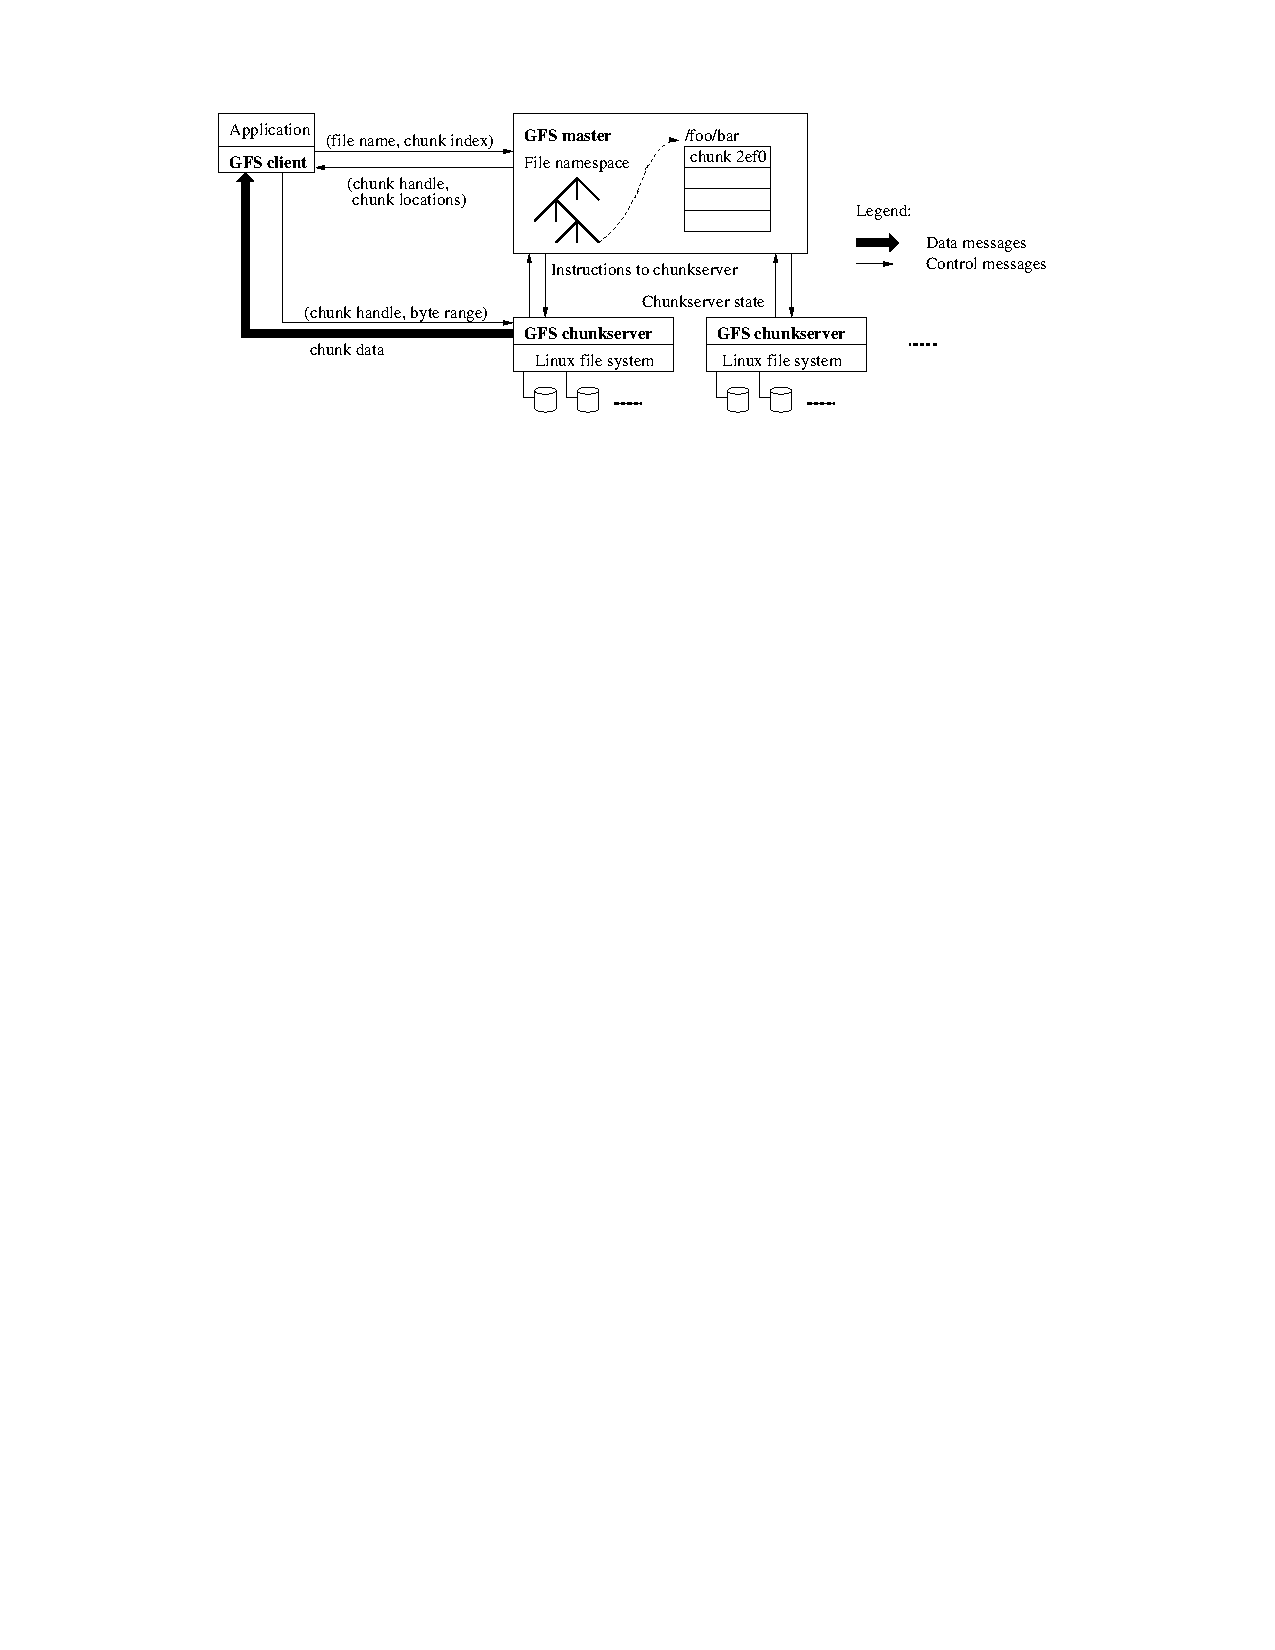
\includegraphics[width=\linewidth]{figs/GFSArchitecture.pdf}
	\caption{The Architecture of GFS \protect \cite{ghemawat2003google}}
	\label{fig:gfs}
\end{figure}

\noindent Files are divided into fixed size \textit{chunks} stored in \textit{chunkservers}. For fault tolerance, each chunk is replicated across multiple chunkservers and the default replication factor is three.

\noindent The \textit{master} is a metadata server maintaining namespace, access control information, the file-chunk mappings and chunks' current locations. Besides, it is also responsible for system-wide activities including garbage collection, chunk lease management, chunk migration between chunkservers.

\noindent Although this single master server architecture simplifies the design of GFS, especially on complexed tasks like chunk placement and replication decisions using global knowledge, yet the master's involvement in reads and writes needs to be minimized otherwise it will become a bottleneck in the system.

\subsection{The Hadoop Distributed File System}

The \textit{Hadoop Distributed File System} (HDFS) is inspired by the Google File System. Initially, HDFS is built for Hadoop Map-Reduce computational framework. With the development of Hadoop ecosystem including HBase~\cite{apachehbase}, Pig~\cite{apachepig}, Mahout~\cite{apachemahout}, Spark~\cite{apachespark}, etc, HDFS becomes the storage layer for other big data applications. Enabling petabytes of data to be persisted on clusters of commodity hardware at relatively low cost, HDFS aims to stream these large data sets at high bandwidth to user applications. Therefore, like GFS, HDFS is optimized for delivering a high throughput of data at the expense of latency~\cite{white2012hadoop}.

\noindent Similar to GFS, HDFS stores metadata and file data separately. The architecture of a HDFS cluster consists of a single \textit{NameNode}, multiple \textit{DataNodes}, and is accessed by multiple \textit{clients} as shown in Figure~\ref{fig:hdfsv1}.

\begin{figure}[ht]
	\centering
	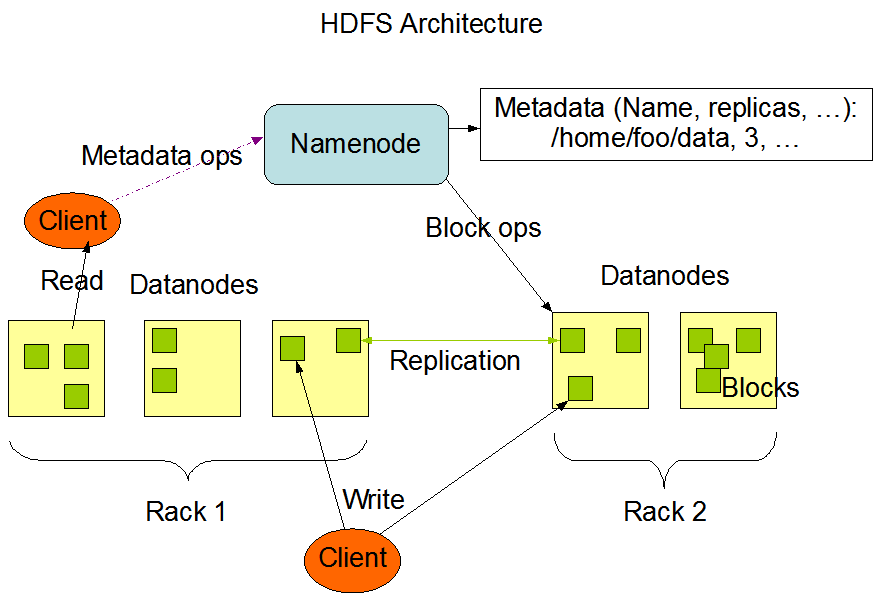
\includegraphics[scale=0.4]{figs/hdfsarchitecturev1.png}
	\caption{The Architecture of HDFS \protect \cite{borthakur2008hdfs}}
	\label{fig:hdfsv1}
\end{figure}

\noindent Files in HDFS are split into smaller blocks stored in \textit{DataNodes}. For fault tolerance, each block is replicated across multiple \textit{DataNodes}.

\noindent The \textit{NameNode} is a single dedicated metadata server maintaining the namespace, access control information, and file blocks mappings to DataNodes. The entire namespace is kept in-memory, called the \textit{image}, of the \textit{NameNode}. Its related persistent record, called the \textit{checkpoint} is stored in the local physical file system. The modification of the \textit{image}, called the \textit{journal}, is also persisted in the local physical file system. Copies of the \textit{checkpoints} and the \textit{journals} can made at other servers for durability. Therefore, the \textit{NameNode} restores the namespace by loading the checkpoint and replaying the journal during its restart.
  %%%%%%%%%%%%%%%%%%%%%%%%%%%%%%%%%%%%%%%%%%%%%%%%%%%%%%%%%%%%%%%%%%%%%%%%%%%%%
  %
%%%%%                      SECOND SECTION
 %%%
  %

\section{Concurrency Control in Transactional Systems}

BBB

  %%%%%%%%%%%%%%%%%%%%%%%%%%%%%%%%%%%%%%%%%%%%%%%%%%%%%%%%%%%%%%%%%%%%%%%%%%%%%
  %
%%%%%                         ANOTHER SECTION
 %%%
  %
\section{Isolation Level in Transactional Systems}

CCC

  %%%%%%%%%%%%%%%%%%%%%%%%%%%%%%%%%%%%%%%%%%%%%%%%%%%%%%%%%%%%%%%%%%%%%%%%%%%%%
  %
%%%%%                          LAST SECTION
 %%%
  %

\section{MySQL Cluster}

DDD

  %
 %%%
%%%%%                            THE END
  %
  %%%%%%%%%%%%%%%%%%%%%%%%%%%%%%%%%%%%%%%%%%%%%%%%%%%%%%%%%%%%%%%%%%%%%%%%%%%%%

%%% Local Variables: 
%%% mode: latex
%%% TeX-master: "tese"
%%% End: 
     

  %%%%%%%%%%%%%%%%%%%%%%%%%%%%%%%%%%%%%%%%%%%%%%%%%%%%%%%%%%%%%%%%%%%%%%%%%%%%%
  %
%%%%%                P A R T   I I  -- Assessment in Hop-HDFS
 %%%
  %

\part{Namespace Concurrency Control and Assessment}
\thispagestyle{empty}
%\vbox to\textheight{
%\vfil
%\chapter*{Ratione Voluptatem}
\thispagestyle{empty}

\newpage
\thispagestyle{empty}

  %%%%%%%%%%%%%%%%%%%%%%%%%%%%%%%%%%%%%%% -*- coding: utf-8; mode: latex -*- %%
  %
%%%%%                         CHAPTER
 %%%
  %

% $Id: 2200-irure-dolor.tex,v 1.1 2007/11/23 09:52:42 david Exp $
% $Log: 2200-irure-dolor.tex,v $
% Revision 1.1  2007/11/23 09:52:42  david
% *** empty log message ***
%
%

  %%%%%%%%%%%%%%%%%%%%%%%%%%%%%%%%%%%%%%%%%%%%%%%%%%%%%%%%%%%%%%%%%%%%%%%%%%%%%
  %
%%%%%                     HEAD MATTER
 %%%
  %

\chapter{Namespace Concurrency Control}
%\addcontentsline{lof}{chapter}{\thechapter\quad Irure Dolor}
%\addcontentsline{lot}{chapter}{\thechapter\quad Irure Dolor}
\label{ch:Locking}

%\begin{quotation}
%  {\small\it Neque porro quisquam est qui dolorem ipsum quia dolor sit amet, consectetur, adipisci velit...}
%
%{\small\it -- Cerico}
%\end{quotation}

\section{Namespace Concurrency Control in GFS}

\subsection{Namespace Structure}
Unlike traditional file systems, GFS doesn't have a per-directory data structure, which means that it doesn't support listing all files in a directory (i.e, \textit{ls} in POSIX), nor aliasing for the same file or directory (i.e, hard or symbolic links). Instead, with prefix compression, GFS represents the namespace as a lookup table mapping full pathnames to metadata logically, which means that the full pathnames are similar to the hash keys in a hash table.

\subsection{Namespace Concurrency Control}
Each node (either an absolute directory name or an absolute file name) in the namespace tree will be associated a \textit{read-write} lock. To prevent deadlock, locks are acquired in a \textit{consistent total order}: first ordered by level, then ordered lexicographically within the same level~\cite{ghemawat2003google}.

\noindent One benefit for the locking scheme in GFS is that it allows concurrent mutations for different files/directories within the same directory. 

\begin{figure}[ht]
	\centering
	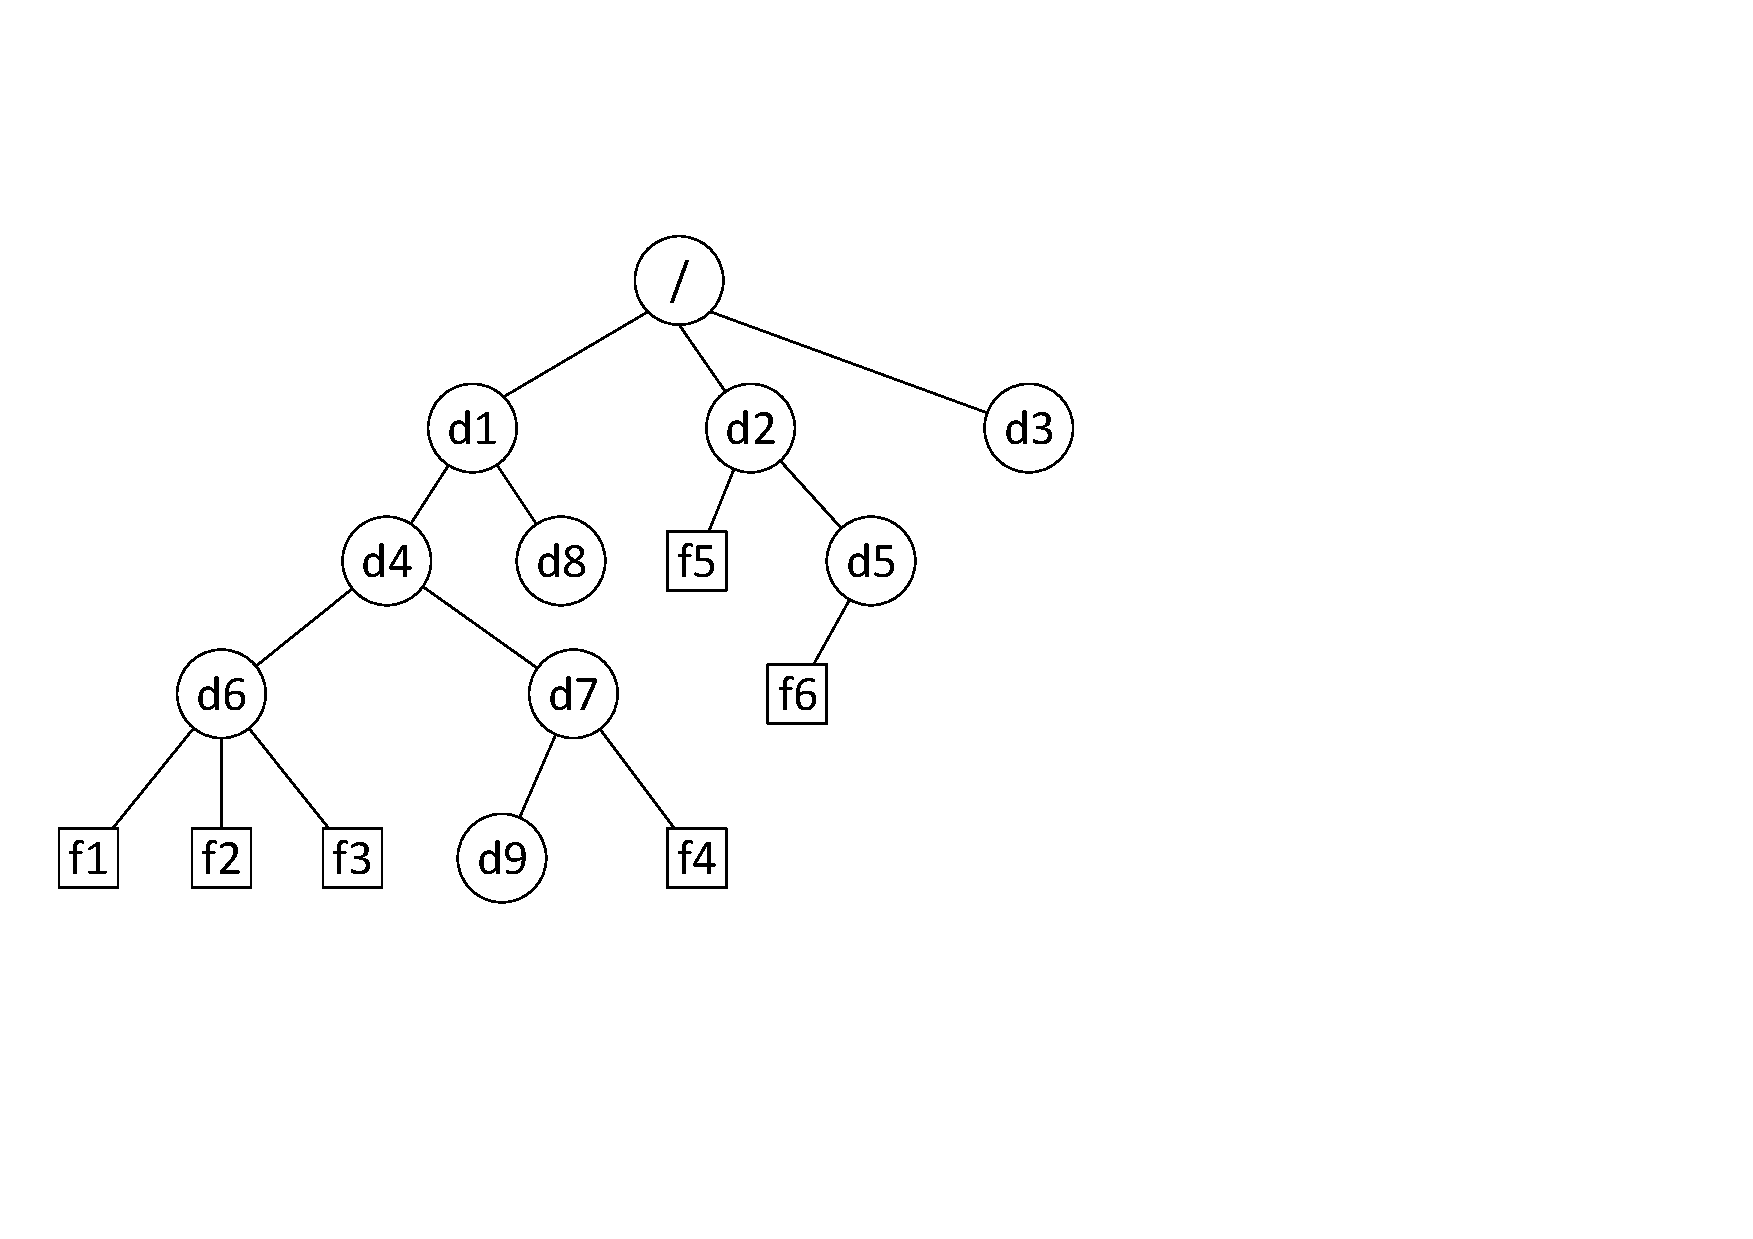
\includegraphics[scale=0.7]{figs/gfstree.pdf}
	\caption{A Graphical Tree Representation for the Namespace in GFS}
	\label{fig:gfsTree}
\end{figure}

\noindent For example, suppose that we have a graphical tree representation for the namespace in GFS as shown in Figure~\ref{fig:gfsTree}. Concurrently, we have five operations involving files \textit{f1, f2, f3, f4} and directory \textit{d9}. As we can see from Table~\ref{table:gfsLock1}, there are no conflicting locks (\textit{Read-Write and Write-Write}), all these five operations are all allowed to happen concurrently.

\begin{table}
	\centering
    \begin{tabular}{|l|c|c|c|c|c|}
    	\hline
    	\textbf{\textit{Total Order Locks}}            & \textbf{Operation1} & \textbf{Operation2} & \textbf{Operation3} & \textbf{Operation4} & \textbf{Operation5} \\ \hline
    	\textbf{\color{red}/ }           & Read1      & Read2      & Read3      & Read4      & Read5      \\ \hline
    	/\textbf{\color{red}d1}          & Read1      & Read2      & Read3      & Read4      & Read5      \\ \hline
    	/d1/\textbf{\color{red}d4}       & Read1      & Read2      & Read3      & Read4      & Read5      \\ \hline
    	/d1/d4/\textbf{\color{red}d6}    & Read1      & Read2      & Read3      & ~          & ~          \\ \hline
    	/d1/d4/\textbf{\color{red}d7}    & ~          & ~          & ~          & Read4      & Read5      \\ \hline
    	/d1/d4/d6/\textbf{\color{red}f1} & Write1     & ~          & ~          & ~          & ~          \\ \hline
    	/d1/d4/d6/\textbf{\color{red}f2} & ~          & Write2     & ~          & ~          & ~          \\ \hline
    	/d1/d4/d6/\textbf{\color{red}f3} & ~          & ~          & Write3     & ~          & ~          \\ \hline
    	/d1/d4/d7/\textbf{\color{red}d9} & ~          & ~          & ~          & Write4     & ~     \\ \hline
    	/d1/d4/d7/\textbf{\color{red}f4} & ~          & ~          & ~          & ~          & Write5          \\ \hline
    \end{tabular}
	\caption{Concurrent Mutations within for different files/directories and Related Read-Write Lock Sets}
	\label{table:gfsLock1}
\end{table}

\noindent Since operations will be serialized properly when trying to obtain conflict locks(\textit{Read-Write and Write-Write}), concurrent mutations on the same file/directory will be prevented.

\begin{table}[ht]
	\centering
	\begin{tabular}{|l|c|c|}
		\hline
		\textbf{\textit{Total Order Locks}}             & \textbf{Operation1} & \textbf{Operation2}                    \\ \hline
		\textbf{\color{red}/}             & Read1      & Read2                         \\ \hline
		/\textbf{\color{red}d1}           & Read1      & Read2                         \\ \hline
		/\textbf{\color{red}d3}           & Read1      & ~                             \\ \hline
		/d1/\textbf{\color{red}d8}        & Write1     & Read2 \textbf{(Conflicts with Write1)} \\ \hline
		/d3/\textbf{\color{red}d8}       & Write1     & ~                             \\ \hline
		/d1/d8/\textbf{\color{red}Qi.txt} & ~          & Write2                        \\ \hline
	\end{tabular}
	\caption{Serialized Concurrent Mutations and Conflict Locks}
	\label{table:gfsLock2}
\end{table}

\noindent For example, if there are another two concurrent operations. \textit{Operation 1} wants to snapshot directory \textit{d8} to be under directory \textit{d3}, but \textit{Operation 2} wants to create a new file \textit{Qi.txt} under directory \textit{d8}. Table~\ref{table:gfsLock2} shows how conflict locks prevent the new file \textit{Qi.txt} being created when directory \textit{d8} is being snapshotting.

\noindent In sum, GFS trades off common file system requirements for this namespace locking scheme with nice concurrency control properties.
  %%%%%%%%%%%%%%%%%%%%%%%%%%%%%%%%%%%%%%%%%%%%%%%%%%%%%%%%%%%%%%%%%%%%%%%%%%%%%
  %
%%%%%                        FIRST SECTION
 %%%
  %

\section{Namespace Concurrency Control in HDFS}

\subsection{Namespace Structure}

Unlike GFS, the interface to HDFS is patterned after UNIX, and it support POSIX like commands (e.g, \textit{ls, mkdir, rm, cp, chown}) to the common file system. The namespace of HDFS is structured as a hierarchy of files and directories. Files and directories are represented on the NameNode by \textit{INodes} with attributes like permissions, modification and access times, namespace and disk space quotas~\cite{borthakur2008hdfs}. Each file is represented by an \textit{INodeFile} object, each directory is represented by an \textit{INodeDirectory}, and each symbolic link is represented by an \textit{INodeSymlink object}. Figure~\ref{fig:inodeuml} shows the Namespace INode Structure in UML diagram with major attributes.

\begin{figure}[h]
	\centering
	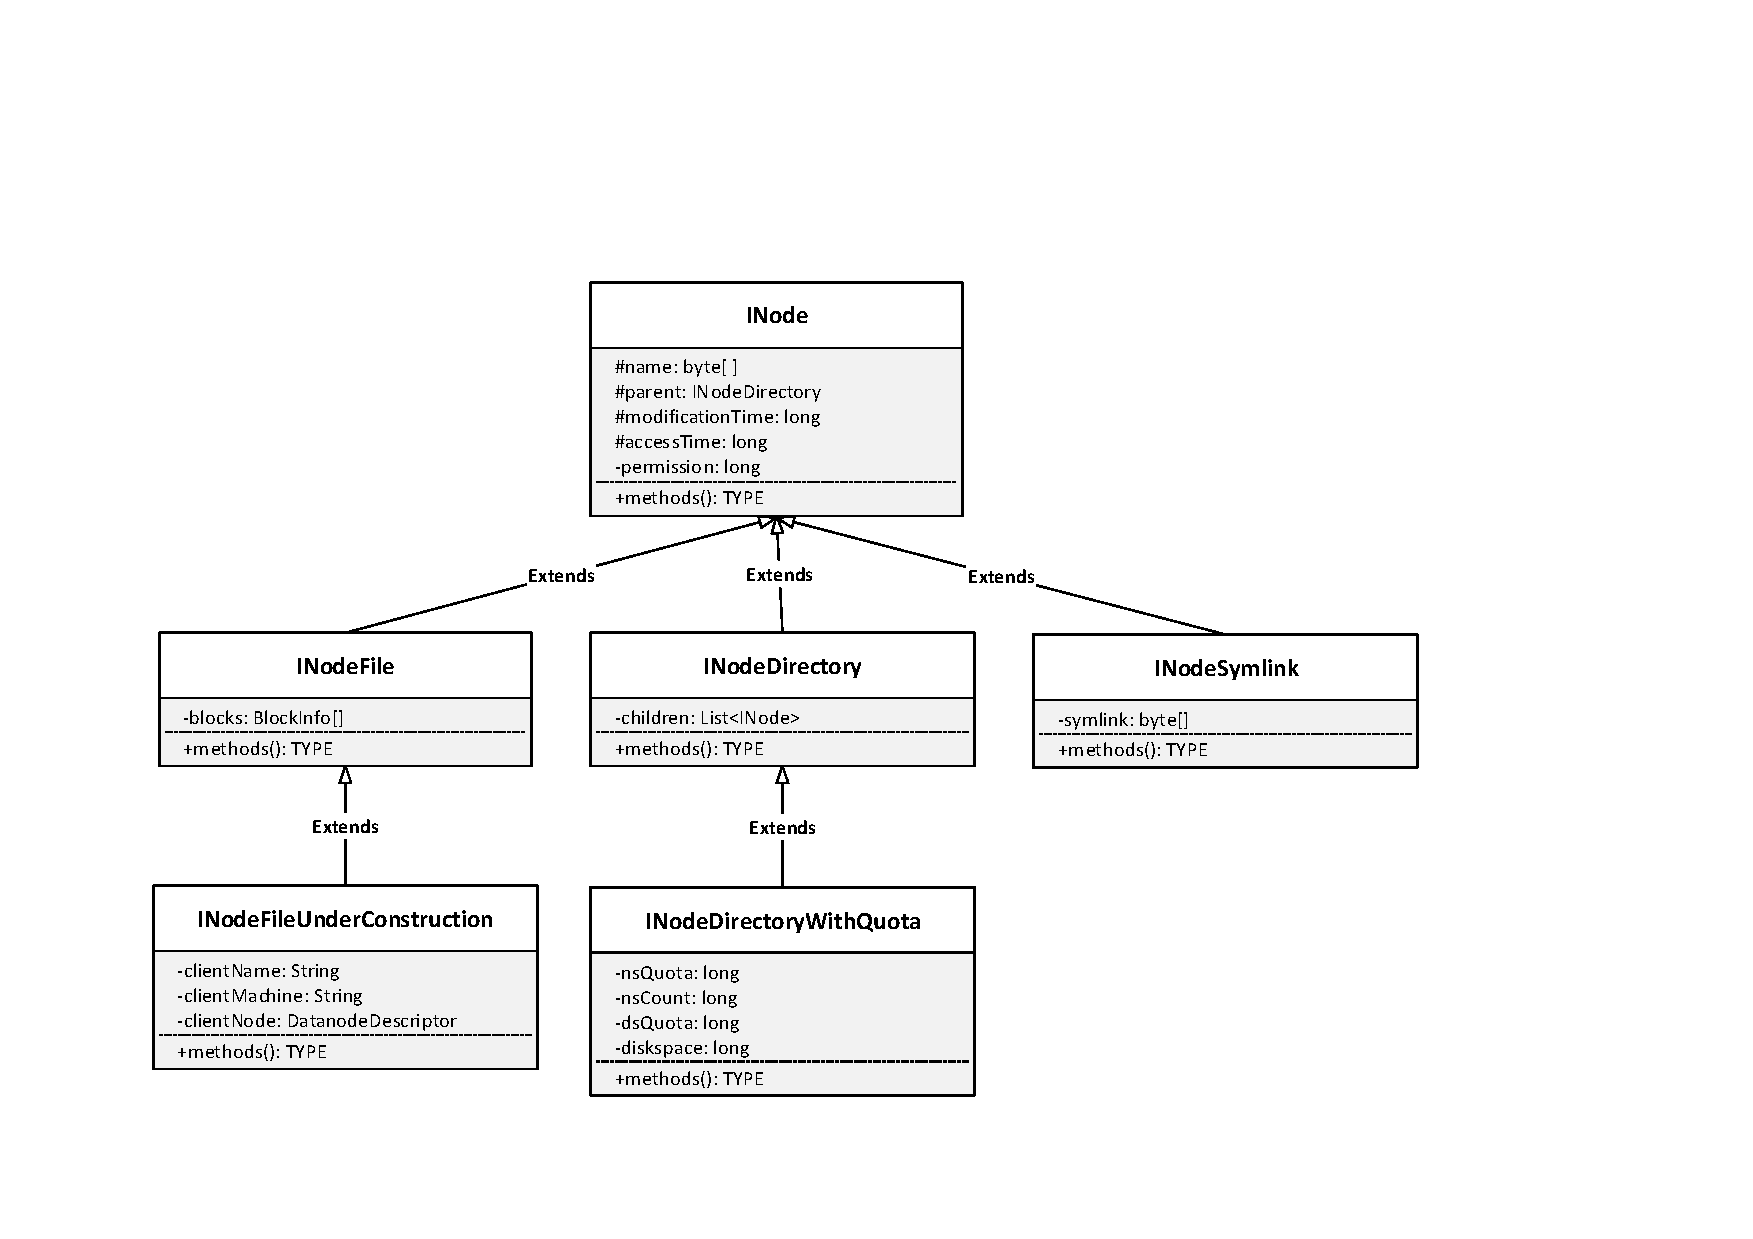
\includegraphics[width=\linewidth]{figs/INodeUML.pdf}
	\caption{The Namespace INode Structure in HDFS}
	\label{fig:inodeuml}
\end{figure}

\subsection{Namespace Concurrency Control}

\noindent The hierarchical INode structure makes HDFS not possible to adopt the namespace locking scheme from GFS. In order to support POSIX like operations (list files, set quotas, create symbolic links), INodeFiles, INodeDirectories and INodeSymlink objects are semantically related to each other, rather than just logical representation.

\noindent For example, suppose that HDFS adopts the namespace locking scheme in GFS. An INodeDirectory \textit{D3} with quota \textit{1} which only allows 1 more INode to be created inside it. Concurrently, there are four operations try to create an INodeFile inside \textit{D3}. All of them put a read lock on \textit{D3} first. Finding that the quota is 1, they then put a write lock on the file and create it under the directory. Finally four files are created under \textit{D3} but it violates the quota. See Figure~\ref{fig:hdfsquota}.

\begin{figure}[h]
	\centering
	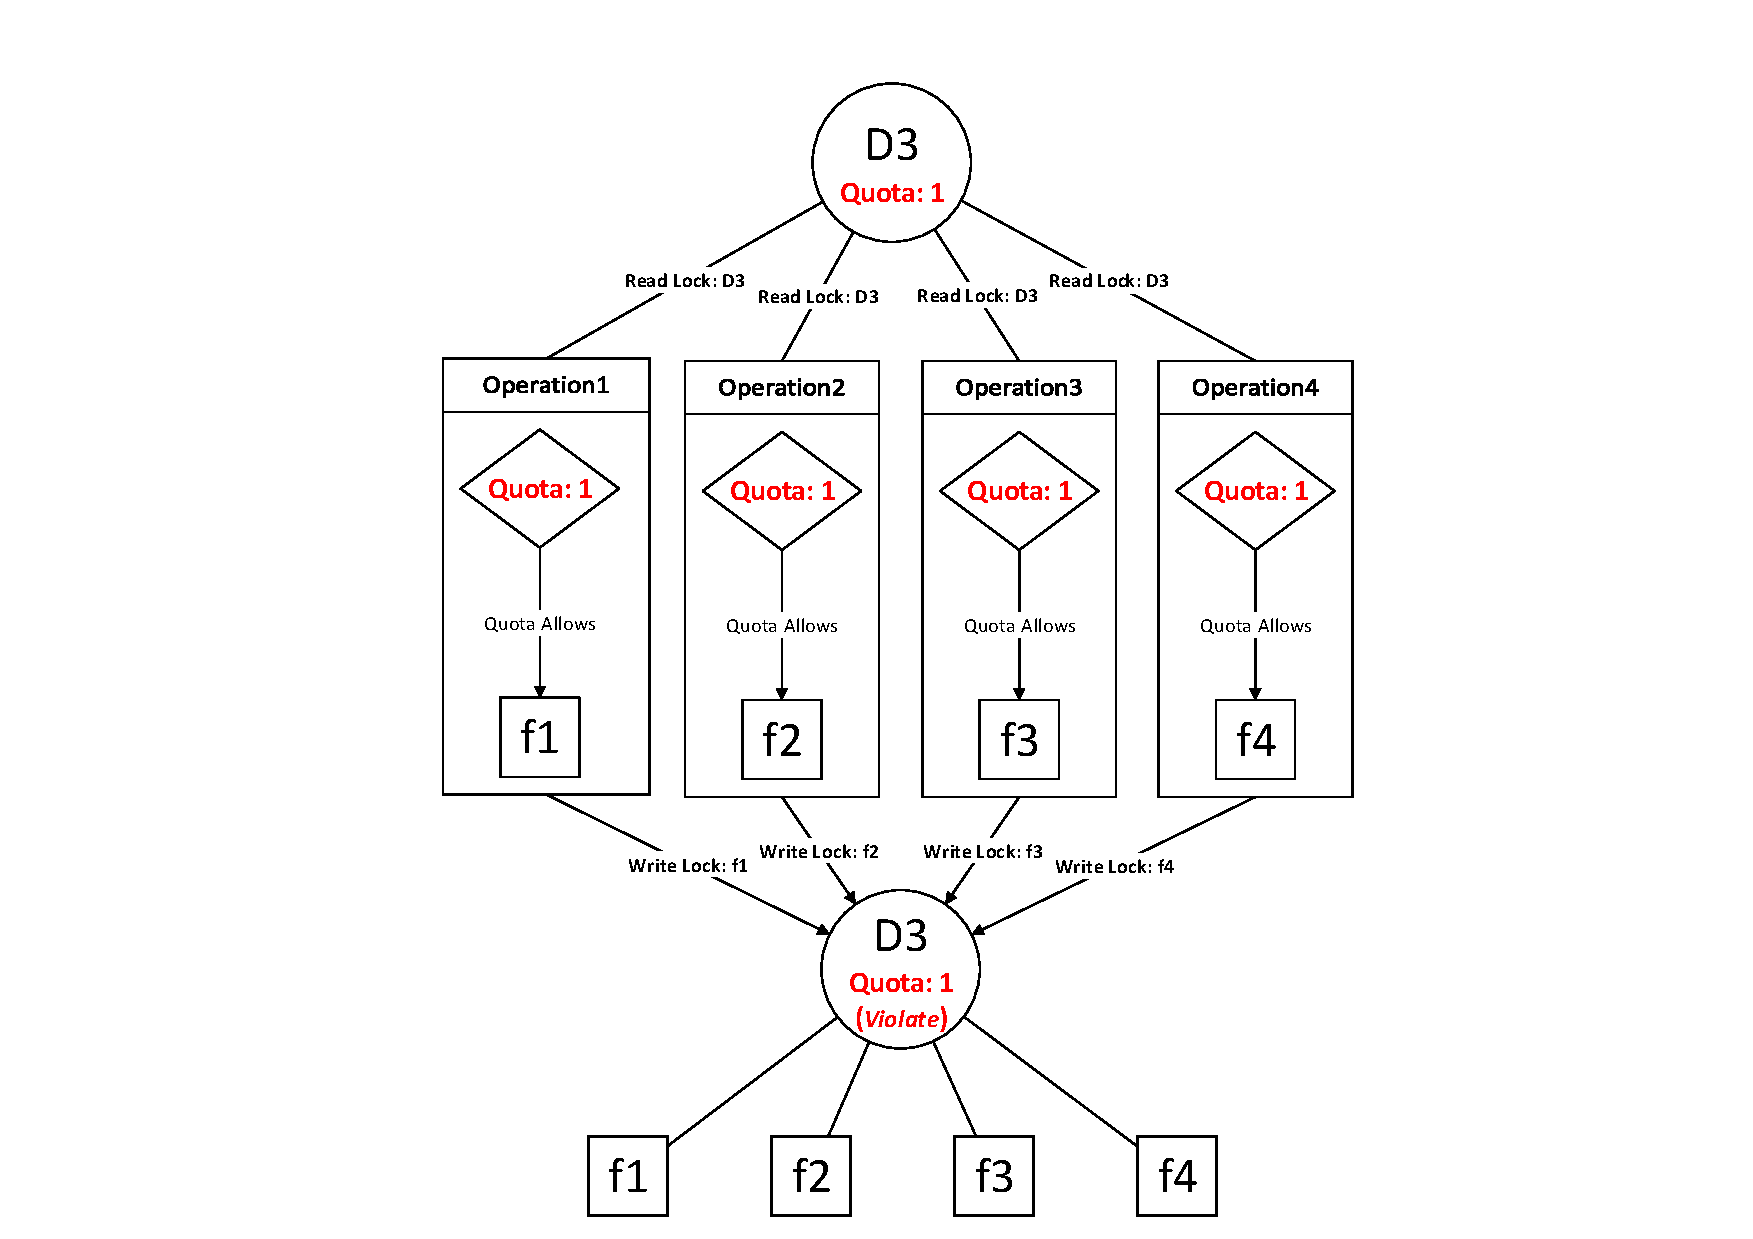
\includegraphics[scale=0.7]{figs/hdfsquota.pdf}
	\caption{Violation in Quota Semantic}
	\label{fig:hdfsquota}
\end{figure}

\noindent One way to solve this consistency problem is to synchronize all the related attributes among different threads under proper semantic group. However, it complicates the namespace design and is not realistic. Therefore, to protect the namespace among parallel running threads, a global read/write lock (fsLock in \textit{FSNamesystem} - \textit{ReentrantReadWriteLock} in java language) is used to maintain the atomicity of the namespace. We call it \textit{system-level lock}.

\noindent HDFS categorizes the metadata operations into \textit{read operations} and \textit{write operations}. Concurrent threads to access the namespace for read operations are allowed, but it restricts a single thread to namespace for write operations. Therefore, all concurrent readers get the same view of the mutated data reflected by completed writes. We call it \textit{Strong Consistency Semantics} in HDFS. (But it is still weaker than the standard POSIX consistency model since it trades some POSIX requirements for performance in terms of data coherency~\cite{white2012hadoop})

\subsection{Limitations}

\noindent Although the namespace is kept in-memory for fast operations, the system-level lock is still the bottleneck in NameNode under high workload pressure. Here we analyze the Remote Procedure Call (RPC) for namespace operations between clients and NameNode. See Figure~\ref{fig:nnRPC} for the process:

\begin{enumerate}[noitemsep]
	\item Client makes an RPC request to NameNode RPC server, like \textit{mkdir}.
	\item The listener thread in NameNode RPC server accepts this request.
	\item The Reader, child thread of Listener, processes the request and makes it as a Call object stored in the Call Queue, waiting for the handling.
	\item One of the handlers gets a Call object (\textit{mkdir}) from the queue. As \textit{mkdir} belongs to write operation, the handler takes a write lock on the namespace.
	\item After taking the write lock, a new directory will be created in the namespace within NameNode.
	\item The modification record needs to be synchronized to the editlogs.
	\item Release the write lock.
	\item The callback is returned to the Responder thread.
	\item The client get the result for this operation (either success or fail).
\end{enumerate}

\noindent As we can see, any of the steps above may become the bottle. But in step 6, while the entire namespace is protected by the system-level lock, the modification record needs to be saved into the editlogs. Since the editlogs are written into the physical hard drives sequentially, the more syn edit to be handled, the slower it will be for the responder to return the callback. The system-level lock won't be released during this process, so the throughput will be decreased greatly during heavy workload.

\begin{figure}[h]
	\centering
	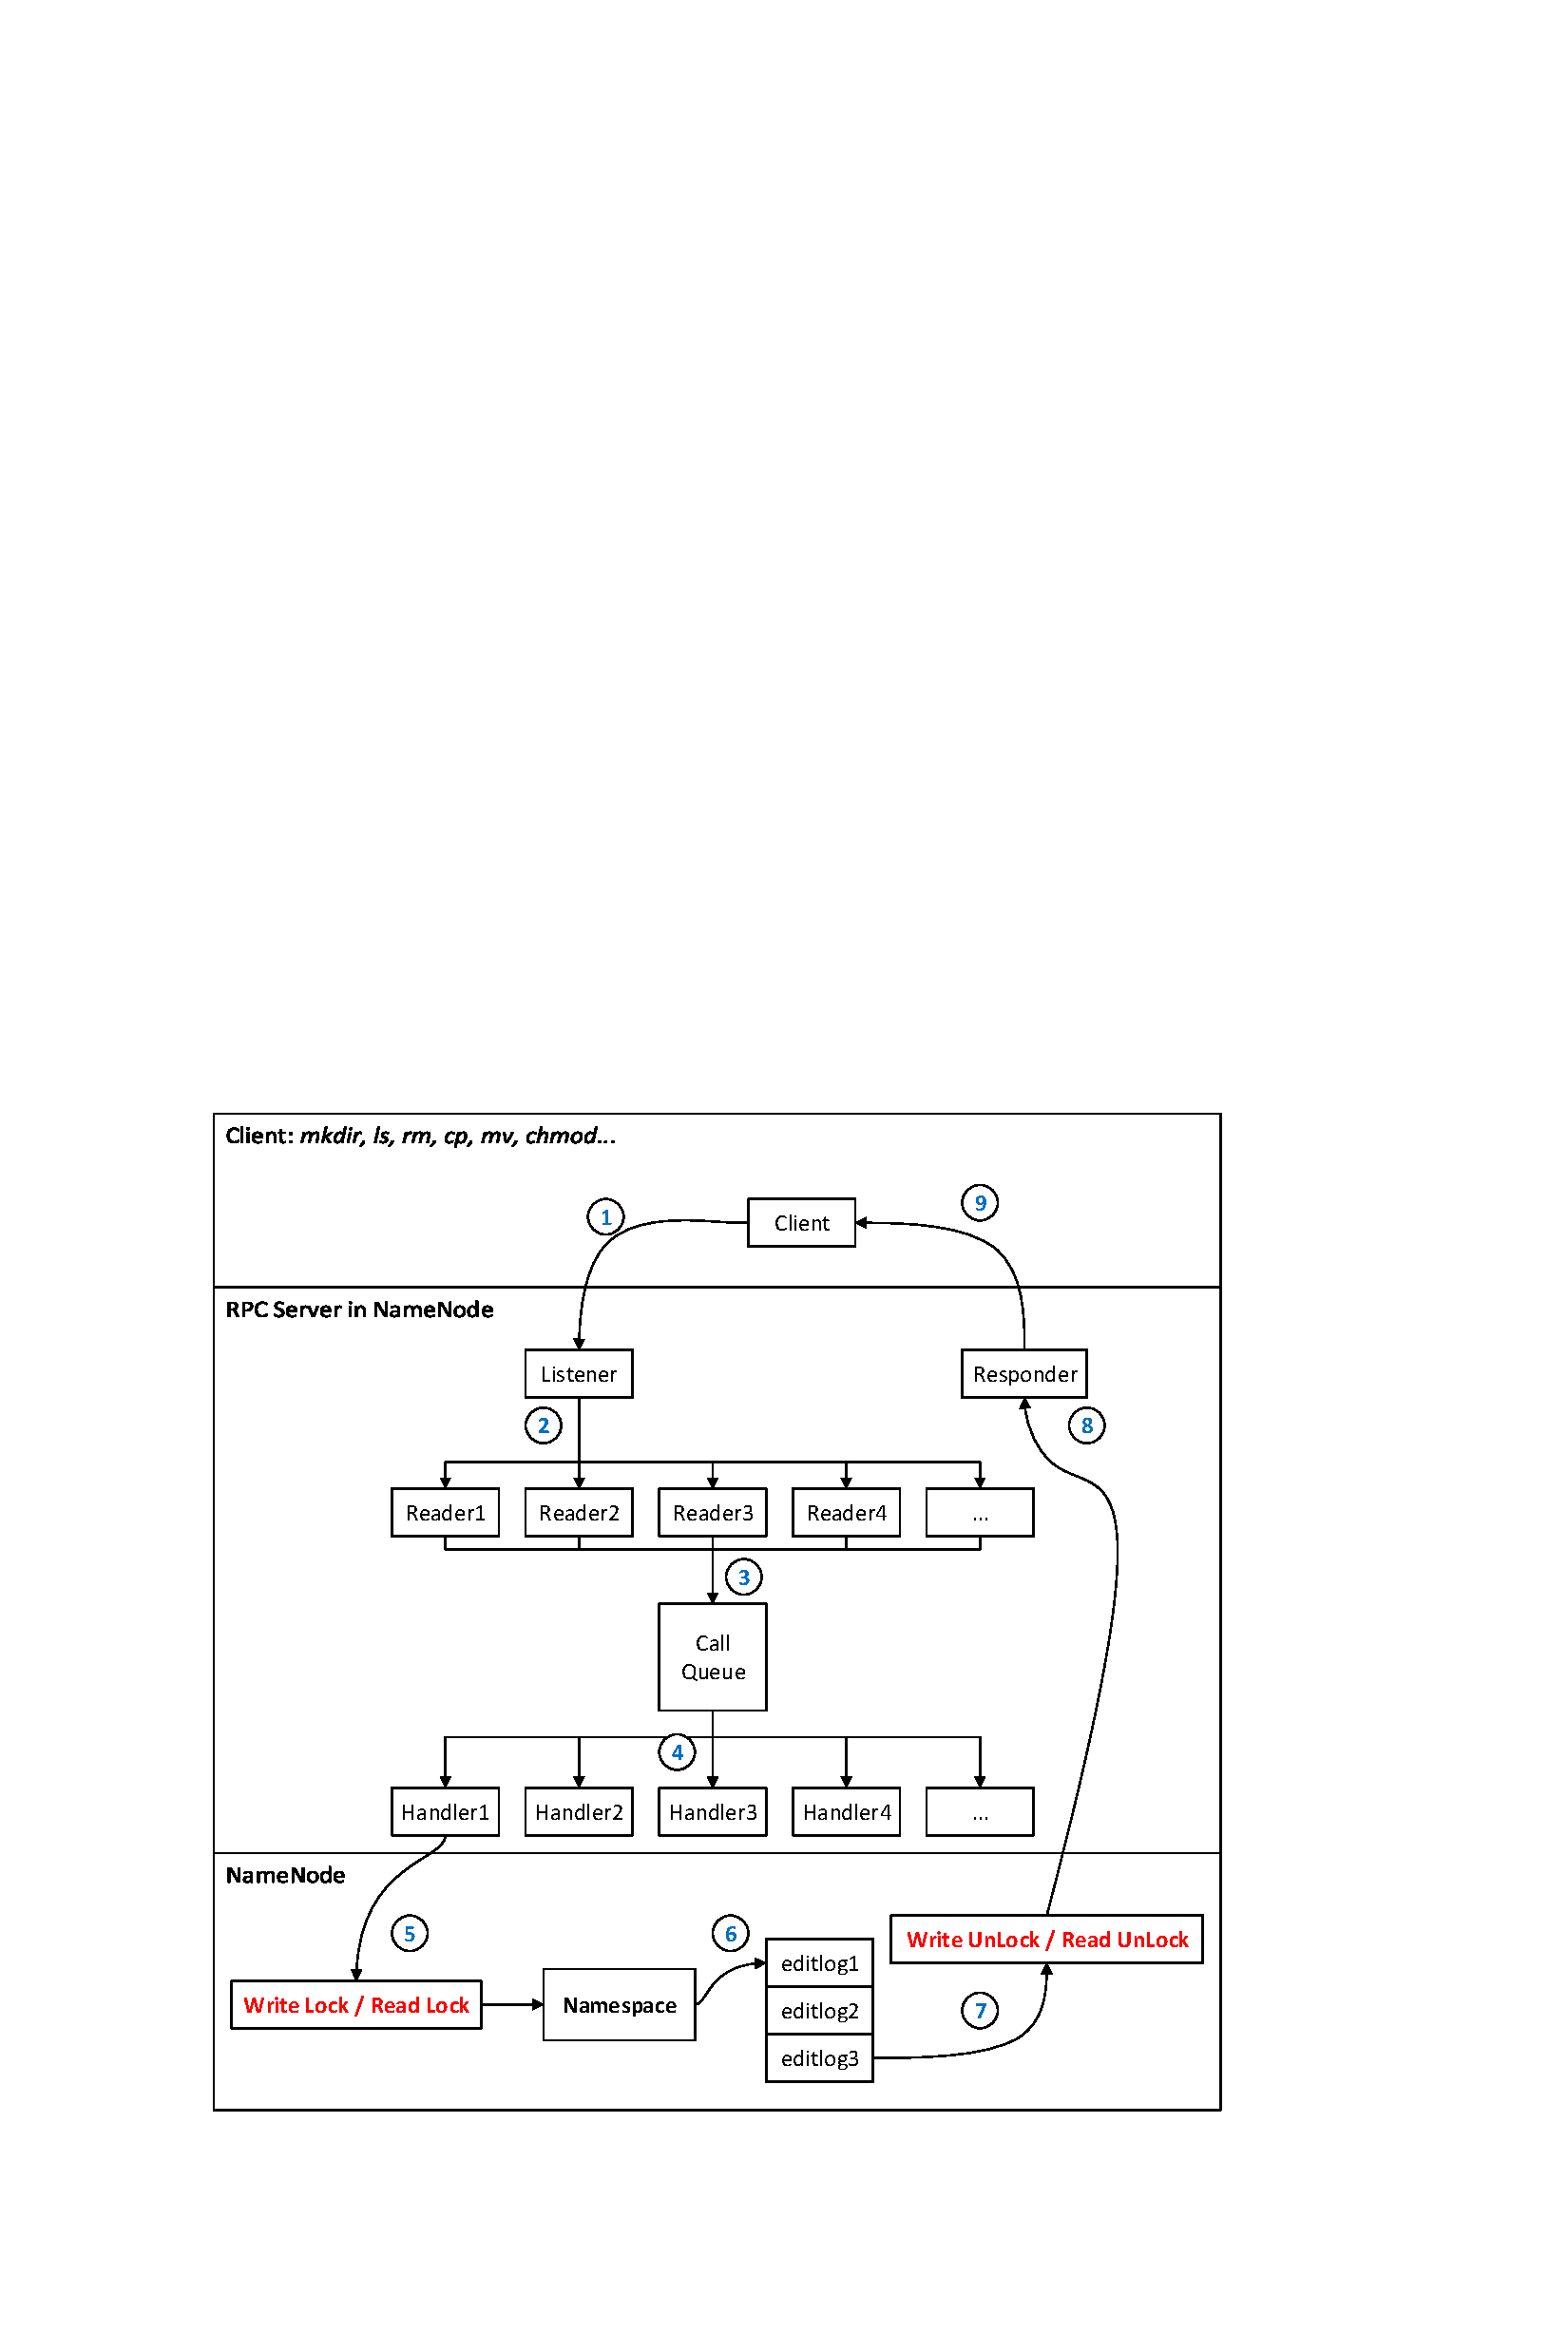
\includegraphics[scale=0.8]{figs/nnRPC.pdf}
	\caption{RPC between Clients and NameNode for Namespace Operations}
	\label{fig:nnRPC}
\end{figure}

  %%%%%%%%%%%%%%%%%%%%%%%%%%%%%%%%%%%%%%%%%%%%%%%%%%%%%%%%%%%%%%%%%%%%%%%%%%%%%
  %
%%%%%                      SECOND SECTION
 %%%
  %

\section{Namespace Concurrency Control in Hop-HDFS}

\subsection{Namespace Structure}
In HDFS, the namespace is kept in-memory as arrays and optimized data structure (like LinkedList) of objects with references for semantic constraints. Therefore, it has a \textit{directed tree structure}, similar to Figure~\ref{fig:gfsTree}. 

\noindent In Hop-HDFS, the namespace is stored into tables of MySQL Cluster database, so all INode objects are represented as individual row records in a single \textit{inodes table}. In order to preserve the directed tree structure, we add an id column and a parent\_id column to each row of in \textit{inodes table}. Therefore, the graphical representation of the filesystem hierarchy for INodes is like Figure~\ref{fig:hoptree}. The table representation in the database is like Table~\ref{table:hoptreeTable}.

\begin{figure}[h]
	\centering
	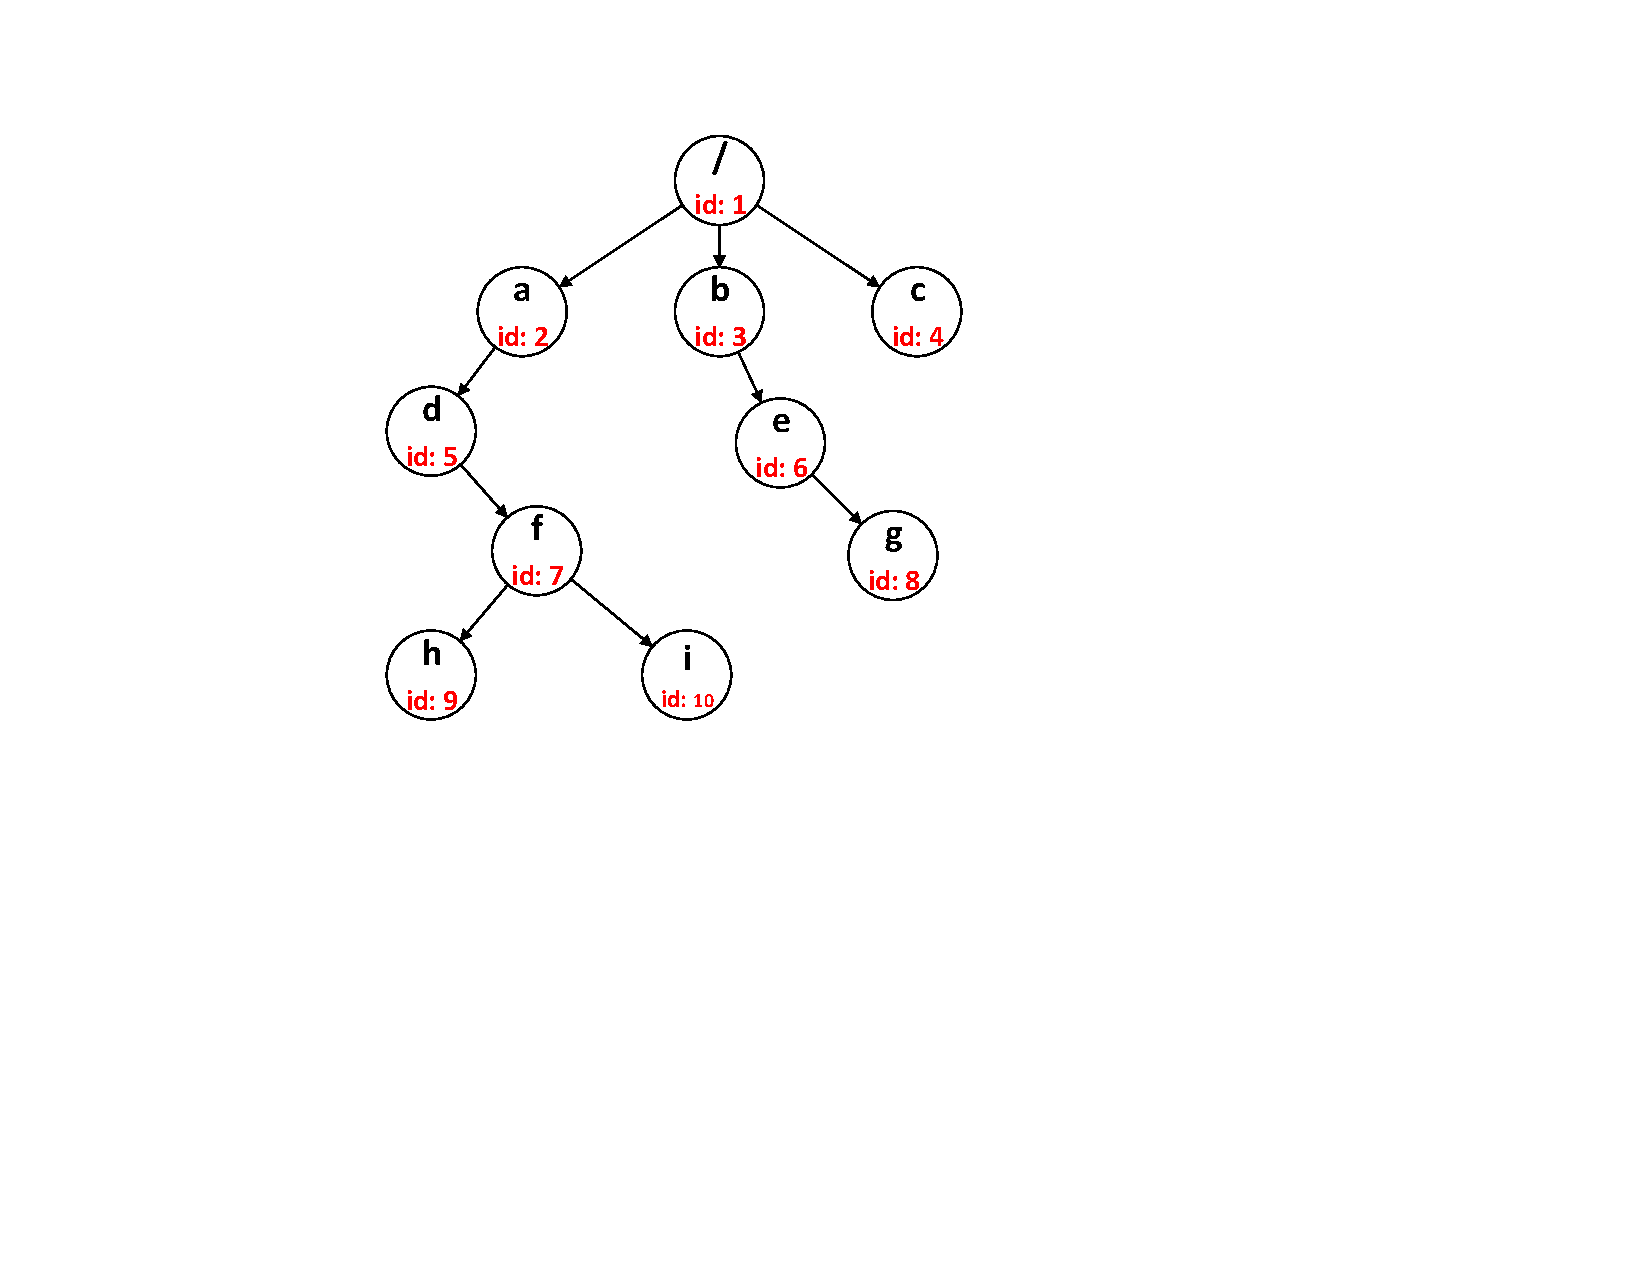
\includegraphics[scale=1]{figs/hoptree.pdf}
	\caption{Filesystem Hierarchy with ID for INodes in Hop-HDFS}
	\label{fig:hoptree}
\end{figure}

\begin{table}[h]
	\centering
	\begin{tabular}{|c|c|c|c|}
		\hline
		\textbf{id} & \textbf{parent\_id} & \textbf{name} & \textbf{other parameters...} \\ \hline
		1 & 0 & / & ... \\ \hline
		2 & 1 & a & ... \\ \hline
		3 & 1 & b & ... \\ \hline
		4 & 1 & c & ... \\ \hline
		5 & 2 & d & ... \\ \hline
		6 & 3 & e & ... \\ \hline
		7 & 5 & f & ... \\ \hline
		8 & 6 & g & ... \\ \hline
		9 & 7 & h & ... \\ \hline
		10 & 7 & i & ... \\ \hline
	\end{tabular}
	\caption{INode Table for Hop-HDFS}
	\label{table:hoptreeTable}
\end{table}

\noindent Since the \textit{id} is unique and atomically generated for INodes in each new transaction, the \textit{Primary Key} for the table is $<$name, parent\_id$>$ pair to avoid duplicated data rows during primary key lookup. Besides, the INode \textit{id} is not known beforehand on the application side, but the $<$name, parent\_id$>$ pair is known since it is stored as a path string. So data rows can be looked up by the $<$name, parent\_id$>$ pair \textit{Primary Key} directly from database.

\noindent With the \textit{id} and \textit{parent\_id} relationship, the hierarchy will be constructed correctly from the rows to be in-memory objects used by the name system.

\subsection{Namespace Concurrency Control}

In the first version of Hop-HDFS~\cite{wasif2012distributed} (also named as KTHFS), the main task is to migrate the metadata from memory to MySQL Cluster. Therefore, it still depends on the system-level lock in HDFS NameNode (fsLock in \textit{FSNamesystem} - \textit{ReentrantReadWriteLock} to serialize the operations and maintain the semantics. This becomes a big problem since the network latency between NameNode and database is far more larger than it was when operated inside memory in original HDFS. Each operation takes a long time lock on the filesystem. The throughput heavily decreases. A fine grained locking scheme is needed to improve the concurrency.

\noindent In the second version of Hop-HDFS~\cite{peiro2013maintaining} (also named as KTHFS), it adopts a fine-grained row-level locking mechanism to improve the throughput while maintaining the strong consistency semantics. It uses transactions with \textit{Pessimistic Concurrency Control} (PCC) to ensure the safety and progress of metadata operations. 

\noindent Based on a hierarchical concurrency model, it builds a \textit{directed acyclic graph} (DAG) for the namespace. Metadata operation that mutates the DAG either commit or abort (for partial failures) in a single transaction. See Figure~\ref{fig:dag}.

\begin{figure}[h]
	\centering
	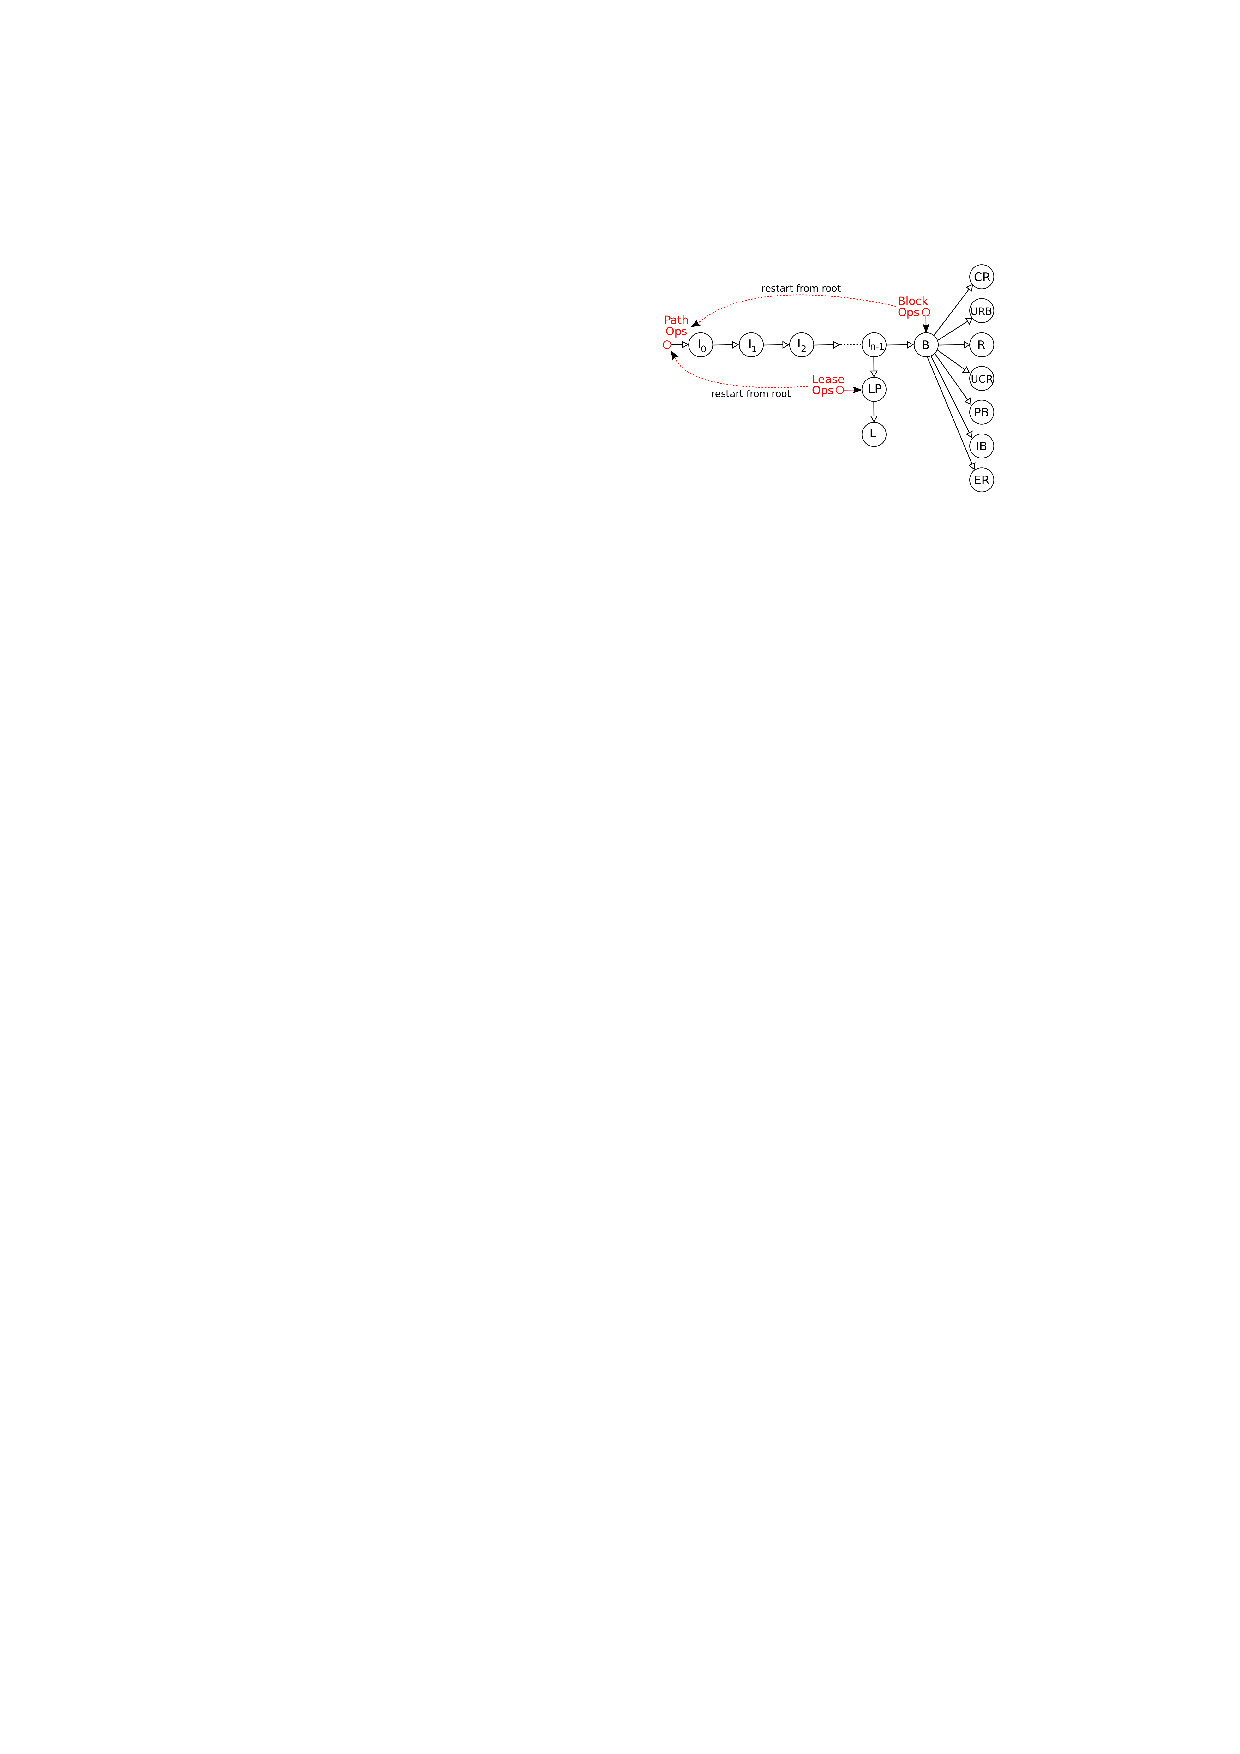
\includegraphics[scale=2]{figs/dag.pdf}
	\caption{Acyclic DAG. Operations start from root, locks taken in order from leftmost child \protect \cite{hakimzadeh2014scaling} 
		\\ \textit{I: INode, B: BlockInfo, L: Lease, LP: LeasePath, CR: CorruptedReplica, URB: UnderReplicatedBlock, R: Replica, UCR: UnderConstructionReplica, PB: PendingBlock, IB: InvalidBlock, ER: ExcessReplica}}
	\label{fig:dag}
\end{figure}

\noindent Besides, \textit{implicit locking}~\cite{gray1976granularity} is used to lock on the data row of the root of a subtree in a transaction, which implicitly acquires locks on all the descendants, so that the strong consistent semantics in original HDFS can be maintained.

\subsection{Limitations}

\noindent There are two major limitations in this locking scheme:
\begin{enumerate}[noitemsep]
	\item It lowers the concurrency when multiple transactions try to mutate different descendants within the same subtree. Only one writer is allowed to work on INodes under one directory due to the implicit lock (Write Lock) for parent directory.
	
	 For example, if transaction Tx1 wants to mutate INode \textit{h}, and another transaction Tx2 wants to mutate INode \textit{i} concurrently in Figure~\ref{fig:hoptree}. Tx1 will take a parent lock on INode \textit{f} first and then perform operations. No more transactions can work under INode \textit{f} anymore. Tx2 will be blocked by the implicit lock until Tx1 commits. See Table~\ref{table:hoplockTable}.
	
	\item There is un-avoided duplicated database round trips overhead. It takes two transactions to finish the implicit locking. The first transaction is used to resolve the path in the database so that we know which rows existed in the database so that the INode's parent directory can be taken the implicit write lock in the second transaction, or last existing INode directory can be taken the implicit write lock if the path is not full resolved(HDFS will build up the missing intermediate INodeDirectories).
	
	 For example, if transaction Tx1 wants to mutate INode \textit{h} in Figure~\ref{fig:hoptree}, in the first database round trip, it needs to resolve the path to see if the related rows of INode\textit{ /, a, d, f, h} are all in the database. If yes, in the second database round trip, INode\textit{ /, a, d} will be taken Read Locks~\footnote{The third version of Hop-HDFS is trying to Replace Read Lock to Read\_Committed for this PCC scheme} and the INode \textit{f} will be taken a Write Lock; if no, the last existing INode will be taken a Write Lock while others will be taken Read Locks.
\end{enumerate}

\begin{table}[h]
	\centering
	\begin{tabular}{|c|c|c|c|c|}
		\hline
		\textbf{id} & \textbf{parent\_id} & \textbf{name} & \textbf{Locks by Tx1} & \textbf{Locks by Tx2} \\ \hline
		1 & 0 & / & Read Lock & Read Lock \\ \hline
		2 & 1 & a & Read Lock & Read Lock \\ \hline
		3 & 1 & b & ~ & ~ \\ \hline
		4 & 1 & c & ~ & ~ \\ \hline
		5 & 2 & d & Read Lock & Read Lock\\ \hline
		6 & 3 & e & ~ & ~ \\ \hline
		7 & 5 & f  & Write Lock & Write Lock \\ \hline
		8 & 6 & g & ~ & ~ \\ \hline
		9 & 7 & h (Mutated by Tx1) & Write Lock (Implicit) & Write Lock (Implicit)\\ \hline
		10 & 7 & i (Mutated by Tx2) & Write Lock (Implicit) & Write Lock (Implicit)\\ \hline
	\end{tabular}
	\caption{Implicit Lock Table in Hop-HDFS}
	\label{table:hoplockTable}
\end{table}
  %%%%%%%%%%%%%%%%%%%%%%%%%%%%%%%%%%%%%%% -*- coding: utf-8; mode: latex -*- %%
  %
%%%%%                         CHAPTER
 %%%
  %

% $Id: 2300-omnis-iste-natus.tex,v 1.2 2007/11/23 10:14:54 david Exp $
% $Log: 2300-omnis-iste-natus.tex,v $
% Revision 1.2  2007/11/23 10:14:54  david
% Bug fixes galore.
%
% Revision 1.1  2007/11/23 09:52:42  david
% *** empty log message ***
%
%

  %%%%%%%%%%%%%%%%%%%%%%%%%%%%%%%%%%%%%%%%%%%%%%%%%%%%%%%%%%%%%%%%%%%%%%%%%%%%%
  %
%%%%%                     HEAD MATTER
 %%%
  %

\chapter{Systematic Assessment of Operation Performance in HOP-HDFS}
%\addcontentsline{lof}{chapter}{\thechapter\quad Irure Dolor}
%\addcontentsline{lot}{chapter}{\thechapter\quad Irure Dolor}
\label{ch:Assessment}

\begin{quotation}
  {\small\it Neque porro quisquam est qui dolorem ipsum quia dolor sit amet, consectetur, adipisci velit...}

{\small\it -- Cerico}
\end{quotation}


  %%%%%%%%%%%%%%%%%%%%%%%%%%%%%%%%%%%%%%%%%%%%%%%%%%%%%%%%%%%%%%%%%%%%%%%%%%%%%
  %
%%%%%                        FIRST SECTION
 %%%
  %

\section{A}

AAA

  %%%%%%%%%%%%%%%%%%%%%%%%%%%%%%%%%%%%%%%%%%%%%%%%%%%%%%%%%%%%%%%%%%%%%%%%%%%%%
  %
%%%%%                      SECOND SECTION
 %%%
  %

\section{B}

BBB

\subsection{B1}

BBB1

\subsection{B2}

BBB2

  %%%%%%%%%%%%%%%%%%%%%%%%%%%%%%%%%%%%%%%%%%%%%%%%%%%%%%%%%%%%%%%%%%%%%%%%%%%%%
  %
%%%%%                         ANOTHER SECTION
 %%%
  %
\section{C}

CCC

  %%%%%%%%%%%%%%%%%%%%%%%%%%%%%%%%%%%%%%%%%%%%%%%%%%%%%%%%%%%%%%%%%%%%%%%%%%%%%
  %
%%%%%                          LAST SECTION
 %%%
  %

\section{D}

DDD

  %
 %%%
%%%%%                           THE END
  %
  %%%%%%%%%%%%%%%%%%%%%%%%%%%%%%%%%%%%%%%%%%%%%%%%%%%%%%%%%%%%%%%%%%%%%%%%%%%%%

%%% Local Variables: 
%%% mode: latex
%%% TeX-master: "tese"
%%% End: 


  %%%%%%%%%%%%%%%%%%%%%%%%%%%%%%%%%%%%%%%%%%%%%%%%%%%%%%%%%%%%%%%%%%%%%%%%%%%%%
  %
%%%%%               P A R T   I I I  --  Solution
 %%%
  %

\part{Solution}
\thispagestyle{empty}
%\vbox to\textheight{
%\vfil
%\chapter*{Laborum et Dolorum}
\thispagestyle{empty}

\newpage
\thispagestyle{empty}

  %%%%%%%%%%%%%%%%%%%%%%%%%%%%%%%%%%%%%%% -*- coding: utf-8; mode: latex -*- %%
  %
%%%%%                       CHAPTER
 %%%
  %

% $Id: 3100-nihil-molestiae.tex,v 1.1 2007/11/23 09:52:43 david Exp $
% $Log: 3100-nihil-molestiae.tex,v $
% Revision 1.1  2007/11/23 09:52:43  david
% *** empty log message ***
%
%

  %%%%%%%%%%%%%%%%%%%%%%%%%%%%%%%%%%%%%%%%%%%%%%%%%%%%%%%%%%%%%%%%%%%%%%%%%%%%%
  %
%%%%%                    HEAD MATTER
 %%%
  %

\chapter{Design and Implementation}
The solution we propose to improve the throughput is based on the following four phases:
\begin{enumerate}[noitemsep]
	\item \textbf{Read Phase}: resolving the semantic related group and cache the snapshot copy within the handling transaction.
	\item \textbf{Execution Phase}: transaction read/write operations are performed on its own snapshot and never fetch data from database.
	\item \textbf{Validation Phase}: snapshot's related data rows are fetched from the database. If all their versions match with the original copy of the snapshot, go to update phase; else, abort and retry current transaction.
	\item \textbf{Update Phase}: update related data in the database table. Abort and retry transaction if the instance already exists in the database for "new" data. Increase the versions of the modified rows by 1 if updated successfully.
\end{enumerate}
\label{ch:Design}

\noindent The phases mentioned above will be illustrated detailedly in the following sections.
\section{Resolving the Semantic Related Group}

Resolving the semantic related group for each transaction is the fundamental step to preclude \textit{anomalies} in our implementation. The \textit{constraint violation}~\cite{berenson1995critique} between individual data is formed within a semantic related group. In Hop-HDFS, each metadata operation is implemented as an individual transaction running by a worker thread. Any metadata operation related to the namespace will have one or two input parameters, called \textit{Path}. Here's two examples for methods in the Filesystem API:

\begin{itemize}[noitemsep]
	\item boolean \textbf{mkdirs} (Path \textit{f}): \textit{f} is the path of the INodeDirectory to be created
	\item boolean \textbf{rename} (Path \textit{src}, Path \textit{dst}): \textit{src} is the path to be renamed, \textit{dst} is the new path after rename
\end{itemize} 

\noindent Each \textit{Path} object is related to a string representation of the "/" based absolute path name. For example, in Figure~\ref{fig:hoptree}, the path for INode \textit{h} is: 
\begin{center}
	/a/d/f/h
\end{center}

\noindent Therefore, with the preservation of the \textit{directed tree structure}, we can resolving a semantic related group for each INode along the edge of ancestors as a \textit{LinkedList}. The semantic related group representation for INode \textit{h} is:
\begin{center}
	h: \{/-$>$a-$>$d-$>$f\}
\end{center}

\noindent In other words, when mutating INode \textit{h}, all the semantic constraint can be found within INodes \textit{/, a, d, f}. With this knowledge, we can maintain the strong consistency semantics of original HDFS.

\noindent For each row in \textit{inodes table}, the $<$name, parent\_id$>$ pair is the \textit{Primary Key}. We can get its semantic related rows by primary key lookups directly from database as shown in Table~\ref{table:semanticrelatedTable}. No transactions needed during the \textit{Read Phase} for resolving the semantic related group.

\begin{table}[h]
	\centering
	\begin{tabular}{|c|c|c|c|c|}
		\hline
		~ & \textbf{id} & \textbf{parent\_id} & \textbf{name} & \textbf{other parameters...} \\ \hline
		Related * & 1 & 0 & / & ... \\ \hline
		Related * & 2 & 1 & a & ... \\ \hline
		~ & 3 & 1 & b & ... \\ \hline
		~ & 4 & 1 & c & ... \\ \hline
		Related * & 5 & 2 & d & ... \\ \hline
		~ & 6 & 3 & e & ... \\ \hline
		Related * & 7 & 5 & f & ... \\ \hline
		~ & 8 & 6 & g & ... \\ \hline
		Selected \checkmark & 9 & 7 & h & ... \\ \hline
		~ & 10 & 7 & i & ... \\ \hline
	\end{tabular}
	\caption{Table Representation for the Semantic Related Group}
	\label{table:semanticrelatedTable}
\end{table}
  %%%%%%%%%%%%%%%%%%%%%%%%%%%%%%%%%%%%%%%%%%%%%%%%%%%%%%%%%%%%%%%%%%%%%%%%%%%%%
  %
%%%%%                      SECOND SECTION
 %%%
  %

\section{Per-Transaction Snapshot Isolation}

As we mentioned before, MySQL Cluster supports only the READ COMMITTED transaction isolation level, which means that the committed results of write operations in transactions will be exposed by reads in other transactions. Within a long running transaction, it could read two different versions of data, known as \textit{fuzzy read}, and it could also get two different sets of results if the same query is issued twice, known as \textit{phantom read}.

\noindent \textit{Snapshot isolation} guarantees that all reads made within a transaction see a consistent view of at the database. At the beginning of the transaction, it reads data from a snapshot of the latest committed value. During transaction execution, reads and writes are performed on the this snapshot.

\noindent In commercial database management systems, like Microsoft SQL Server, Oracle, etc, \textit{snapshot isolation} is implemented within multi version concurrency control (MVCC)~\cite{berenson1995critique} on database server side. However, we need to implement snapshot isolation on the application side since MySQL Cluster supports only the READ COMMITTED isolation level.

\noindent After resolving the semantic related group, we take a snapshot on selected rows as well as all related rows of the committed values from database. This snapshot will be cached in-memory within its transaction. Each transaction will have its own copy of snapshot during the lifetime. All transaction operations will be performed on its own snapshot. Therefore, we called it Per-Transaction Snapshot Isolation.

\noindent Before validation phase, the transaction will never fetch any data from database since it has all the semantic related rows in the cache. Therefore, the snapshot provides a consistent view of data for each transaction from read phase until validation phase: 
\begin{itemize}[noitemsep]
	\item \textit{Fuzzy Read} is precluded by \textit{snapshot isolation}: As we can see from Figure~\ref{fig:snapfuzzy}, the second read of Transaction 1 read from snapshot instead of database, not affected by the value committed by Transaction 2.
	
	\begin{figure}[h]
		\centering
		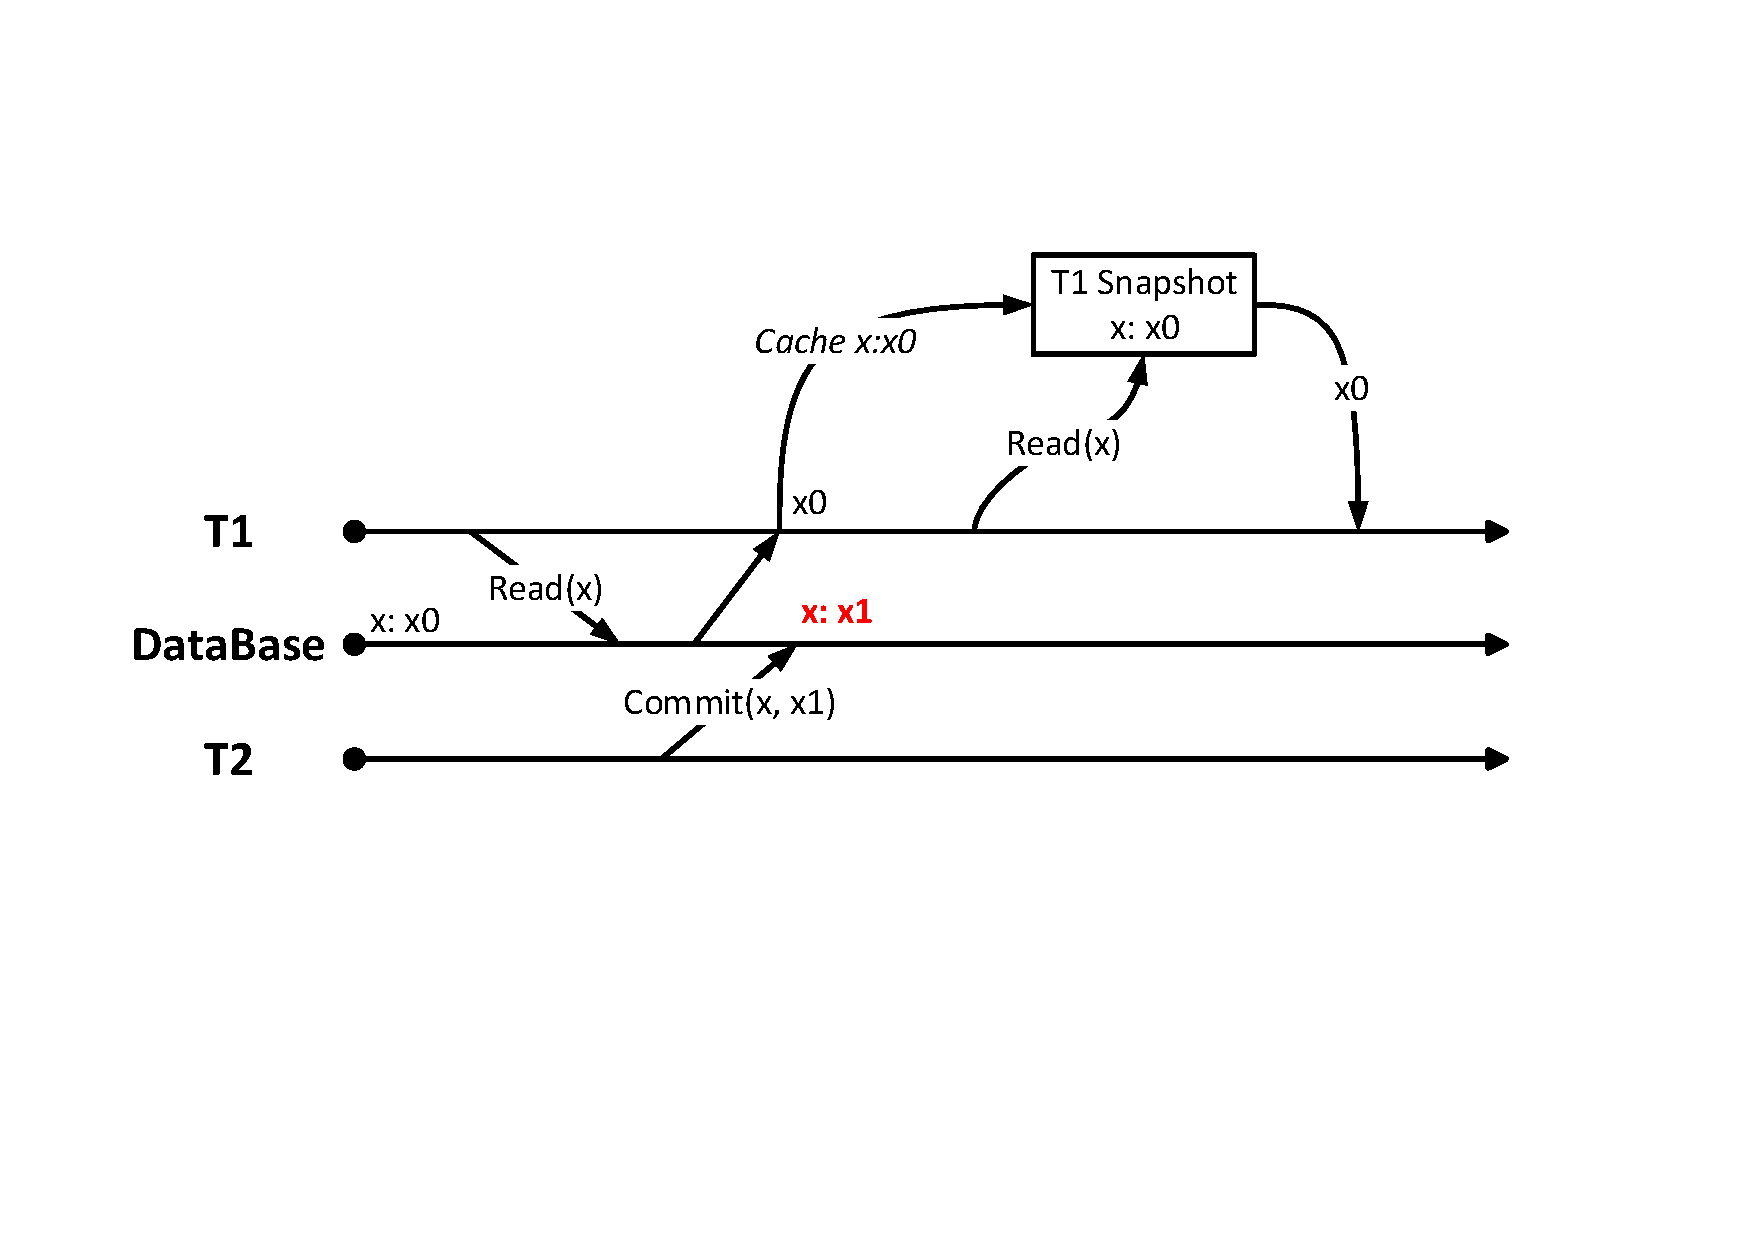
\includegraphics[width=\linewidth]{figs/snapfuzzy.pdf}
		\caption{Snapshot Isolation Precludes Fuzzy Read}
		\label{fig:snapfuzzy}
	\end{figure}
	
	\item \textit{Phantom Read} is also precluded by \textit{snapshot isolation with Semantic Related Group}: As we can see from Figure~\ref{fig:snapphantom}, Transaction 1 snapshot the semantic related group of x after the first count operation. So its second count operation is not affected by the value inserted by Transaction 2.
	
	\begin{figure}[h]
		\centering
		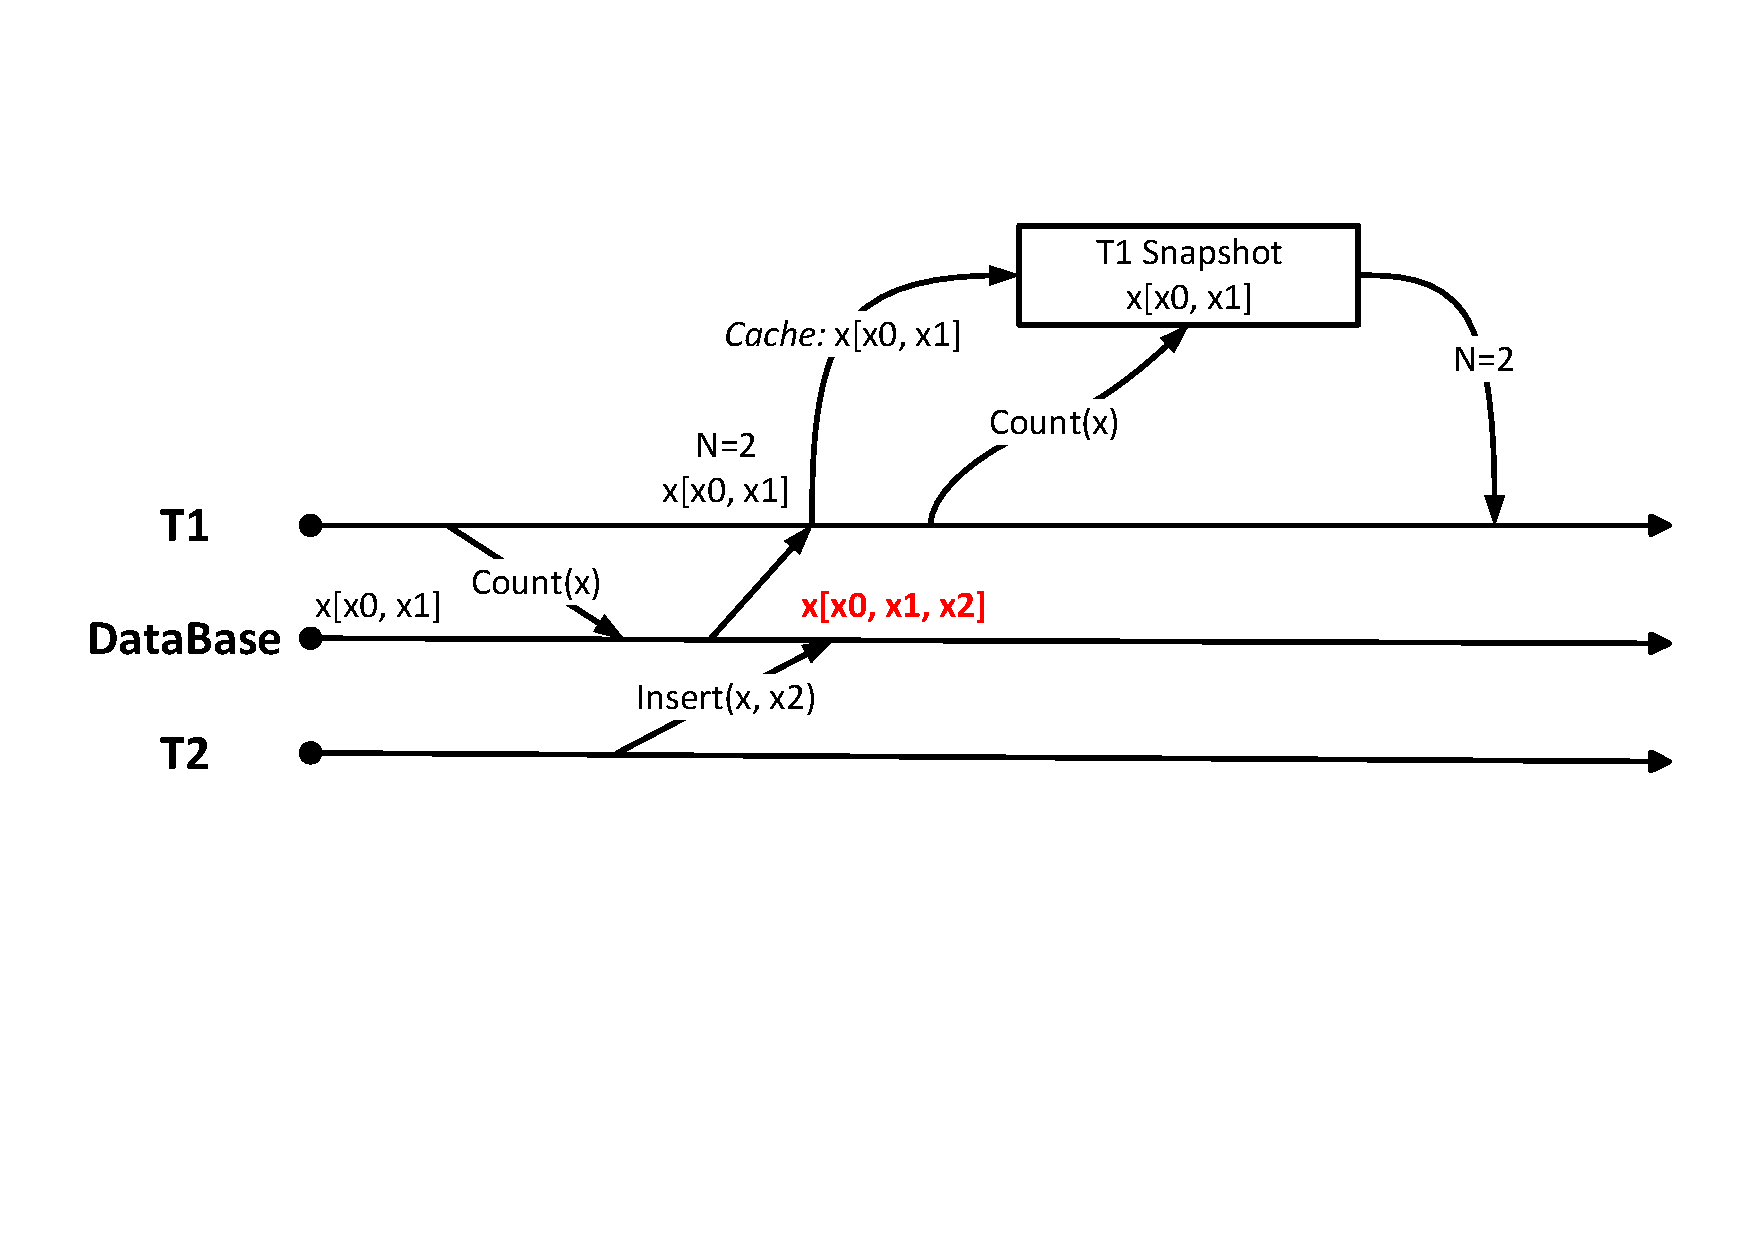
\includegraphics[width=\linewidth]{figs/snapphantom.pdf}
		\caption{Snapshot Isolation with Semantic Related Group Precludes Phantom Read}
		\label{fig:snapphantom}
	\end{figure}
	
\end{itemize} 
  %%%%%%%%%%%%%%%%%%%%%%%%%%%%%%%%%%%%%%%%%%%%%%%%%%%%%%%%%%%%%%%%%%%%%%%%%%%%%
  %
%%%%%                         ANOTHER SECTION
 %%%
  %
  
\section{ClusterJ and Lock Mode in MySQL Cluster}

\textit{ClusterJ}~\cite{mysqlclusterj} is a Java connector based on object-relational mapping persistence frameworks to access data in MySQL Cluster. Since it uses a JNI bridge to the NDB API for direct access to NDB Cluster, it doesn't depend on the MySQL Server to access data in MySQL Cluster, which means that ClusterJ can perform some operations much more quickly since it communicates to the data nodes directly. 

\noindent Therefore, with the mapping from java classes to database tables, we use ClusterJ to fetch and persist data in MySQL Cluster using primary key and unique key operations for single-table queries (not supporting multi-table operations though). If we recall the architecture of MySQL Cluster from Figure~\ref{fig:mysqlclusterarchitecture}, ClusterJ will be the Java Persistence API between Hop-HDFS and the \textit{Data Nodes} (ndbd) , without going through \textit{MySQL Servers} (mysqld).

\noindent Unlike \textit{two-phase locking} (2PL)~\cite{franklin1997concurrency}, there are three lock modes in MySQL Cluster:

\begin{enumerate}[noitemsep]
	\item \textbf{SHARED} (Read Lock, RL): Set a shared lock on rows
	\item \textbf{EXCLUSIVE} (Write Lock, WL): Set an exclusive lock on rows
	\item \textbf{READ\_COMMITTED} (Read Committed, RC): Set no locks but read the most recent committed values
\end{enumerate}

\noindent \textit{Shared} and \textit{Exclusive} locks have the same definition of those in Two-phase Locking. For \textit{Read\_Committed}, it is implemented for consistent nonlocking reads, which means that a fresh committed snapshot of data row is always presented to a query of database, regardless of whether Shared Lock or Exclusive Lock are taken on the current row or not. It is based on \textit{Multiversion Concurrency Control} described by Oracle~\cite{oraclemvcc} for read consistency from a single point in time (\textit{statement-level read consistency}). See Table~\ref{table:locktable} for the reference of the blocking effect.

\noindent We use \textit{Read\_Committed} for the \textit{read phase} in our algorithm.

\begin{table}[h]
	\centering
	\begin{tabular}{|c|c|c|c|}
		\hline
		\textbf{Lock Type} & \textbf{SHARED} & \textbf{EXCLUSIVE} & \textbf{READ\_COMMITTED} \\ \hline
		SHARED             & \checkmark               & Block              & \checkmark                        \\ \hline
		EXCLUSIVE          & Block           & Block              & \checkmark                        \\ \hline
		READ\_COMMITTED    & \checkmark               &            \checkmark        & \checkmark                        \\ \hline
	\end{tabular}
	\caption{Locks Blocking Table in MySQL Cluster}
	\label{table:locktable}
\end{table}
\section{Optimistic Concurrency Control}

Our algorithm is based on \textit{Optimistic Concurrency Control} (OCC) model to improve the overall read/write performance. Transactions are allowed to perform operations without blocking each other with optimistic methods. Concurrent transactions need to pass through a \textit{validation phase} to before committing, so that the serializability is not violated. Transactions will abort and restart if they fail in the \textit{validation phase}. OCC is the key approach to help remove the parent directory lock in Hop-HDFS so that transactions can operate under the same directory concurrently.

\noindent In \textit{read phase}, transactions use \textit{Read\_Committed Lock} to fetch semantic related group as snapshots and cache them in-memory for their own use.

\noindent In \textit{validation phase}, transactions will fetch the modified rows using \textit{Exclusive Lock} and fetch the semantic related rows using \textit{Shared Lock}. Then they compare the fetched values and the original copy of snapshot in the cache for their \textit{versions}. If they are all the same, go to \textit{update phase}. If not, abort current transaction, wait for a random milliseconds, and retry a new transaction from \textit{read phase}.

\noindent Note that using \textit{Shared Lock} to fetch semantic related rows can guarantee a consistent view in database until the transaction goes to the update phase, and also allows other Shared Locks taken on the same rows. 

\noindent In order to avoid multiple database round trips, we will do the fetching in batch processing provided by \textit{ClusterJ}.

\noindent \textit{Write skew} anomaly is precluded by the validation phase on the snapshot of semantic related group in OCC, because constraint violation on all related data rows will be checked before transaction committed. See Figure~\ref{fig:snapwriteskew} to see how optimistic concurrency control with snapshot isolation on semantic related group precludes \textit{Write Skew}.

\begin{figure}[h]
	\centering
	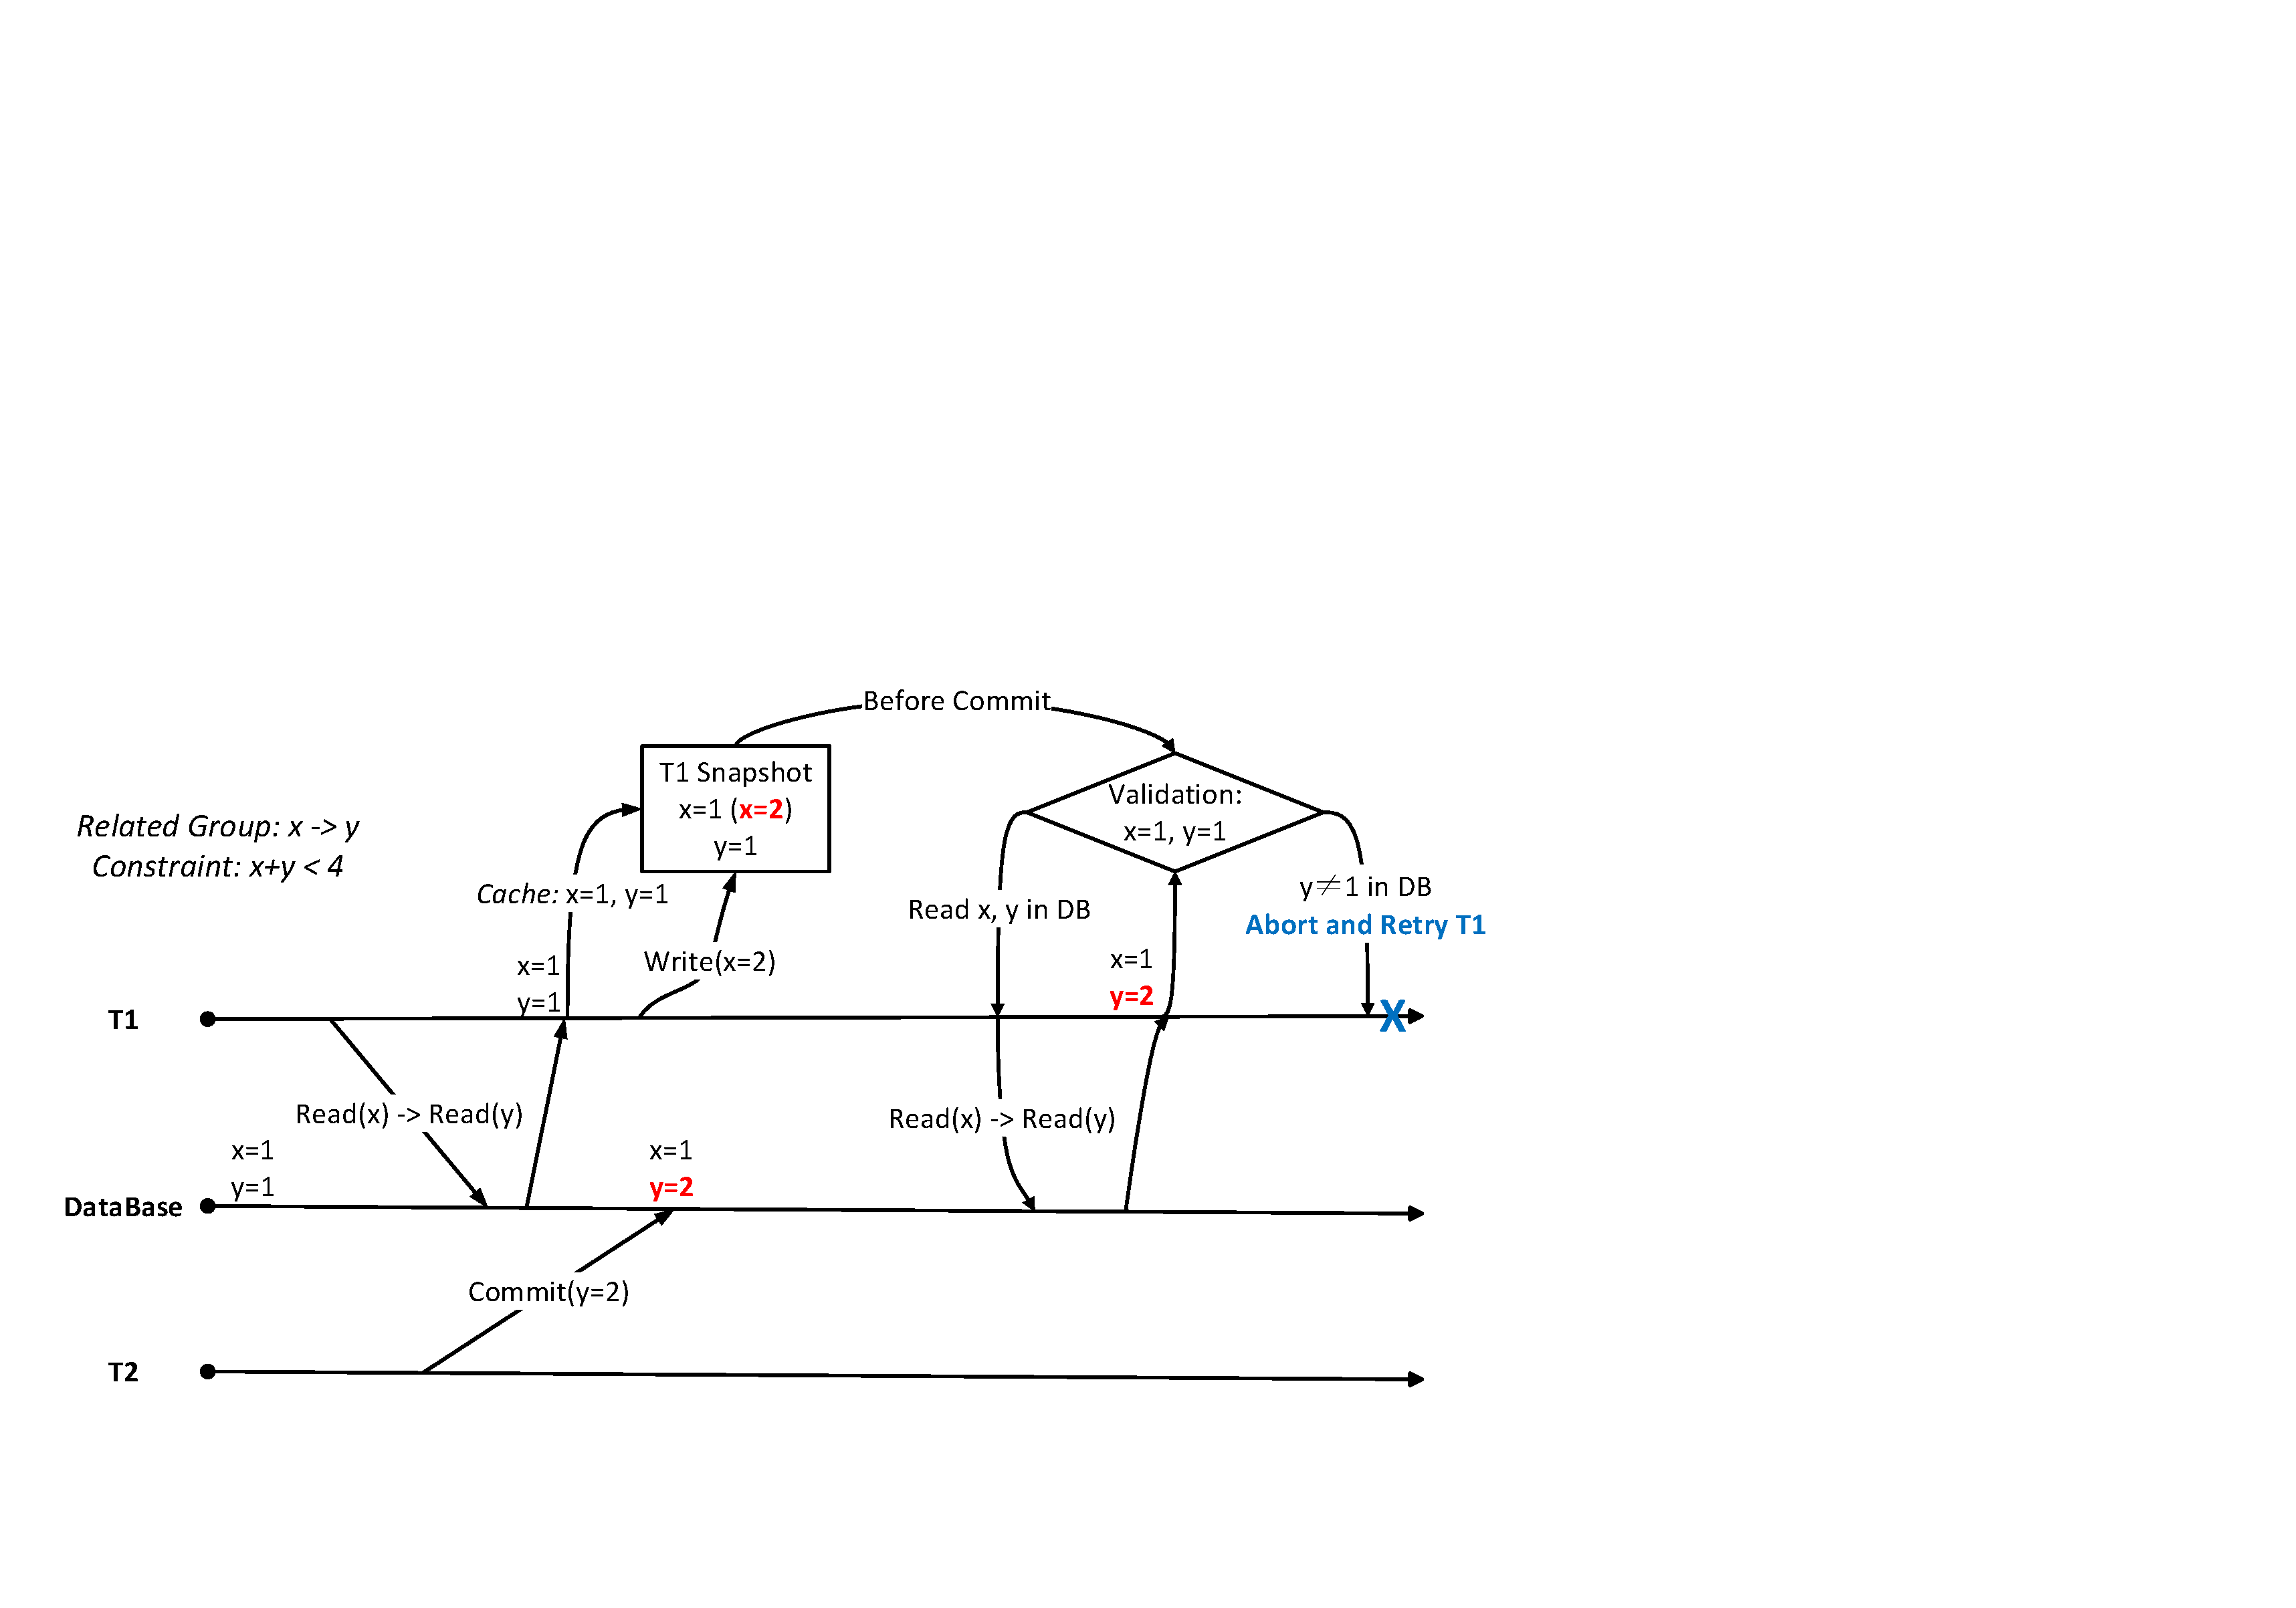
\includegraphics[width=\linewidth]{figs/snapwriteskew.pdf}
	\caption{Optimistic Concurrency Control with Snapshot Isolation on Semantic Related Group Precludes Write Skew}
	\label{fig:snapwriteskew}
\end{figure}

\noindent Therefore, we use optimistic concurrency control with snapshot isolation on semantic related group to improve the throughput while the strong consistency semantics in original HDFS is maintained.

\section{Total Order Update, Abort and Version Increase in Update Phase}
We have a total order update rule in update phase so that dead lock will not occur due to lock cycle. If multiple rows will be modified in a transaction during update phase, they will be sorted first by the \textit{id value}, then they will be updated in ascending order by their \textit{ids}. 

\noindent Since we can not take an Exclusive lock on the "new" row which not yet exists in the database beforehand, transactions may try to persist "new" with the same \textit{Primary Key} and one will be overwritten by the other. As we have defined the $<$name, parent\_id$>$ pair to be the \textit{Primary Key}, exception will be thrown when "duplicated" data is going to be persisted into the table by invoking \textit{makePersistent()} function in ClusterJ rather than \textit{savePersistent()} function.

\noindent The versions of the modified rows will be increased by 1 if they are successfully updated.
\section{Pseudocode of the Complete Algorithm}


  %%%%%%%%%%%%%%%%%%%%%%%%%%%%%%%%%%%%%%%%%%%%%%%%%%%%%%%%%%%%%%%%%%%%%%%%%%%%%
  %
%%%%%                 P A R T E   I V  --  Evaluation and Conclusion
 %%%
  %

\part{Evaluation and Conclusion}
\thispagestyle{empty}
%\vbox to\textheight{
%\vfil
%\chapter*{Omnis voluptas}
\thispagestyle{empty}

\newpage
\thispagestyle{empty}

  %%%%%%%%%%%%%%%%%%%%%%%%%%%%%%%%%%%%%%% -*- coding: utf-8; mode: latex -*- %%
  %
%%%%%                       CHAPTER
 %%%
  %

% $Id: 5100-omnis-voluptas.tex,v 1.1 2007/11/23 09:52:44 david Exp $
% $Log: 5100-omnis-voluptas.tex,v $
% Revision 1.1  2007/11/23 09:52:44  david
% *** empty log message ***
%
%

  %%%%%%%%%%%%%%%%%%%%%%%%%%%%%%%%%%%%%%%%%%%%%%%%%%%%%%%%%%%%%%%%%%%%%%%%%%%%%
  %
%%%%%                    HEAD MATTER
 %%%
  %

\chapter{Evaluation}
%\addcontentsline{lof}{chapter}{\thechapter\quad Nihil Molestiae}
%\addcontentsline{lot}{chapter}{\thechapter\quad Nihil Molestiae}
\label{ch:evaluation}

The solution \textit{Optimistic Concurrency Control with Snapshot Isolation on Semantic Related Group} (OCC) is built on top of the transactional framework~\cite{peiro2013maintaining} in the second version of Hop-HDFS (PCC). The goal of this chapter is to proof that our OCC model performs better than PCC. As a proof of concept, we implemented the OCC version for the operation \textit{mkdirs} and also give a detailed evaluation on it compared with the PCC version. For this purpose, we concern about the execution time (elapsed time) needed to finish all the concurrent tasks.

\section{Experimental Testbed}
\label{sec:testbed}

The MySQL Cluster consists of six data nodes connected by 1 Gigabit LAN. Each data node has an Intel Xeon X5660 CPU at 2.80GHz, and contributes 6 GB RAM (5 GB Data Memory + 1 GB Index Memory) separately. Therefore, the total available memory for the cluster is 36 GB. The number of data replicas is 2. The maximum concurrent transactions is 10000 for each data node, and the inactive timeout for each transaction is 5 seconds. 

\noindent To avoid any communication overhead caused by RPC connections and serialization, we run the NameNode and Clients on the same machine with Intel i7-4770T CPU at 2.50GHz and 16 GB RAM. This machine is connected with the MySQL Cluster data nodes by 100 Megabits LAN.

  %%%%%%%%%%%%%%%%%%%%%%%%%%%%%%%%%%%%%%%%%%%%%%%%%%%%%%%%%%%%%%%%%%%%%%%%%%%%%
  %
%%%%%                      SECOND SECTION
 %%%
  %

\section{Parent Directory Contention Assessment}
\label{sec:ww}

This experiment is the same as described in Section~\ref{sec:pdcassement}, but we expand it to include the results with OCC. See Figure~\ref{fig:hdfsPCCOCCparentDiragram} for the workload visual diagram. Here we have a full performance comparison here among HDFS, PCC and OCC.

\begin{figure}[ht]
	\centering
	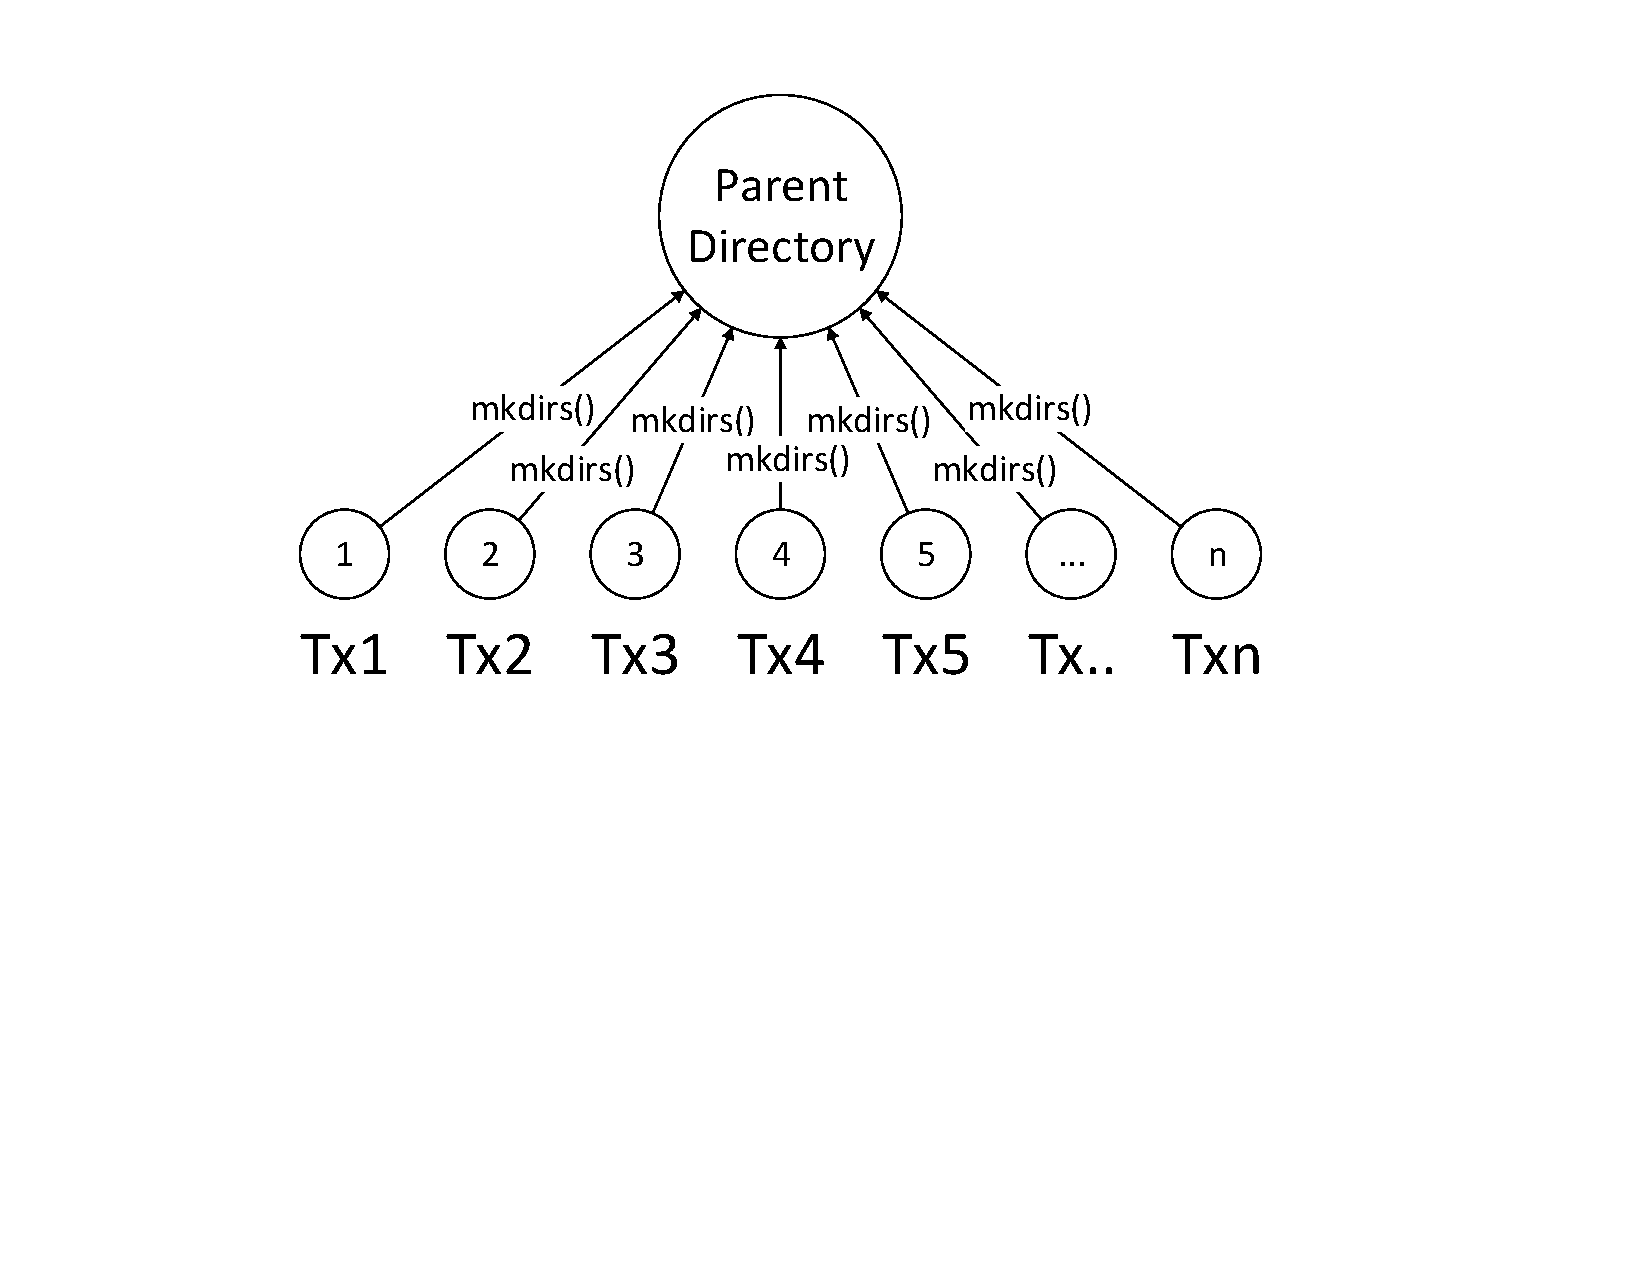
\includegraphics[scale=0.6]{figs/ww.pdf}
	\caption{Workload of Parent Directory Contention Assessment}
	\label{fig:hdfsPCCOCCparentDiragram}
\end{figure}

\noindent From Figure~\ref{fig:hdfsPCCOCCparent} and Table~\ref{fig:hdfsPCCOCCparent}, we can see that OCC significantly outperforms PCC by almost 70 \% on this concurrent write-write parent directory contention workload. Under heavy workload, the execution time is just 1.3 times of HDFS. Remember that this is just a single NameNode performance test. We believe that OCC can much better outperform HDFS in our multiple NameNodes architecture.

\begin{figure}[ht]
	\centering
	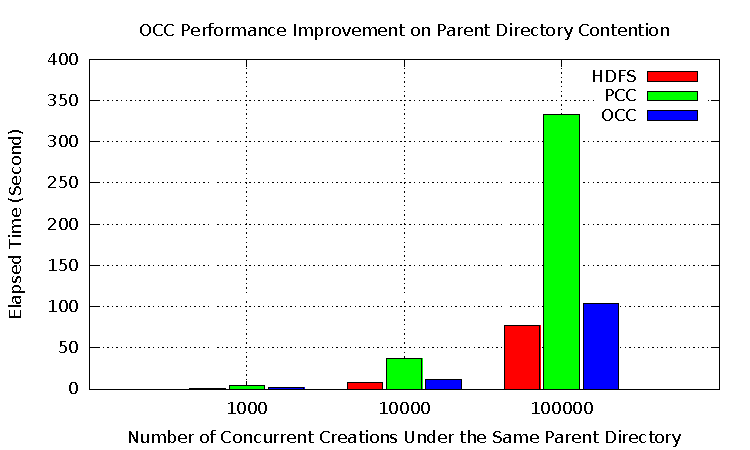
\includegraphics[width=\linewidth]{figs/hdfs_pcc_occ_parent.pdf}
	\caption{OCC Performance Improvement on Parent Directory Contention}
	\label{fig:hdfsPCCOCCparent}
\end{figure}

\begin{table}[ht]
	\centering
	\begin{tabular}{|c|c|c|c|}
		\hline
		\textbf{Num. of Concurrent Creation}                                                 & \textbf{1000}   & \textbf{10000}  & \textbf{100000} \\ \hline
		HDFS                                                                                 & 0.82s           & 7.83s           & 77.13s          \\ \hline
		PCC                                                                                  & 4.35s           & 36.74s          & 332.36s         \\ \hline
		OCC                                                                                  & 1.36s           & 12.01s          & 103.23s         \\ \hline
		PCC / HDFS                                                                           & 530.5\%         & 469.2\%         & 430.9\%         \\ \hline
		OCC / HDFS                                                                           & 165.9\%         & 153.4\%         & 133.8\%         \\ \hline
		\textbf{\begin{tabular}[c]{@{}c@{}}OCC Improvement: \\ (PCC-OCC) / PCC\end{tabular}} & \textbf{68.7\%} & \textbf{67.3\%} & \textbf{68.9\%} \\ \hline
	\end{tabular}
	\caption{OCC Performance Improvement on Parent Directory Contention}
	\label{table:hdfsPCCOCCparent}
\end{table}

\section{Read-Write Mixed Workload Assessment}

In this experiment, we did a test for a read-write mixed workload assessment while the parent directory is still the contention point for PCC. So we assume that OCC will still outperform PCC in this kind of workload. 

\noindent Similar to the experiment in Section~\ref{sec:ww}, we have 1000, 10000 and 100000 concurrent clients' operations running under the same parent directory. But in each task, half of them will do the metadata read operation \textit{getFileStatus()}, while the other half will do the write operation \textit{mkdirs()}. See Figure~\ref{fig:rwWorkload} for a visual reference.

\begin{figure}[ht]
	\centering
	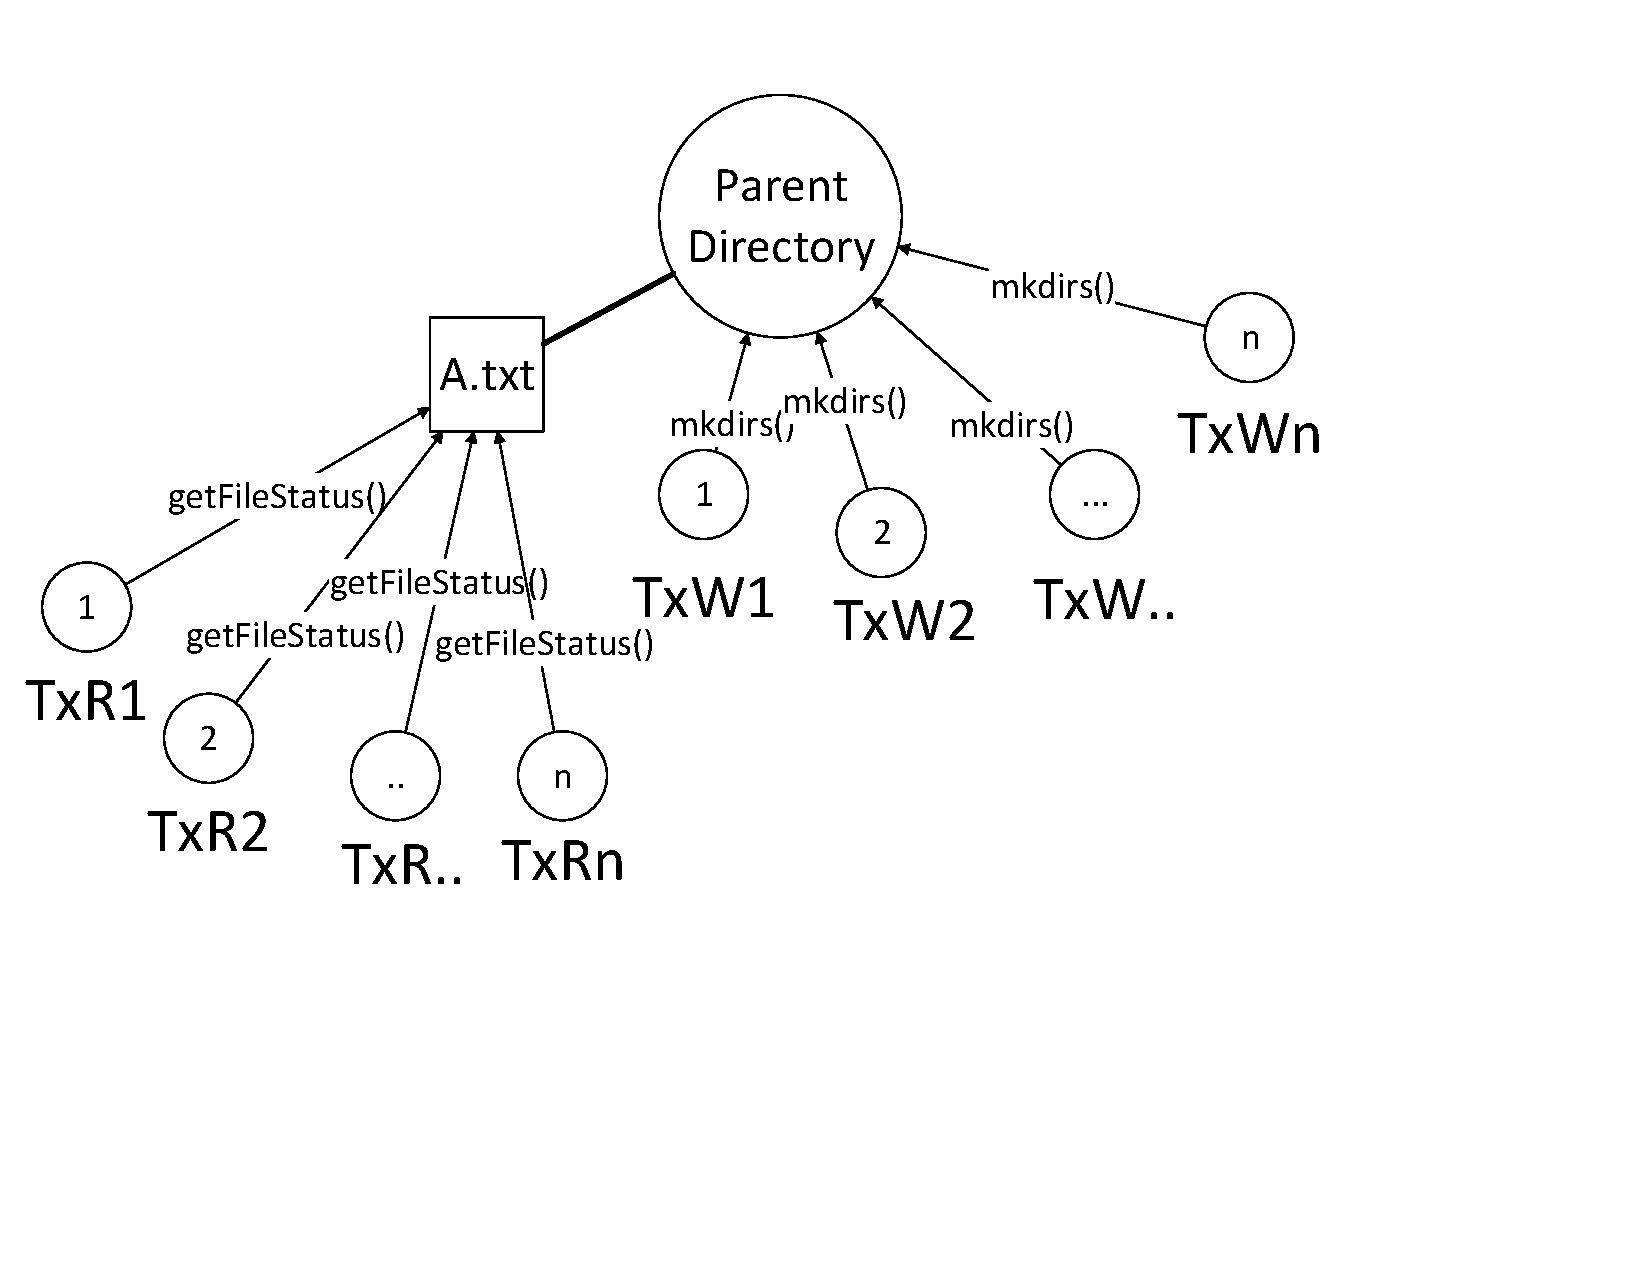
\includegraphics[scale=0.6]{figs/rw.pdf}
	\caption{Read-Write Mixed Workload}
	\label{fig:rwWorkload}
\end{figure}

\noindent From Figure~\ref{fig:rwWorkload} and Table~\ref{fig:rw}, we can see that OCC still significantly outperforms PCC by 65 \% on this concurrent read-write mixed workload. 

\begin{figure}[ht]
	\centering
	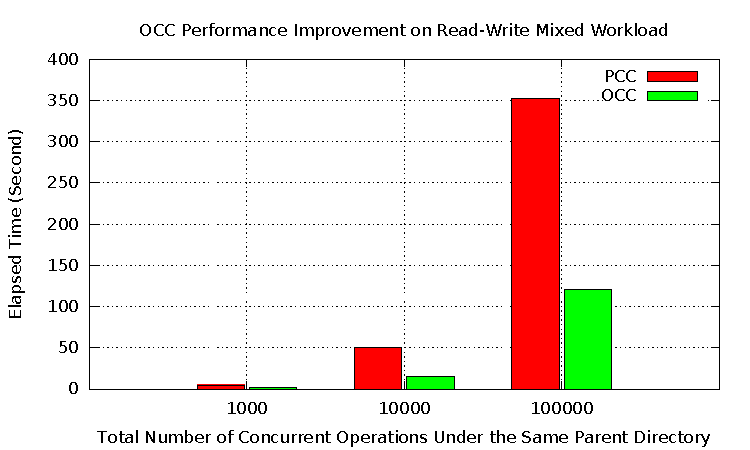
\includegraphics[width=\linewidth]{figs/pcc_occ_rw.pdf}
	\caption{OCC Performance Improvement on Read-Write Mixed Workload}
	\label{fig:rw}
\end{figure}

\begin{table}[ht]
	\centering
	\begin{tabular}{|c|c|c|c|}
		\hline
		\textbf{Num. of Concurrent Creation}                                                 & \textbf{1000}   & \textbf{10000}  & \textbf{100000} \\ \hline
		PCC                                                                                  & 4.92s           & 50.69s          & 352.25s         \\ \hline
		OCC                                                                                  & 1.78s           & 15.31s          & 120.64s         \\ \hline
		\textbf{\begin{tabular}[c]{@{}c@{}}OCC Improvement: \\ (PCC-OCC) / PCC\end{tabular}} & \textbf{63.8\%} & \textbf{69.8\%} & \textbf{65.8\%} \\ \hline
	\end{tabular}
	\caption{OCC Performance Improvement on Read-Write Mixed Workload}
	\label{table:rw}
\end{table}

\section{The Size of Semantic Related Group}

In the read phase and validation phase, we need to fetch the semantic related group. The more levels of directories involved, the more related data rows needs to be fetch. The depth of the path equals to the size of the semantic related group. 
\noindent But since the namespace is a tree structure, the depth of the namespace won't be too much due to the logarithmic order. Also, HDFS limits the maximum number of levels to be 1000, and maximum number of characters for the full path name to be 3000~\footnote{If we assume that 10 characters for one directory name, the maximum level will be 300.}. 

\noindent In addition, batch reading is also used to minimize the network round-trips so that multiple data can fetched in one round-trip. Therefore, the size of semantic related group will not be a limitation in practice. 

\noindent Here we did a test to see how performance affected by different size of semantic related group. Similar to the experiment in Section~\ref{sec:ww}, we have 100 concurrent operations (\textit{mkdirs()}) running under the same parent directory. See Figure~\ref{fig:srg} for the linear relationship between the size and the elapsed time.

\begin{figure}[ht]
	\centering
	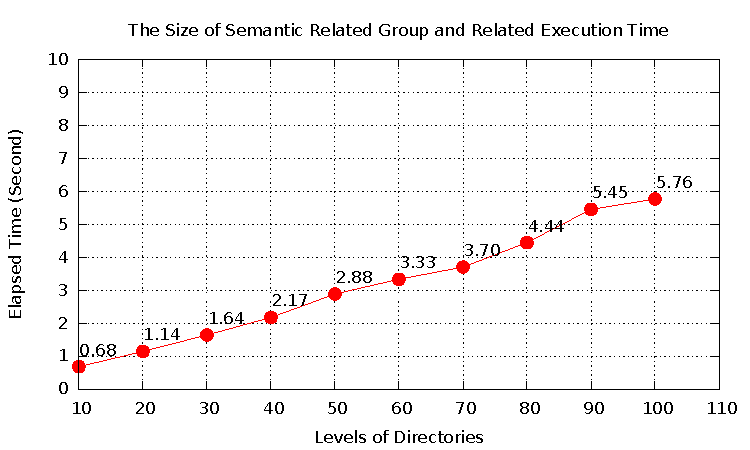
\includegraphics[width=\linewidth]{figs/srgSize.pdf}
	\caption{The Size of Semantic Related Group and Related Execution Time}
	\label{fig:srg}
\end{figure}

\section{OCC Performance with Different Size of Conflicts}

When OCC conflicts happen, transactions will abort, wait for random milliseconds and retry. Eventually one transaction will success, and others will get updated values after retry and return RPC callbacks.

\noindent Here we have 10000 concurrent operations running under the same parent directory. Each operation creates only one sub-directory. Some of them will success and some others will fail due to conflicts. These operations will try to create same sub-directories in different numbers from 1 (all conflicts), to 10000 (no conflicts). Therefore, we have different size of conflicts.

\begin{figure}[ht]
	\centering
	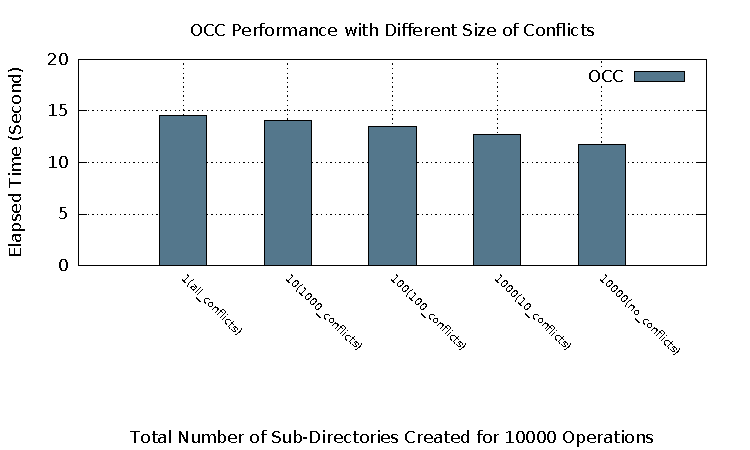
\includegraphics[width=\linewidth]{figs/conflict.pdf}
	\caption{OCC Performance with Different Size of Conflicts}
	\label{fig:conflict}
\end{figure}

\begin{table}[ht]
	\centering
\begin{tabular}{|c|c|}
	\hline
	\textbf{Total Num. of Sub-DirectoriesCreated for 10000 Operations} & \textbf{Elapsed Time (Second)} \\ \hline
	1 (all conflicts)                                                  & 14.53                          \\ \hline
	10 (1000 conflicts)                                                & 14.11                          \\ \hline
	100 (100 conflicts)                                                & 13.51                          \\ \hline
	1000 (10 conflicts)                                                & 12.72                          \\ \hline
	10000 (no conflicts)                                               & 11.75                          \\ \hline
\end{tabular}
	\caption{OCC Performance with Different Size of Conflicts}
	\label{table:conflicts}
\end{table}

\noindent From Figure~\ref{fig:rwWorkload} and Table~\ref{fig:rw}, we can calculate that the maximum performance degradation is 19.1\% when all operations conflict:
\begin{center}
	$(14.53-11.75) \div 14.53 = 19.1\%$
\end{center}

\section{Correctness Assessment}

The correctness of our OCC implementation for \textit{mkdirs()}~\footnote{other operations are PCC} has been validated by 300+ Apache HDFS 2.0.4 Alpha unit tests passing. The full passing tests list can be found in Appendix~\ref{ch:Testing}.                 
  %%%%%%%%%%%%%%%%%%%%%%%%%%%%%%%%%%%%%%% -*- coding: utf-8; mode: latex -*- %%
  %
%%%%%                       CHAPTER
 %%%
  %

% $Id: 7200-magna-aliqua.tex,v 1.1 2007/11/23 09:52:46 david Exp $
% $Log: 7200-magna-aliqua.tex,v $
% Revision 1.1  2007/11/23 09:52:46  david
% *** empty log message ***
%
%

  %%%%%%%%%%%%%%%%%%%%%%%%%%%%%%%%%%%%%%%%%%%%%%%%%%%%%%%%%%%%%%%%%%%%%%%%%%%%%
  %
%%%%%                    HEAD MATTER
 %%%
  %

\chapter{Conclusion}
%\addcontentsline{lof}{chapter}{\thechapter\quad Nihil Molestiae}
%\addcontentsline{lot}{chapter}{\thechapter\quad Nihil Molestiae}
\label{ch:Conclusion}

%\begin{quotation}
%  {\small\it Neque porro quisquam est qui dolorem ipsum quia dolor sit amet, consectetur, adipisci velit...}
%
%{\small\it -- Cerico}
%\end{quotation}



  %%%%%%%%%%%%%%%%%%%%%%%%%%%%%%%%%%%%%%%%%%%%%%%%%%%%%%%%%%%%%%%%%%%%%%%%%%%%%
  %
%%%%%                        FIRST SECTION
 %%%
  %

\section{A}

AAA

  %%%%%%%%%%%%%%%%%%%%%%%%%%%%%%%%%%%%%%%%%%%%%%%%%%%%%%%%%%%%%%%%%%%%%%%%%%%%%
  %
%%%%%                      SECOND SECTION
 %%%
  %

\section{B}

BBB

  %%%%%%%%%%%%%%%%%%%%%%%%%%%%%%%%%%%%%%%%%%%%%%%%%%%%%%%%%%%%%%%%%%%%%%%%%%%%%
  %
%%%%%                         ANOTHER SECTION
 %%%
  %
\section{C}

CCC

  %%%%%%%%%%%%%%%%%%%%%%%%%%%%%%%%%%%%%%%%%%%%%%%%%%%%%%%%%%%%%%%%%%%%%%%%%%%%%
  %
%%%%%                          LAST SECTION
 %%%
  %
            

  %%%%%%%%%%%%%%%%%%%%%%%%%%%%%%%%%%%%%%%%%%%%%%%%%%%%%%%%%%%%%%%%%%%%%%%%%%%%%
  %
%%%%%                        SPECIAL
 %%%
  %
%\bibliographystyle{authordate3}             % Bibliography
%\bibliographystyle{apacitex}
\bibliographystyle{chicago}
\bibliography{reference}
%---------------------------------------------------------------------------
%\begin{singlespace}
%\printindex[autx]\cleardoublepage            % Author index (apacitex)
%\end{singlespace}

  %%%%%%%%%%%%%%%%%%%%%%%%%%%%%%%%%%%%%%%%%%%%%%%%%%%%%%%%%%%%%%%%%%%%%%%%%%%%%
  %
%%%%%                         APPENDIX
 %%%
  %

\part{Appendices}
\appendix
%
  %%%%%%%%%%%%%%%%%%%%%%%%%%%%%%%%%%%%%%% -*- coding: utf-8; mode: latex -*- %%
  %
%%%%%                     APPENDIX
 %%%
  %

% $Id: 9100-commodo-consequat.tex,v 1.1 2007/11/23 09:52:47 david Exp $
% $Log: 9100-commodo-consequat.tex,v $
% Revision 1.1  2007/11/23 09:52:47  david
% *** empty log message ***
%
%

  %%%%%%%%%%%%%%%%%%%%%%%%%%%%%%%%%%%%%%%%%%%%%%%%%%%%%%%%%%%%%%%%%%%%%%%%%%%%%
  %
%%%%%                           HEAD MATTER
 %%%
  %

\chapter{Apache HDFS Unit Tests Passing List}
%%\addcontentsline{lof}{chapter}{\thechapter\quad Commodo Consequat}
%%\addcontentsline{lot}{chapter}{\thechapter\quad Commodo Consequat}
\label{ch:Testing}
%
\begin{figure}[ht]
  \centering
  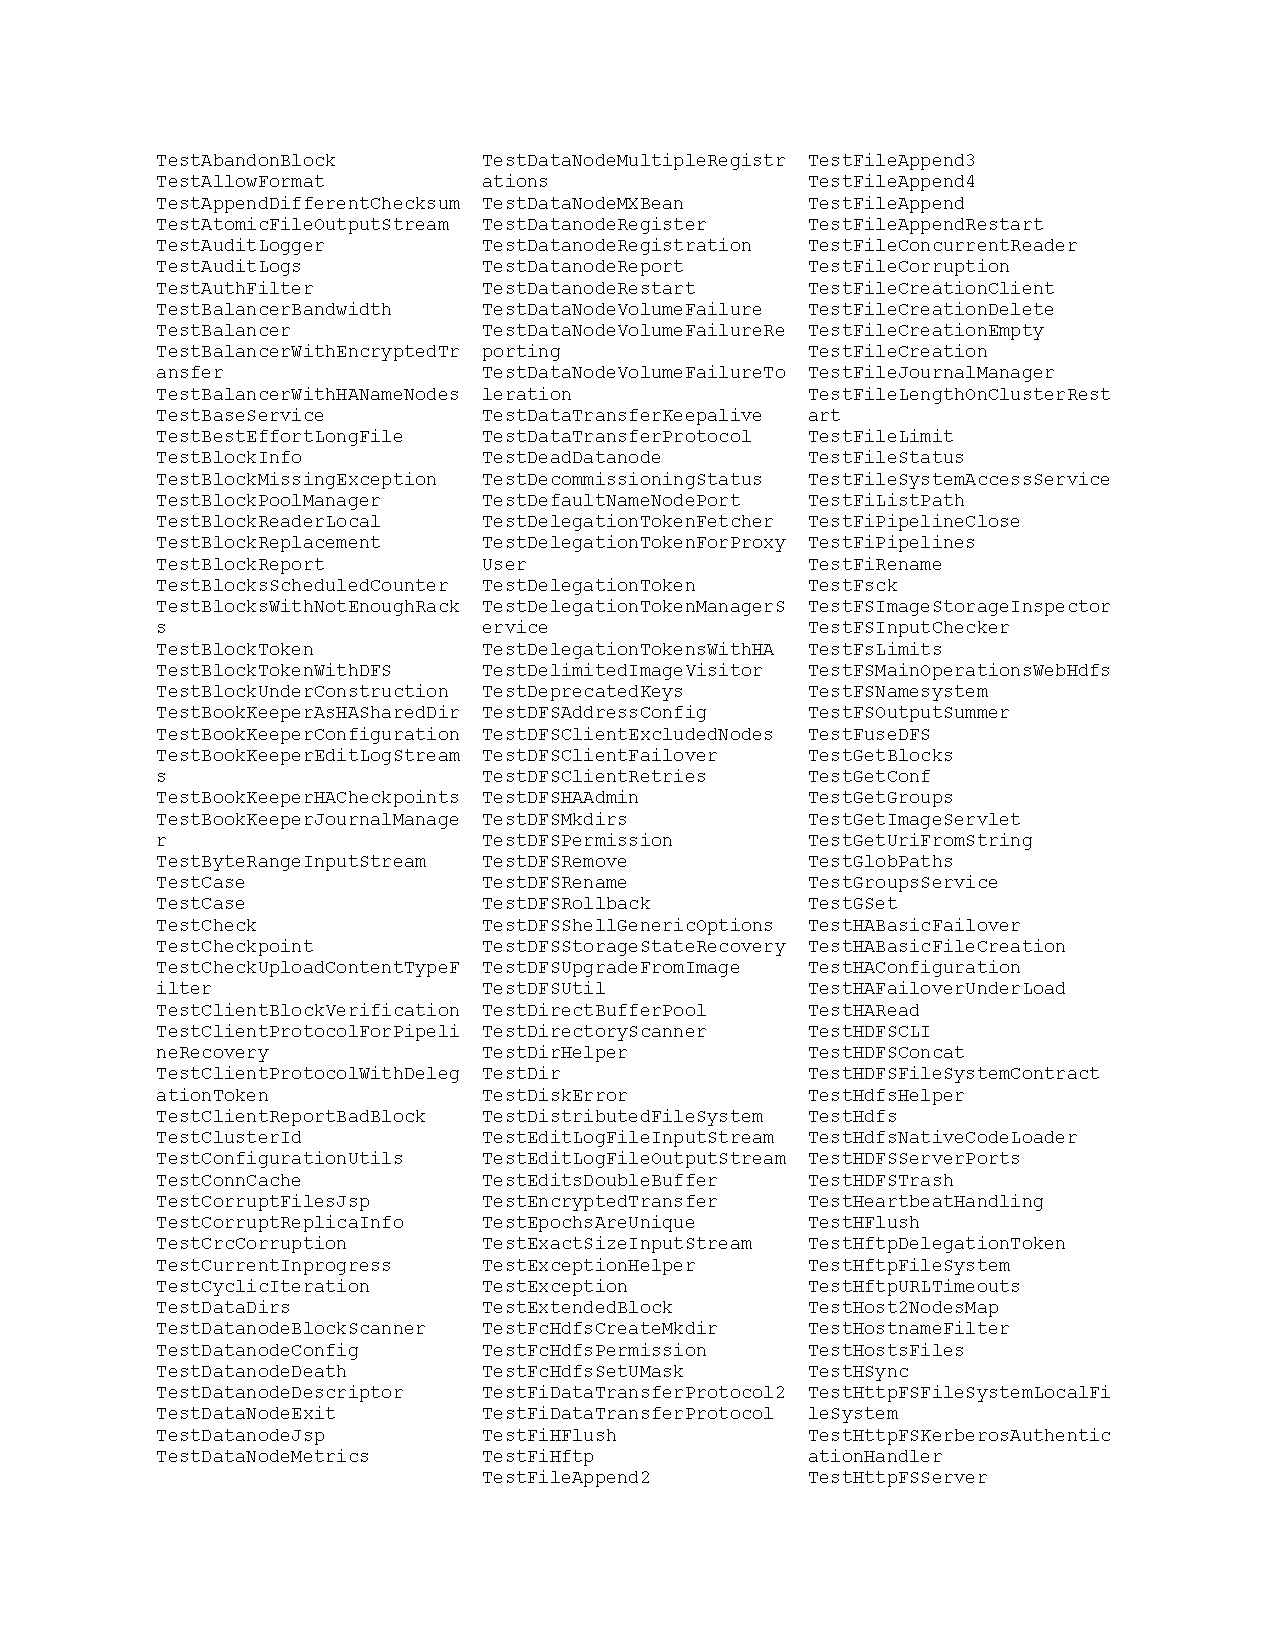
\includegraphics[width=\linewidth]{figs/unitTest1.pdf}
  \caption{Apache HDFS 2.0.4 Alpha Unit Tests Passing List 1}
  \label{fig:unit1}
\end{figure}
\begin{figure}[ht]
	\centering
	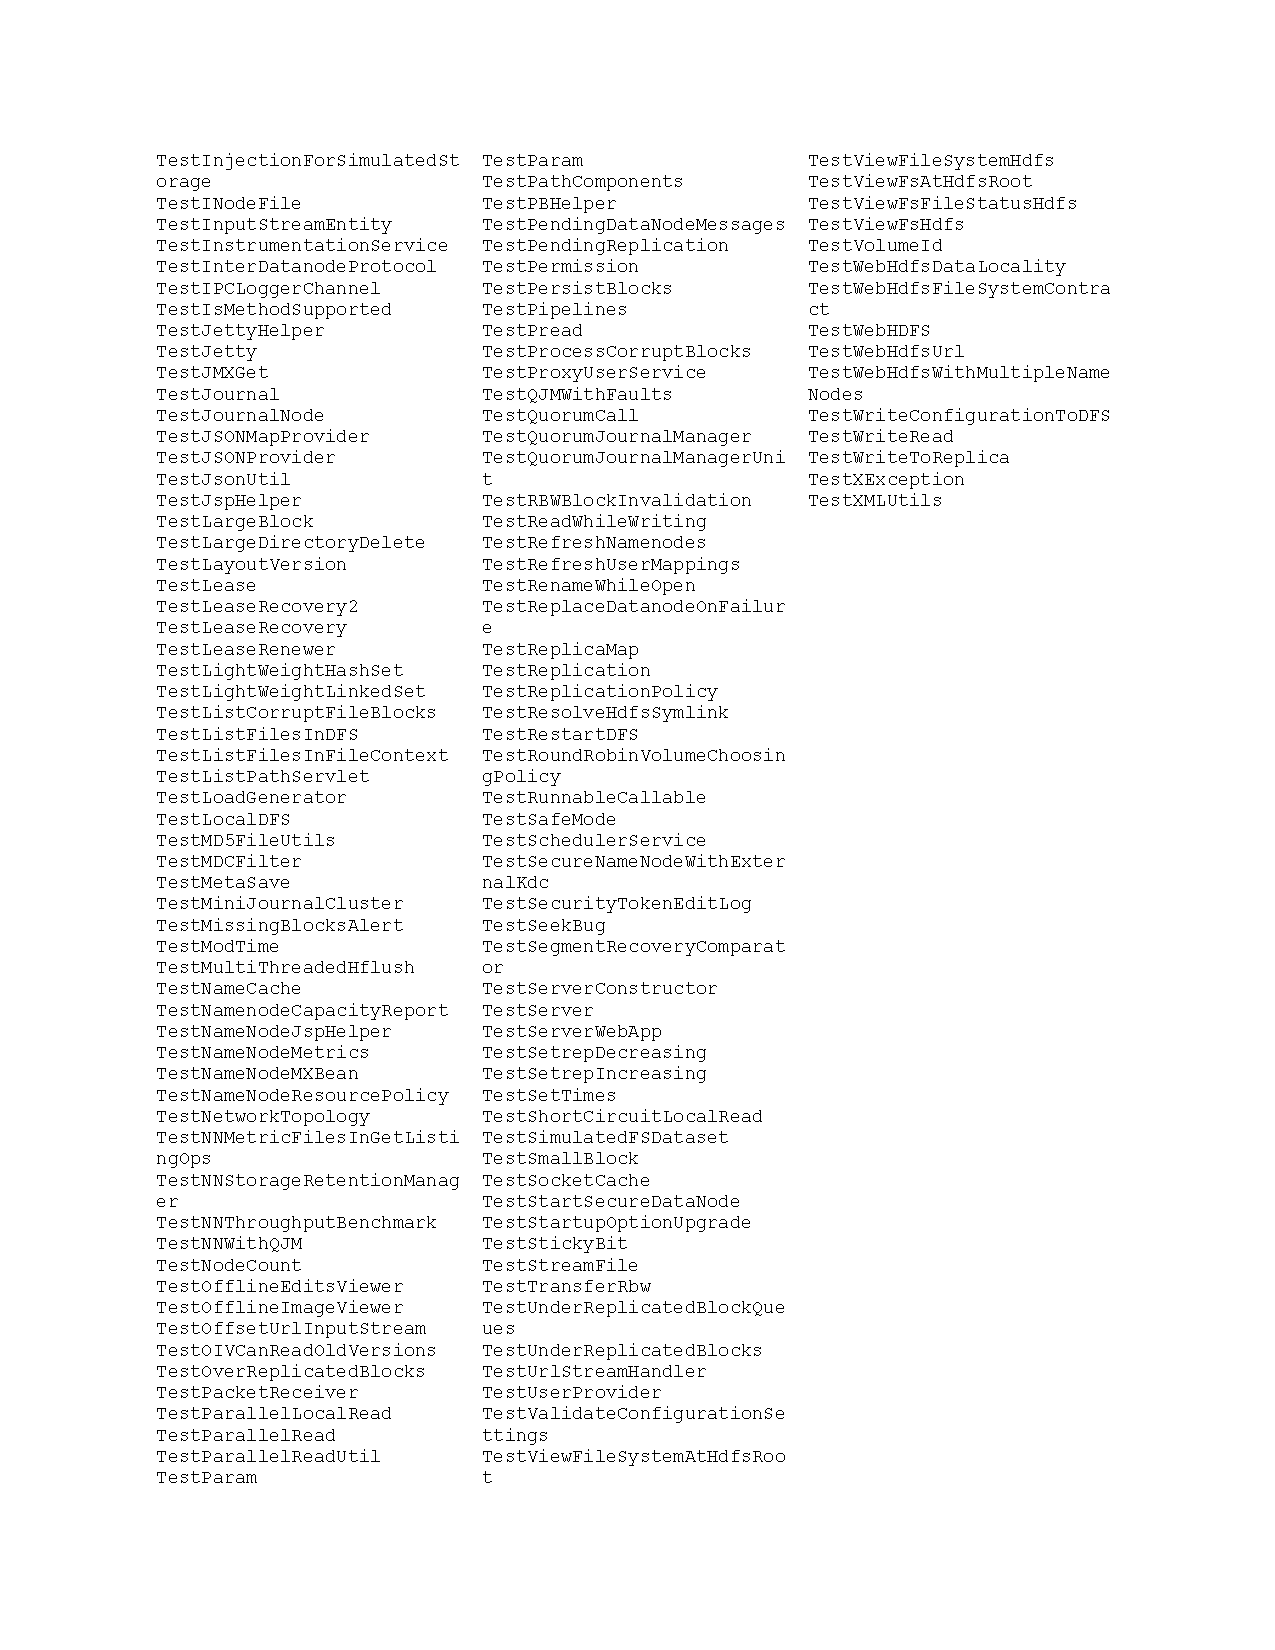
\includegraphics[width=\linewidth]{figs/unitTest2.pdf}
	\caption{Apache HDFS 2.0.4 Alpha Unit Tests Passing List 2}
	\label{fig:unit2}
\end{figure}

         % commodo consequat

%\begin{singlespace}
%\printnomenclature\cleardoublepage               % Glossary
%\end{singlespace}


  %%%%%%%%%%%%%%%%%%%%%%%%%%%%%%%%%%%%%%%%%%%%%%%%%%%%%%%%%%%%%%%%%%%%%%%%%%%%%
  %
%%%%%                         SPECIAL
 %%%
  %
\begin{singlespace}

\def\indexname{Index}             % Index
\printindex\cleardoublepage

\end{singlespace}

\end{document}

  %
 %%%
%%%%%                          THE END
  %
  %%%%%%%%%%%%%%%%%%%%%%%%%%%%%%%%%%%%%%%%%%%%%%%%%%%%%%%%%%%%%%%%%%%%%%%%%%%%%
